%%%%%%%%%%%%%%%%%%%%%%%%%%%%%%%%%%%%%%%%%%%%%%%%%%%%%%%
% Copied from previous \section{Neural Network Training}
In the VBF-enriched \TwoJet category, a DNN-based binary classifier is used as a final discriminant.
This section describes how this DNN, referred to as \emph{VBF DNN} in the following, is developed using supervised learning with simulated $pp$ collision events.
The relevant ML concepts are introduced in \cref{chap:ml}.
The DNN is developed using industry-standard open-source ML libraries, integrated in a self-developed software framework that has been continuously developed during the course of the author's PhD to manage the full ML cycle efficiently. The entire software suite used is summarized in \cref{app:software-suite}.

\subsection{Methodology and historical developments}
Implementing a neural network model into a physics analysis is a multi-stage procedure. 

\paragraph{Stage 1}
The first step is to prepare the training data.
The simulated samples that are listed in \cref{subsec:simulated-event-samples} are therefore transformed in a way, so they can be easily used with state-of-the-art ML software. Details on the training data are given in \cref{subsec:training-data}

\paragraph{Stage 2}
The second stage is the main part of the development and involves the training, validation, and optimization of the DNN. The details of this iterative workflow are presented in \cref{subsec:hyper-parameters}.

\paragraph{Stage 3}
The third step is to deploy the neural network in the \HWW\ analysis and produce final measurement results. This provides the ultimate performance metric of the trained DNN model, and reveals the weak-spots of the analysis and the developed model. The latter information can be used to adapt the training procedure in stage two and further improve the DNN model. 
How this was done for the VBF DNN is described in \cref{subsec:sample-fraction-optimization}.

\paragraph{Final model selection}
The final DNN model is selected when no further improvements can be made by repeating stage two and three. It should be noted that the tasks of stage three are very time-consuming and computing-expensive, which limits the number of cycles that can realistically be carried out.
It should also be noted that the training procedure has been modified several times during the course of the author's PhD, due to both improvements in the self-developed software and historical developments of the \HWW\ analysis (for example changes in MC simulated samples). If not mentioned otherwise, the results and procedures presented correspond to the final VBF DNN. 
% that improvements of the self-developed software, together with historical developments of the entire \HWW\ analysis, lead to several modifications of the training setup over time. 

% During the course of the author's doctoral studies, some approaches have evolved, which means that certain parts of the training procedure have been optimized based on earlier versions of the training setup than the version used for the final DNN. 
% The following outlines roughly the different stages of the training, to motivate the procedures and decisions that were taken that resulted in the development of the final DNN used in this analysis. 
% The hyperparameters and procedure used for the final DNN are summarized in \cref{tab:hyper-parameters}.

%%%%%%%%%%%%%
% DISTINGUISH??: Physics based optimization, DNN based, empirical optimization

% - Historical developments, features freezes, limitations of computing resources/turnaround time
% The following therefore is an attempt to only a rough outline of the different stages of the training, which, due to both historical developments and the empirical nature of ML, should not be taken at face value but rather viewed as an attempt to roughly describe the approaches and procedures that have led to the development of the final DNN. 


\subsection{Training data}
\label{subsec:training-data}
- At b-veto cut stage
- The data is labelled to distinguish VBF signal events, $t_n = 1$, from all other types of events, $t_n = 0$, where $t_n$ is the \emph{target} value for event $n$.
% The ground-truth labels (called \emph{targets}), $t_n$, are set to $t_n = 1$, for VBF signal events, and $t_n = 0$ otherwise, to prepare the data for the supervised learning algorithm.
- normalized to their theoretical cross-section predictions.
- List of training events per process


\subsection{Hyperparameters and performance metrics}
\label{subsec:hyper-parameters}
% The optimization problem is multi-dimensional, which means that, for example, optimising a parameter $B$ after optimising parameter $A$ may result in the value of parameter $A$ no longer being optimal.
The optimization and choice of hyperparameters is a vastly empirical procedure.
The complete set of hyperparameters chosen for the final VBF DNN is summarized in \cref{tab:DNN-info}. 

The model architecture used is a feedforward DNN with one output layer that uses a logistic sigmoid as activation function. All other nodes use the ReLU function as activation functions. 

The batchsize is chosen to be 512.

The binary cross-entropy loss is used as loss function during the training.
Adagrad optimizer with additional learning rate decay.
\Cref{fig:monitoring} shows how the loss and binary accuracy is monitored during the training. The binary accuracy is defined by counting a VBF signal event (non-VBF-signal event) as correctly classified if the DNN output value is larger (smaller) 0.5.

- Dropout is used for regularisation by randomly disabling 20\% of weights between each layer for each batch of data. 

%%%%%%%%%%%%%%%%%%%%%%%%%%%%%%%%%%%
% Performance metric explanation
The discovery significance (see \cref{chap:statistics}) of the VBF signal process over the non-VBF-signal processes is used as a performance metric to optimize the hyperparameters and select the final model.

The significance is computed based on a histogram with several bins of the output of the neural network. It corresponds to the square root of the sum of the squared significances calculated in each of the bins according to \cref{eq:discovery-significance}. 
This metric is driven by the bins with the highest signal purity and is therefore sensitive to the choice of binning. In order to mitigate the impact of the binning choice on the performance metric, a variable binning is used. This allows for a fair comparison between different neural network models, in particular if they exhibit different shapes. The binning of the histograms is determined with the same procedure as the binning of the final discriminant in the statistical analysis. 
\cref{fig:dnn-val-set}

The $k$-fold cross validation method is used to avoid any bias and the final model is selected based on the significance corresponding to the validation set. 
The test set is used as a final validation to ensure generalisation. 

Model choice: Choose model with highest significance in validation set!
Model validation: Validate model comparing against test set!

\captionsetup[subfloat]{captionskip=7pt} % space between subfloat caption and image
% Plots made with SFUsMLKit on cedar with:
% ./plot.py -c configs/HWW/winningSubmission.cfg --trainingFolderName dropout-02-5-fold-aggressive-lr-schedule-2-fine-scan-ewww-scan-etafix/210805_9_0.12_8226149877761426764
\begin{figure}[t]
    \subfloat[] {
        \newImageResizeCustom{0.47}{figures/hww/dnn/CutVBF_SR_reTrained_default_optBinning.pdf}
    }
    \subfloat[] {
        \newImageResizeCustom{0.47}{figures/hww/dnn/CutVBF_SR_reTrained_default_optBinning_zoom.pdf}
    }
    \caption{DNN output distribution corresponding to the validation set of the training data for (a) the full range of DNN output values and (b) the region with high VBF signal purity. The binning is chosen as explained in the text.}
    \label{fig:dnn-val-set}
\end{figure}



% \paragraph{Iteration 1 - establish robust training}
% \begin{itemize}
%     \item reLU activation, sigmoid as output activation, cross-entropy loss
%     \item batchsize: chosen to be 512
%     \item learning rate, optimizer: adagrad (adaptive learning rate! (no need to overoptimize it))
%     \item prelim regularisation
%     \item prelim. architecture: layers = 128, 64, 32, 24, 16, 8
% \end{itemize}
% \paragraph{Iteration 2 - find set of features}
% \begin{itemize}
%     \item optimize set of input features
%     \item Optimize architectures
%     \item Adjust dropout (repeat)
% \end{itemize}
% \paragraph{Iteration 3 - final optimization}
% \begin{itemize}
%     \item Use and optimize k-fold method (5-fold is enough)
%     \item optimize physics weights while scanning for optimal learning rate
% \end{itemize}
% The physics related parameters are the set of input features (observables), and the weights corresponding to different processes in training dataset. 
% % ML related
% % - network architecture
% % - learning rate (batch size)
% % - optimizer
% % - regularization technique
% % - choice of k-fold method
% The training procedure in stage 1 and stage 2 was following a 70/10/20 split of training and test sample. This means, 70\% of the training data was used directly for the training, 10\% for validation during the training, and 20\% to test the final model. The simple significance as shown in \cref{eq:simple-sign} using statistical uncertainties only is used as a performance metric.
% In stage 3, the k-fold cross-validation is used, as explained in \cref{chap:ml}, and an additional performance metric is considered that is based on the knowledge about systematic uncertainties established in previous iterations of the analysis. The systematic uncertainties of the background processes are used in \cref{eq:simple-sign}. The difference between the significances can be seen in \cref{fig:significance-final-optimization}.




\begin{table}[ht]
    \begin{center}
    
\begin{tabular}{l l}
    \toprule
    Parameter/Characteristic & Value \\
    \midrule
    Input layers & 15 \\ 
    \multirow{2}{*}{Input variables}  & \mjj, \dyjj, \lepetacent, \mlonejone, \mlonejtwo, \mltwojone, \mltwojtwo, \\
    & \pTjone, \pTjtwo, \pTjthree, \dphill, \mll, \mT, \pttot, \METSig\\ 
    Hidden layers & {256, 128, 64, 32, 24, 16, 8} \\
    Activation & ReLU \\ 
    Output layers & 1 \\
    Output activation & sigmoid \\ 
    Loss function & cross-entropy \\ 
    Learning rate & 9 \\
    Batchsize & 512 \\ 
    Optimizer & AdaGrad \\
    Dropout &  20\% \\ 
    Epochs & 40 \\
    Training weights & optimized \\ 
    Training sets/folds & 5 folds (train/val/test) \\
    \bottomrule
\end{tabular}

    \end{center}
    \caption{Hyperparameters and training procedure used for the development of the final VBF DNN.
    }
    \label{tab:DNN-info}
    % Nominal values, statistical uncertainties and EWSUBTR uncertainties produced on tag kon_improveZjetsFFStats_v2
\end{table}

\begin{figure}[t]
    \subfloat[] {
        \newImageResizeCustom{0.47}{figures/hww/dnn/loss_thesis.pdf}
    }
    \subfloat[] {
        \newImageResizeCustom{0.47}{figures/hww/dnn/accuracy_thesis.pdf}
    }
    \caption{(a) Cross-entropy loss and (b) binary accuracy evaluated for both the training set and validation set as a function of training epochs. The metrics are averaged over five different trainings, with the shaded band corresponding to the standard deviation.}
    \label{fig:monitoring}
\end{figure}

\subsection{Choice of input variables}

\Cref{fig:arch-vars-optim} shows the optimization of the input features as well as architecture.
- Starting from BDT variables
- Adding more variables and also increasing the size of the model
- Many more variables tested. 

\begin{figure}[t]
    \subfloat[] {
        \newImageResizeCustom{0.47}{figures/plots/feature-comparison.pdf}
    }
    \subfloat[] {
        \newImageResizeCustom{0.47}{figures/plots/arch-comparison.pdf}
    }
    \caption{VBF discovery significance for (a) different sets of variables and (b) different architectures of the neural network. The models trained with different architectures use the set of features corresponding to ``S4''. More information can be found in the text.}
    \label{fig:arch-vars-optim}
\end{figure}

% Include DNN figures:
\newcommand{\dnnfigurespostfit}{
\begin{figure}[h]
    \centering
    \subfloat[$\mjj$]{
        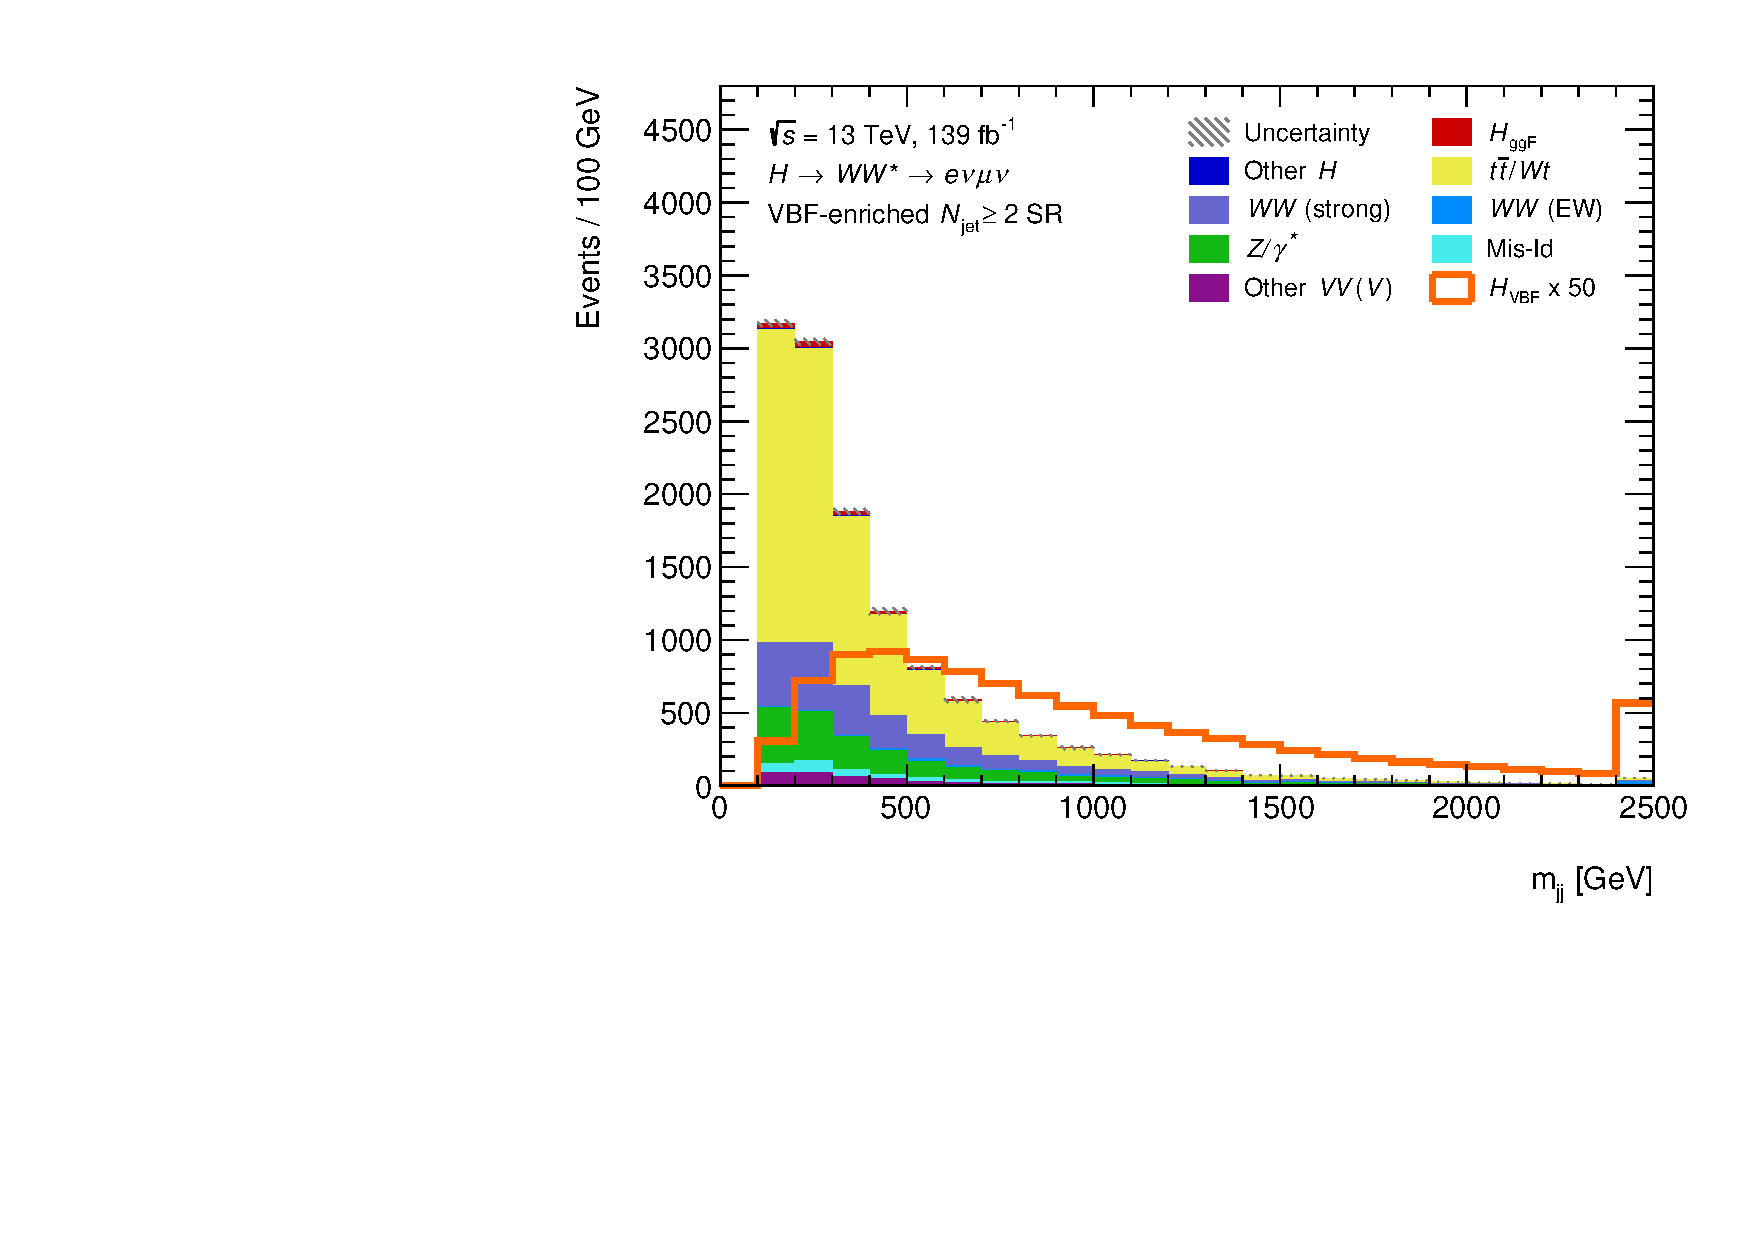
\includegraphics[width=0.32\textwidth]{figures/hww/dnn/blinded/run2-emme-CutVBF_SR-Mjj-lin.pdf} \hfill
        \label{fig:dnn-inputs-post-fit-1}
    } 
    \subfloat[$\dyjj$]{
        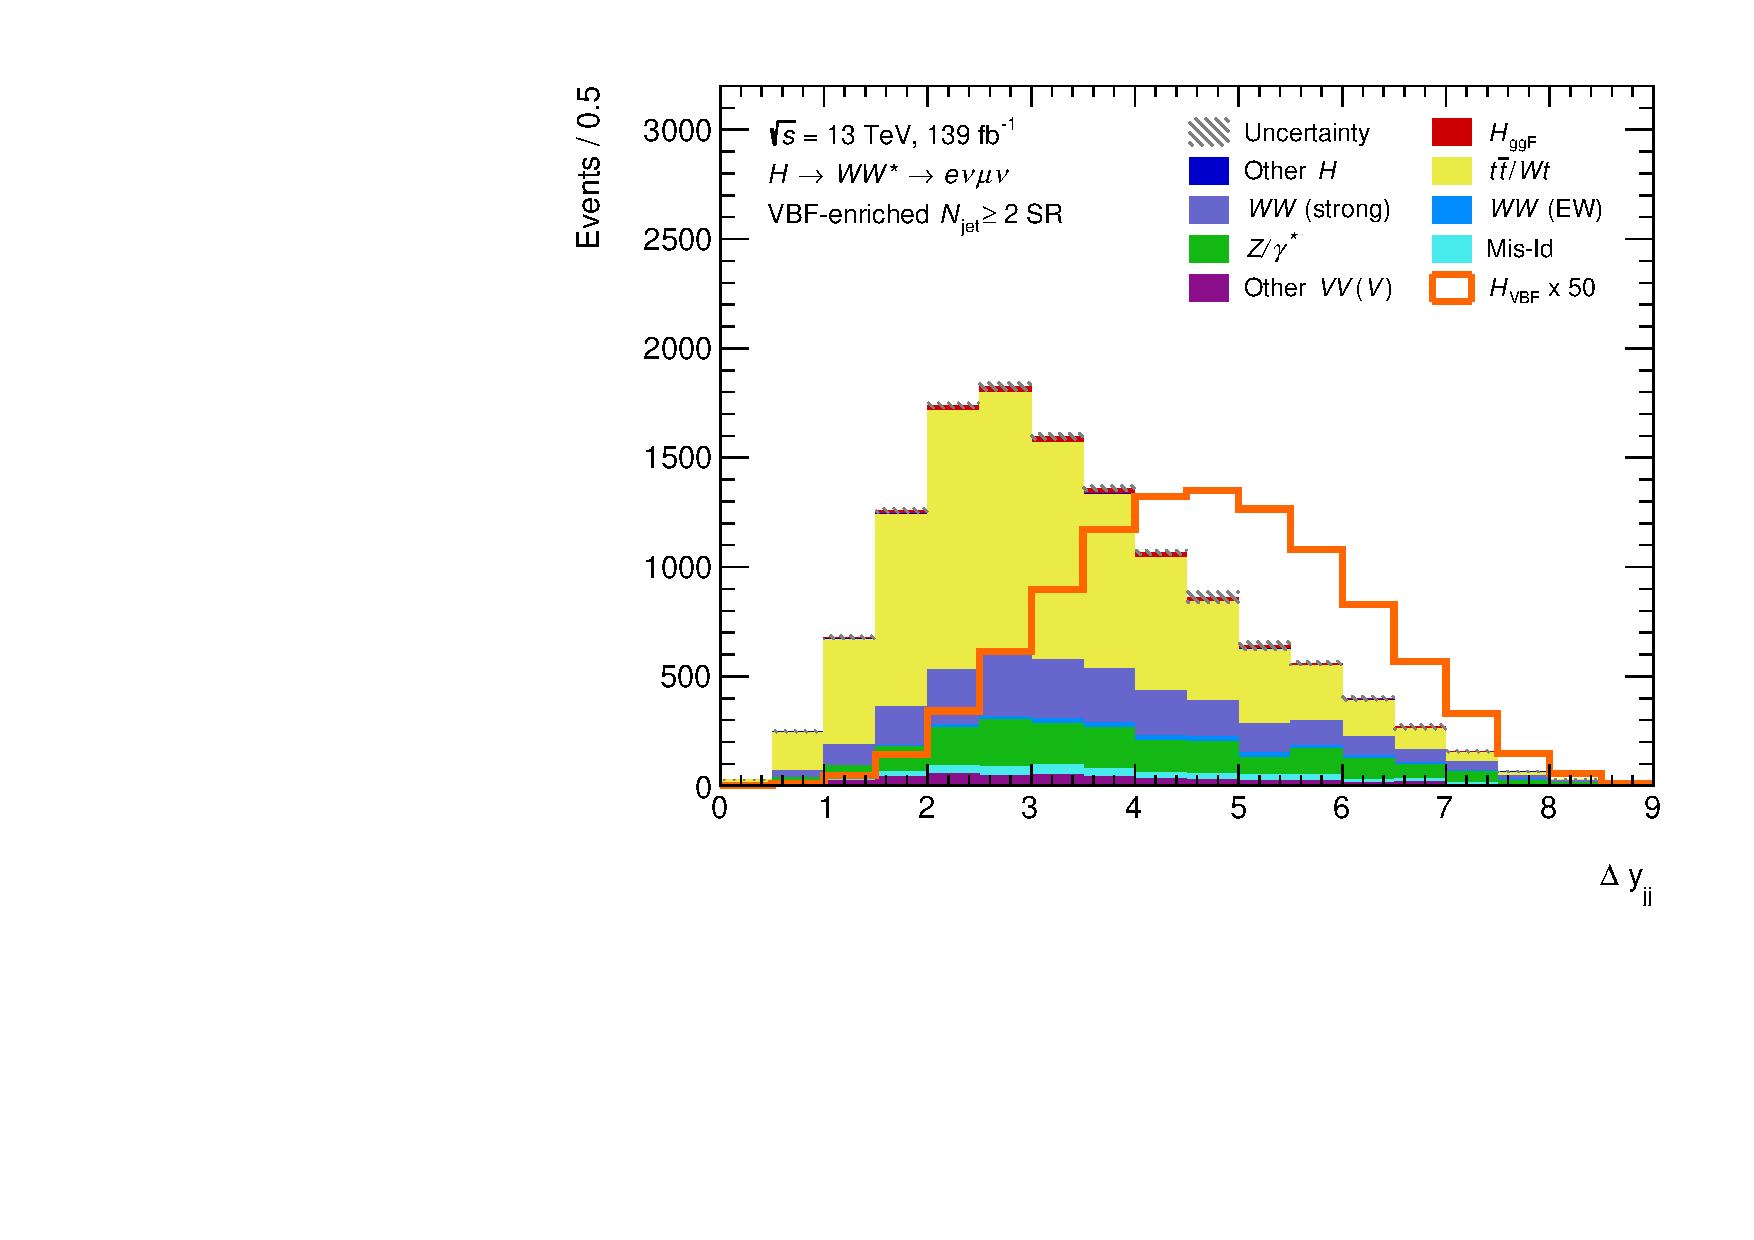
\includegraphics[width=0.32\textwidth]{figures/hww/dnn/blinded/run2-emme-CutVBF_SR-DYjj-lin.pdf} \hfill
        \label{fig:dnn-inputs-post-fit-2}
    } 
    \subfloat[$\lepetacent$]{
        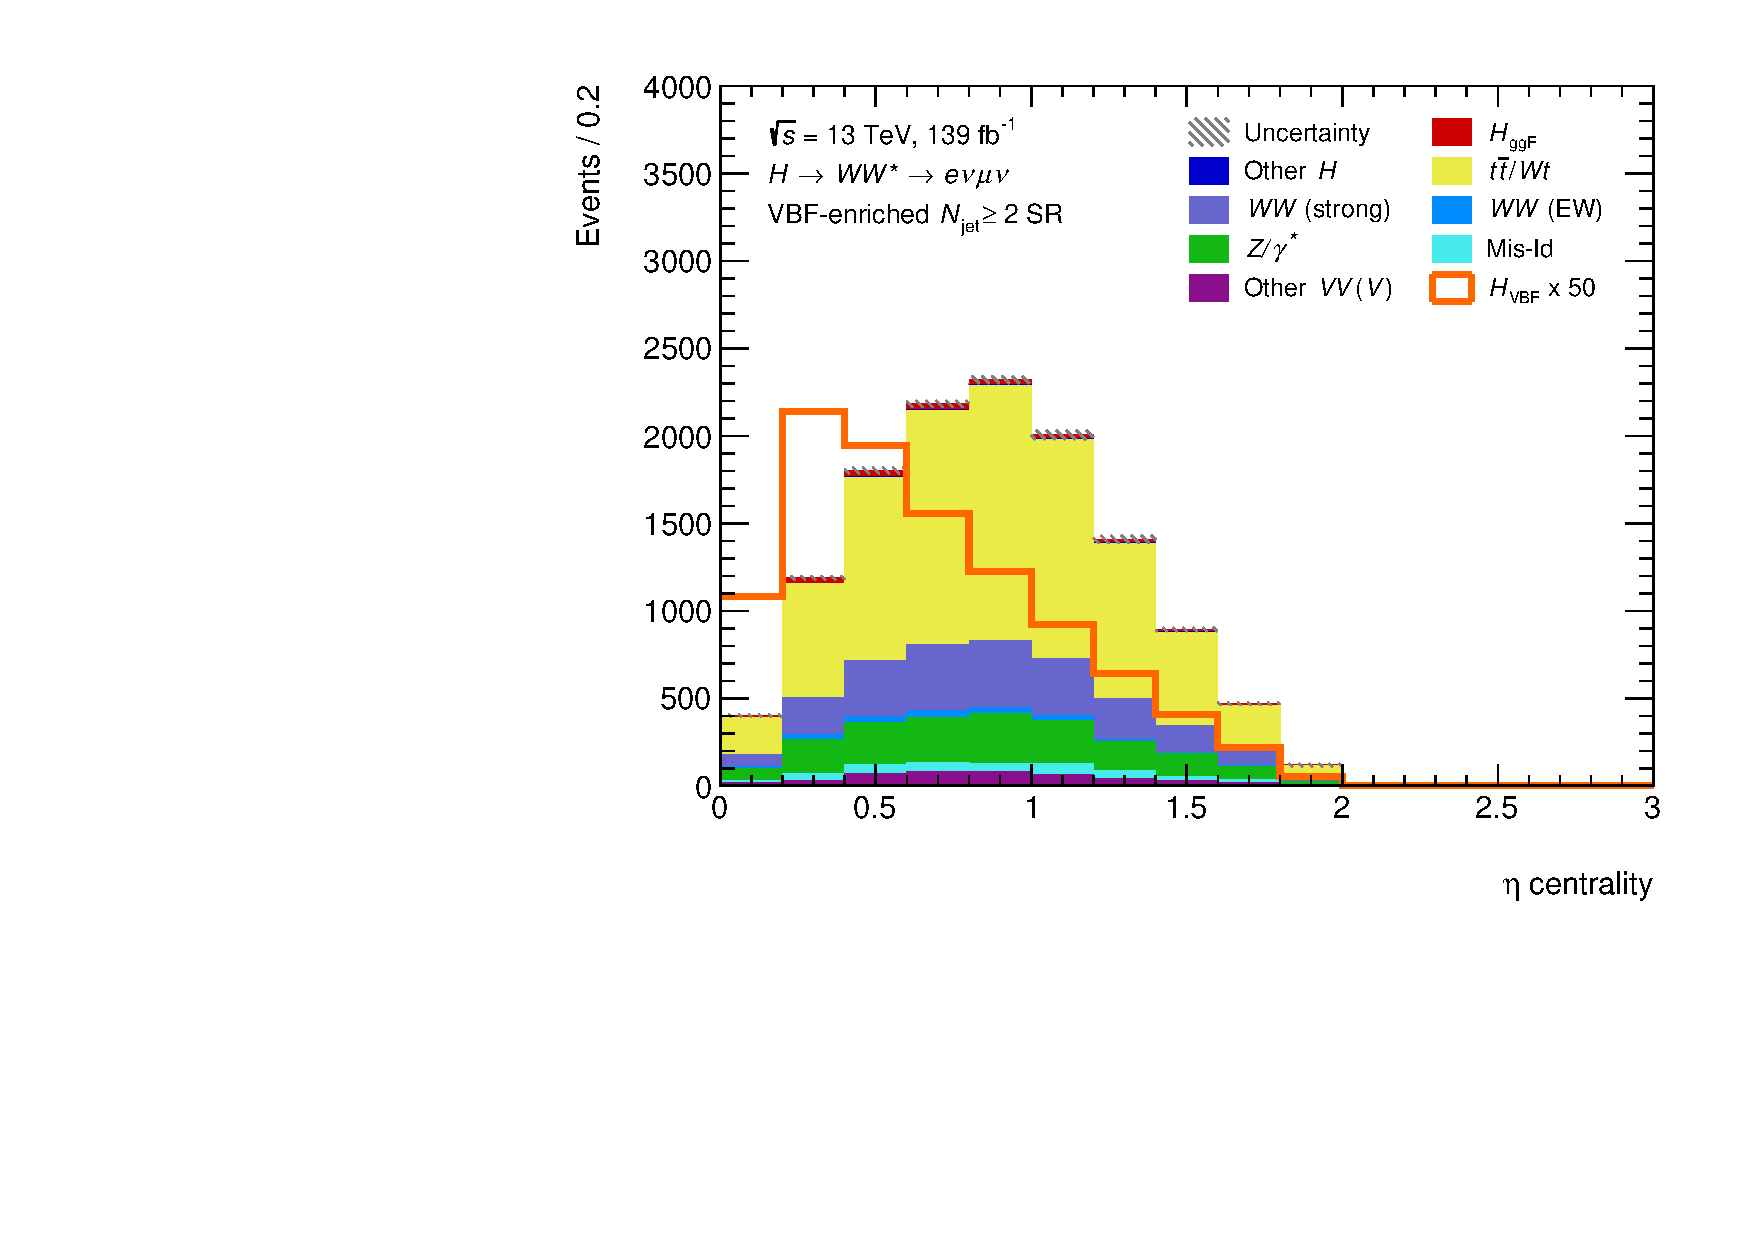
\includegraphics[width=0.32\textwidth]{figures/hww/dnn/blinded/run2-emme-CutVBF_SR-contOLV-lin.pdf} \hfill
        \label{fig:dnn-inputs-post-fit-3}
    } \\
    \subfloat[$\mlonejtwo$]{
        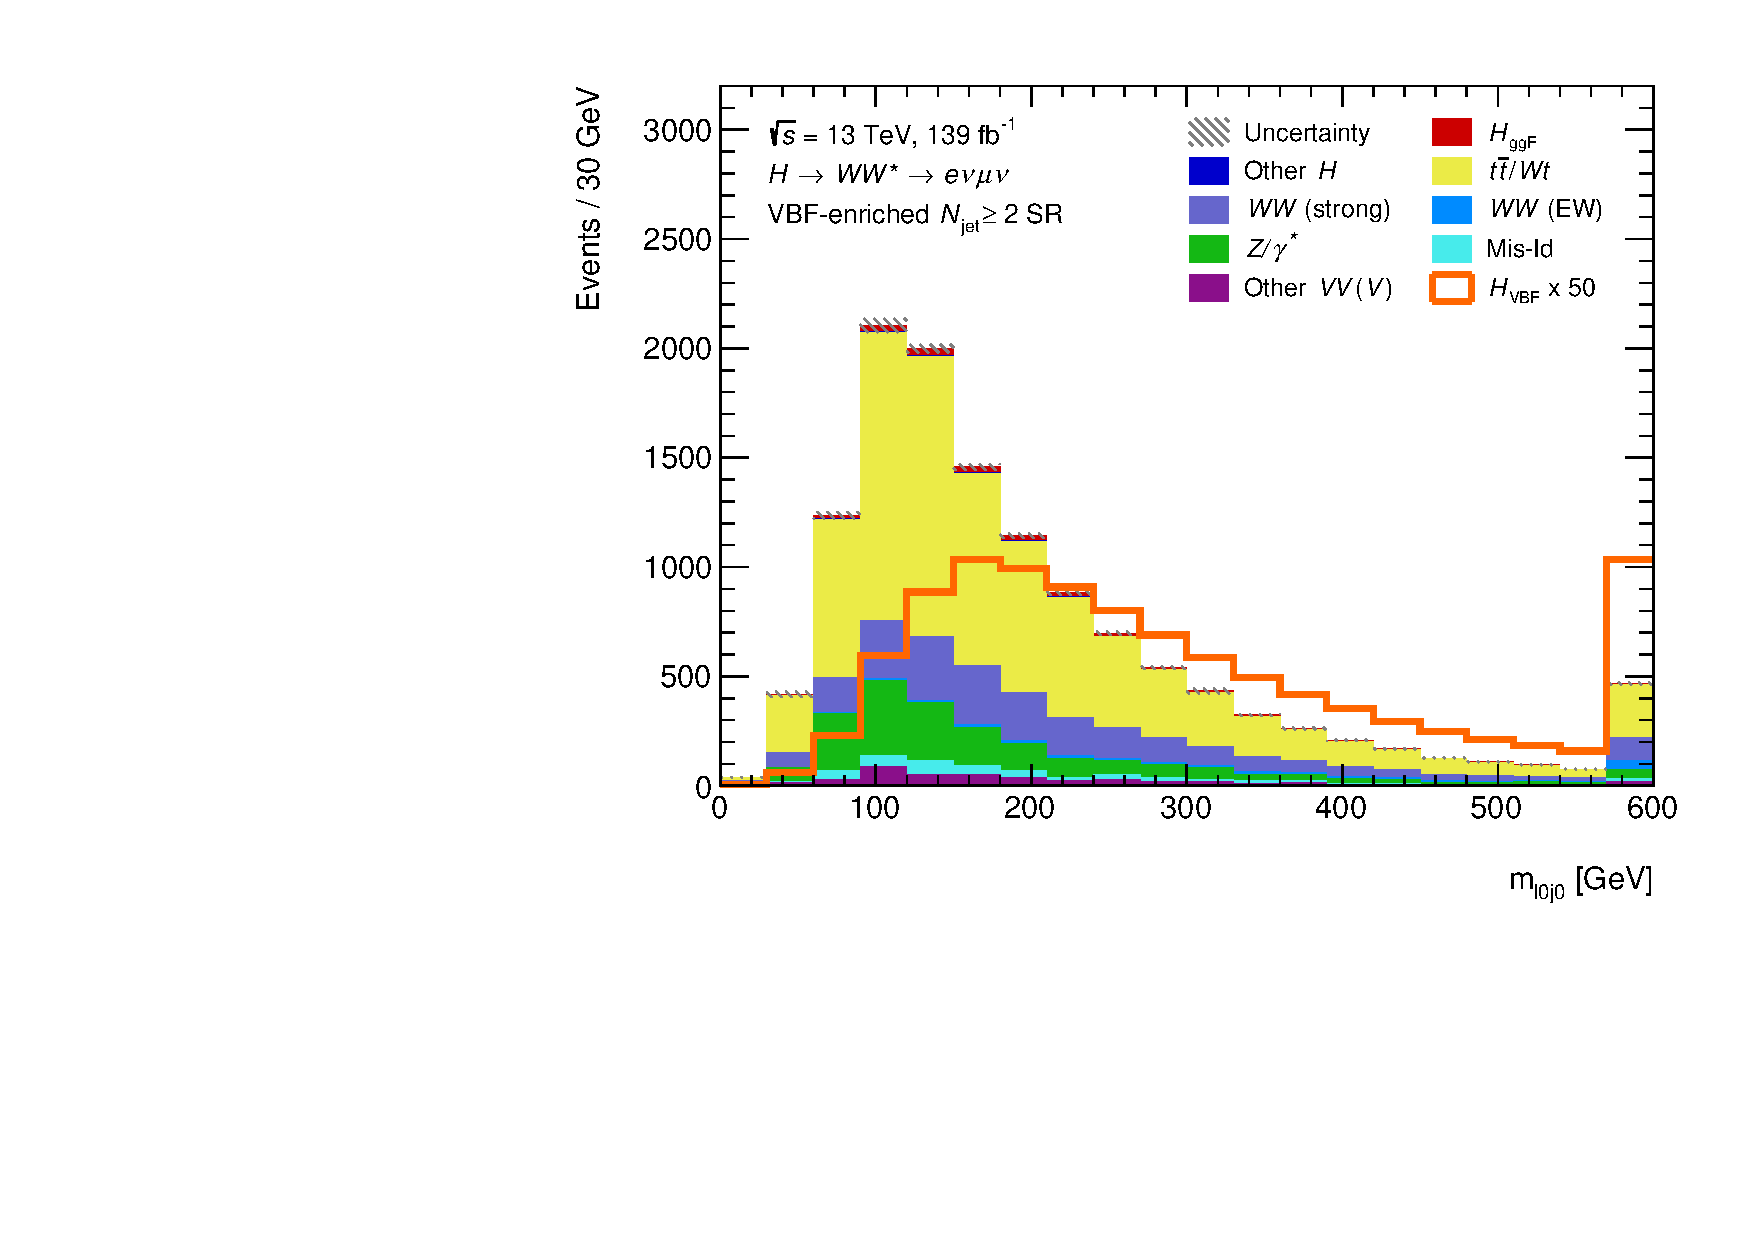
\includegraphics[width=0.32\textwidth]{figures/hww/dnn/blinded/run2-emme-CutVBF_SR-Ml0j0-lin.pdf} \hfill
        \label{fig:dnn-inputs-post-fit-4}
    } 
    \subfloat[$\mltwojone$]{
        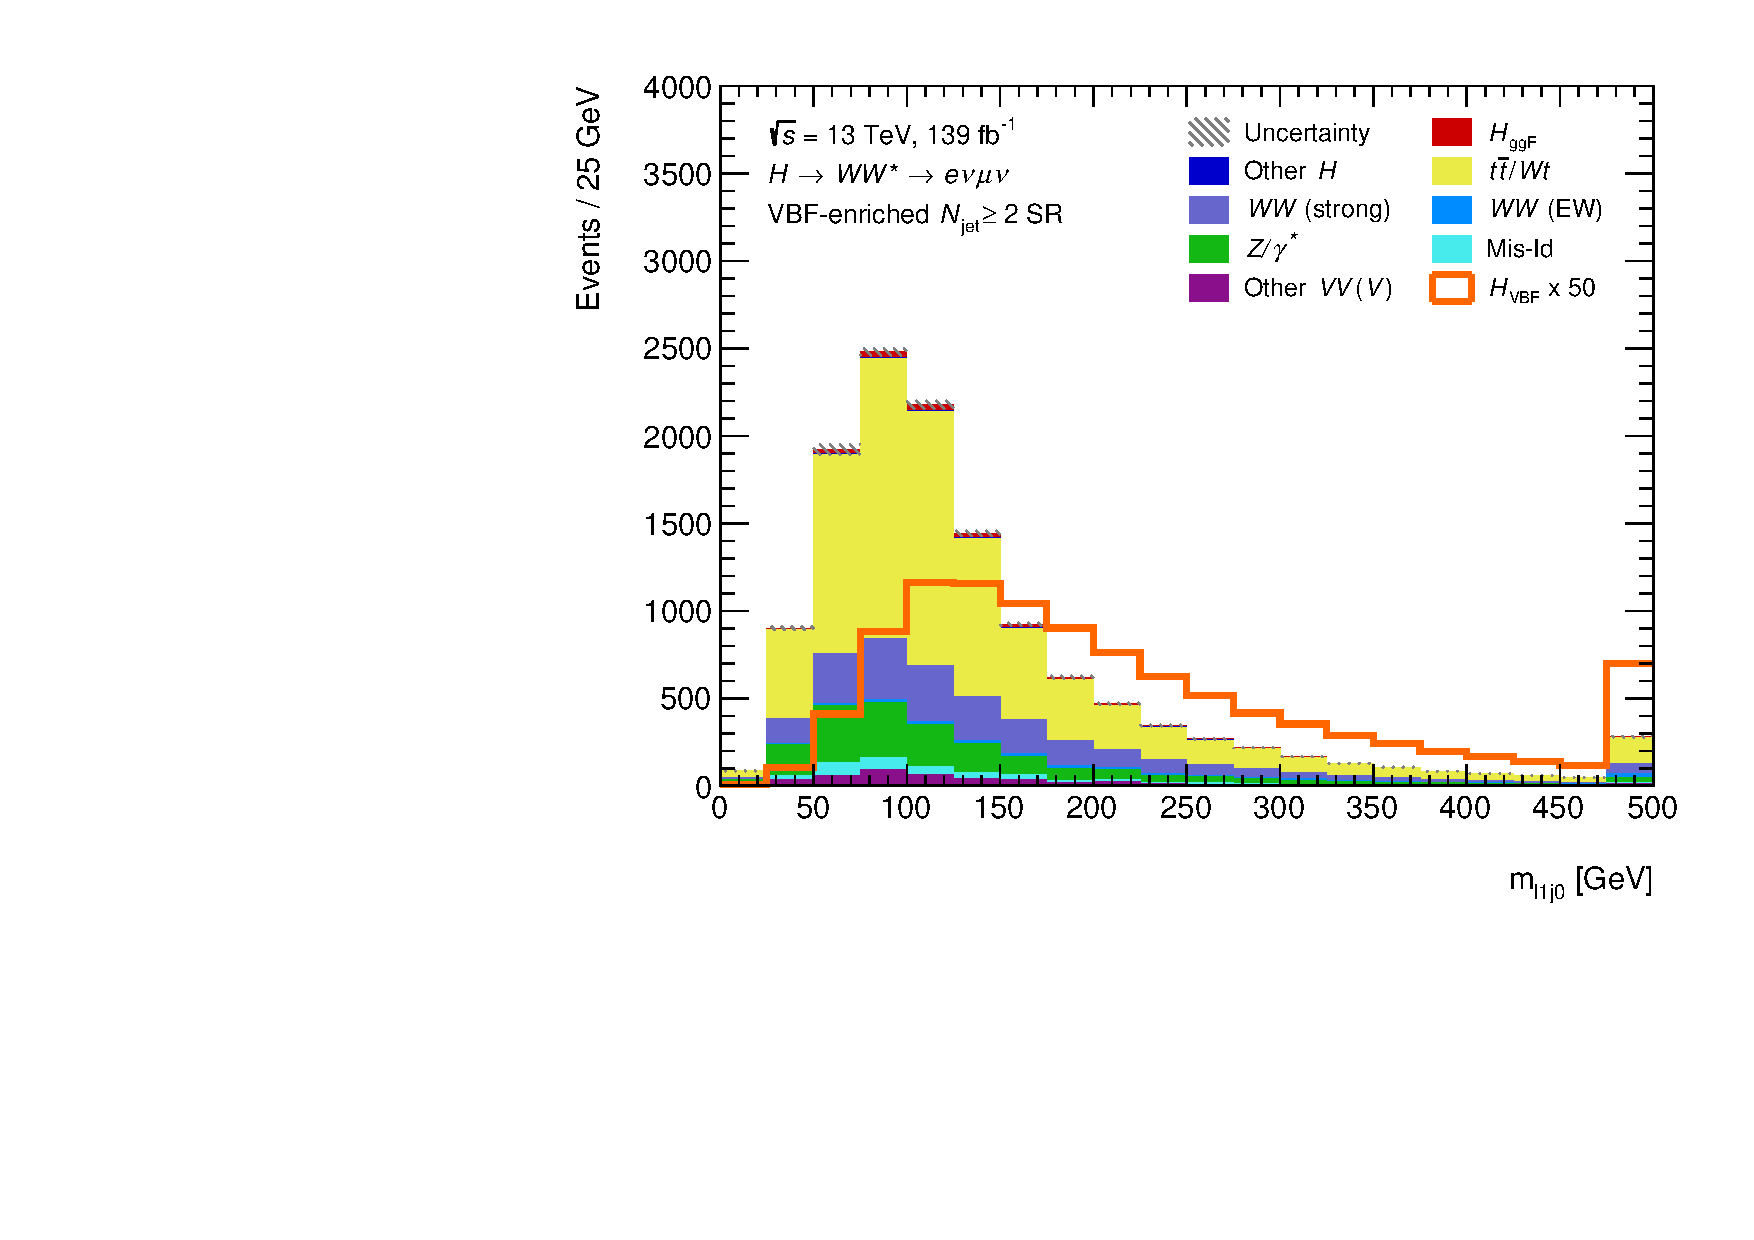
\includegraphics[width=0.32\textwidth]{figures/hww/dnn/blinded/run2-emme-CutVBF_SR-Ml1j0-lin.pdf} \hfill
        \label{fig:dnn-inputs-post-fit-5}
    } 
    \subfloat[$\mlonejtwo$]{
        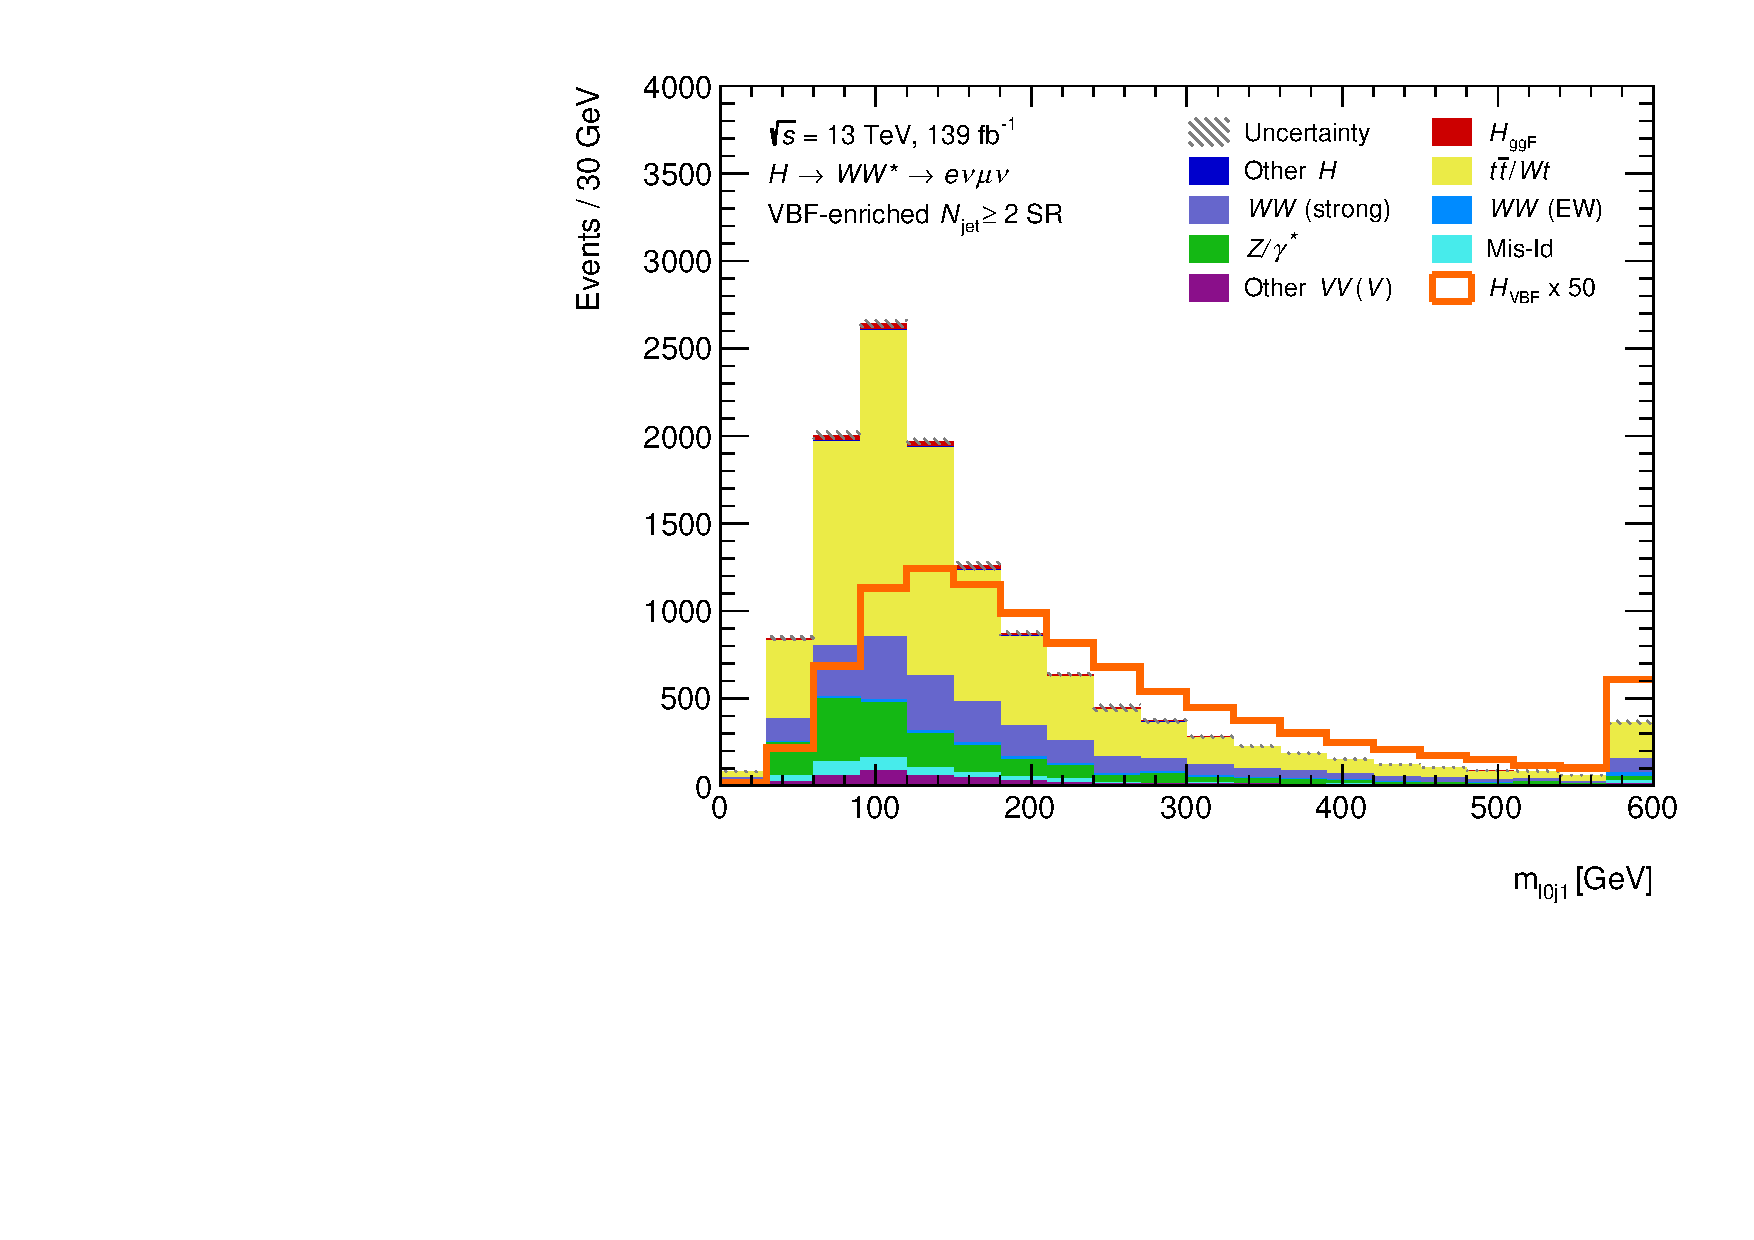
\includegraphics[width=0.32\textwidth]{figures/hww/dnn/blinded/run2-emme-CutVBF_SR-Ml0j1-lin.pdf} \hfill
        \label{fig:dnn-inputs-post-fit-6}
    } \\
    \subfloat[$\mltwojtwo$]{
        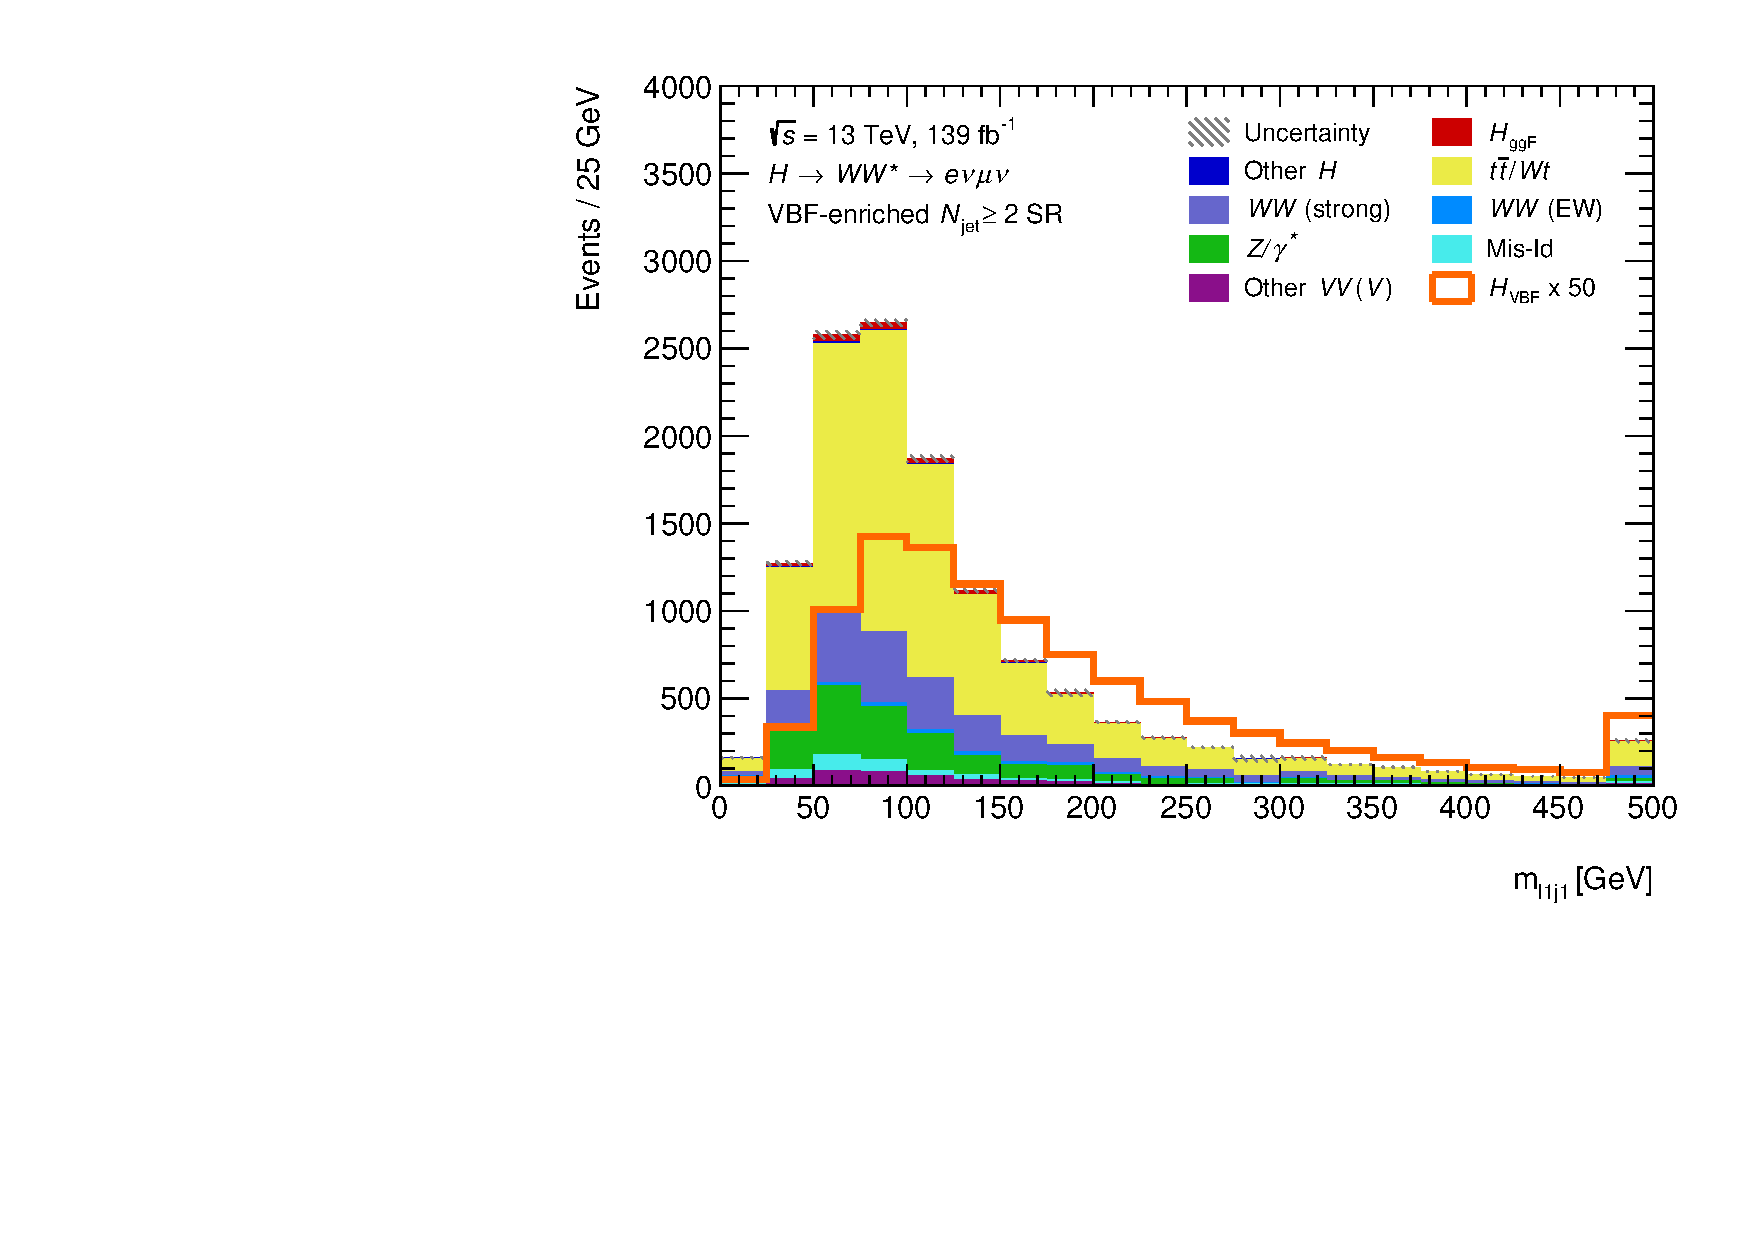
\includegraphics[width=0.32\textwidth]{figures/hww/dnn/blinded/run2-emme-CutVBF_SR-Ml1j1-lin.pdf} \hfill
        \label{fig:dnn-inputs-post-fit-7}
    } 
    \subfloat[$\pTjone$]{
        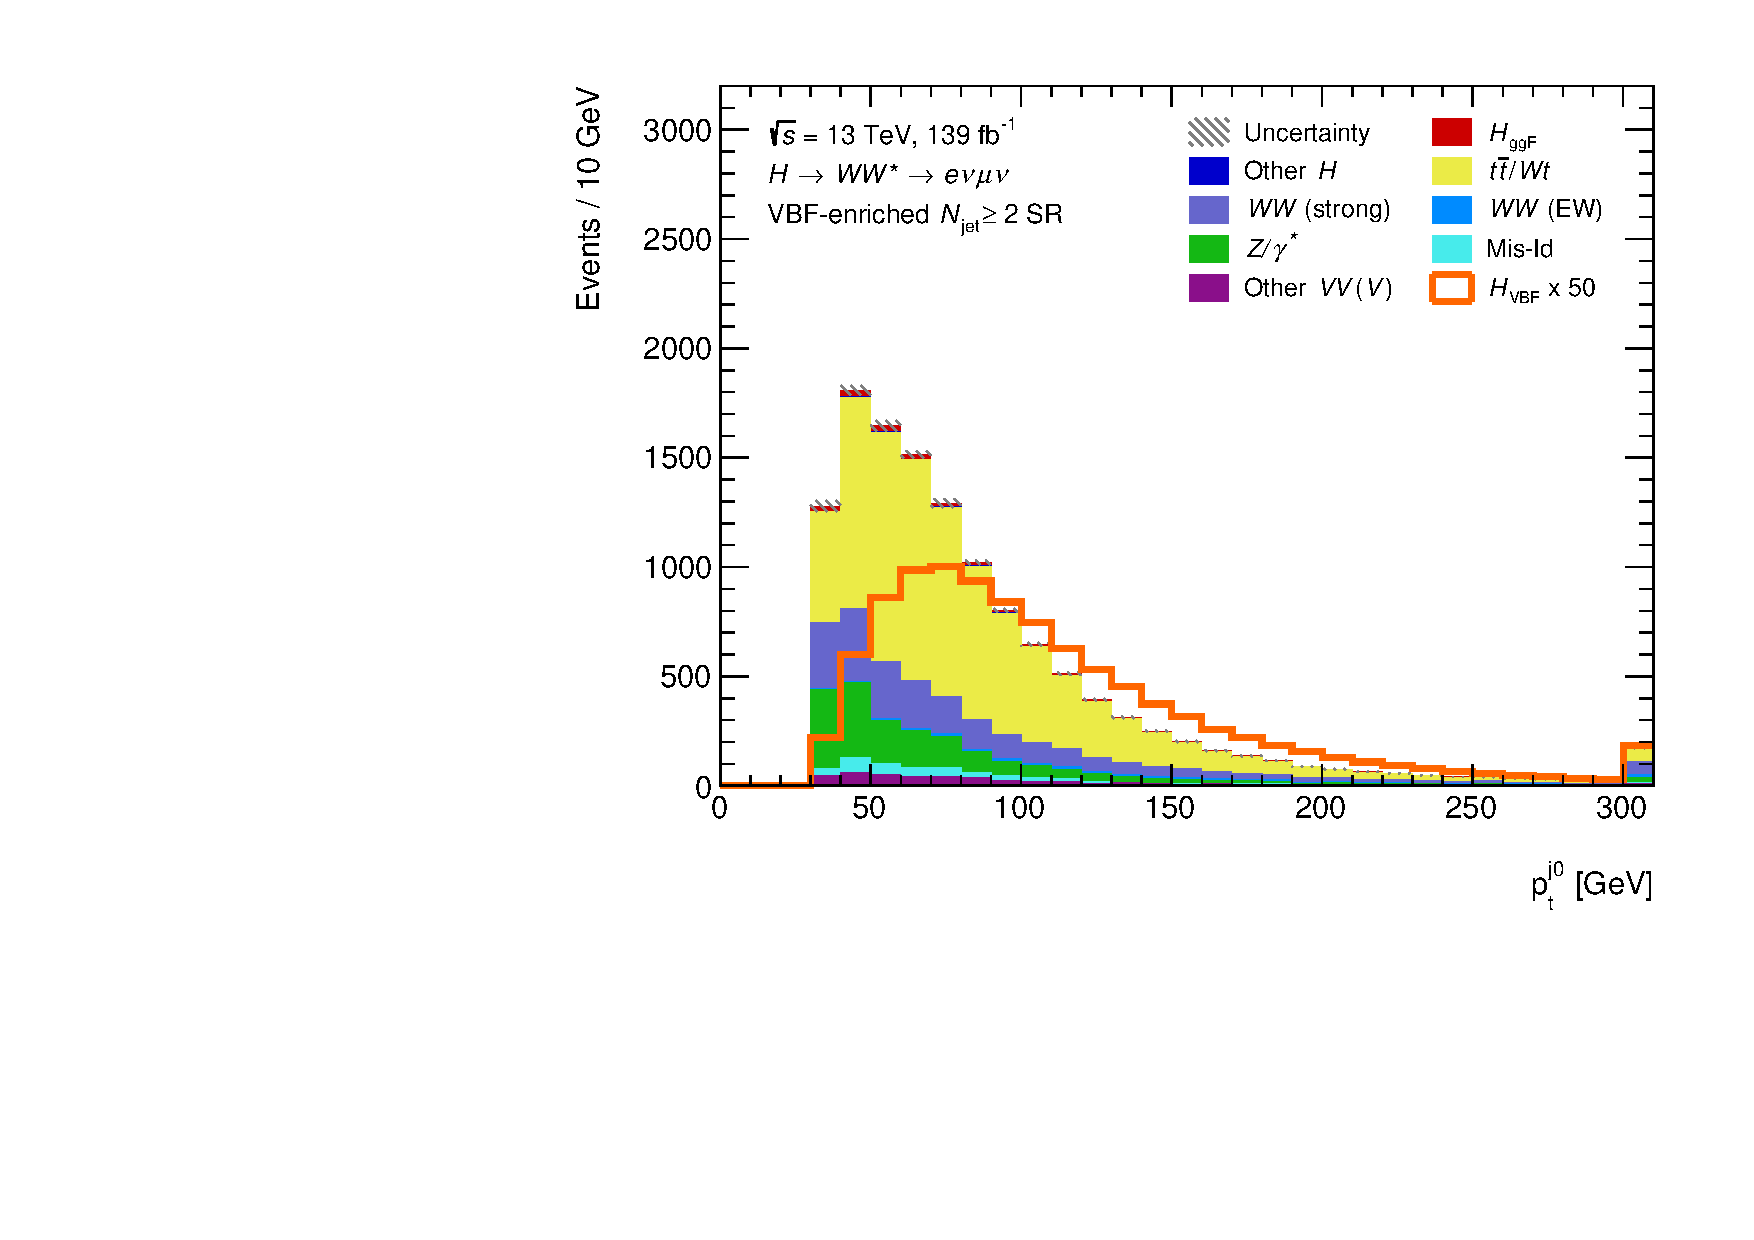
\includegraphics[width=0.32\textwidth]{figures/hww/dnn/blinded/run2-emme-CutVBF_SR-leadJetPt-lin.pdf} \hfill
        \label{fig:dnn-inputs-post-fit-8}
    } 
    \subfloat[$\pTjtwo$]{
        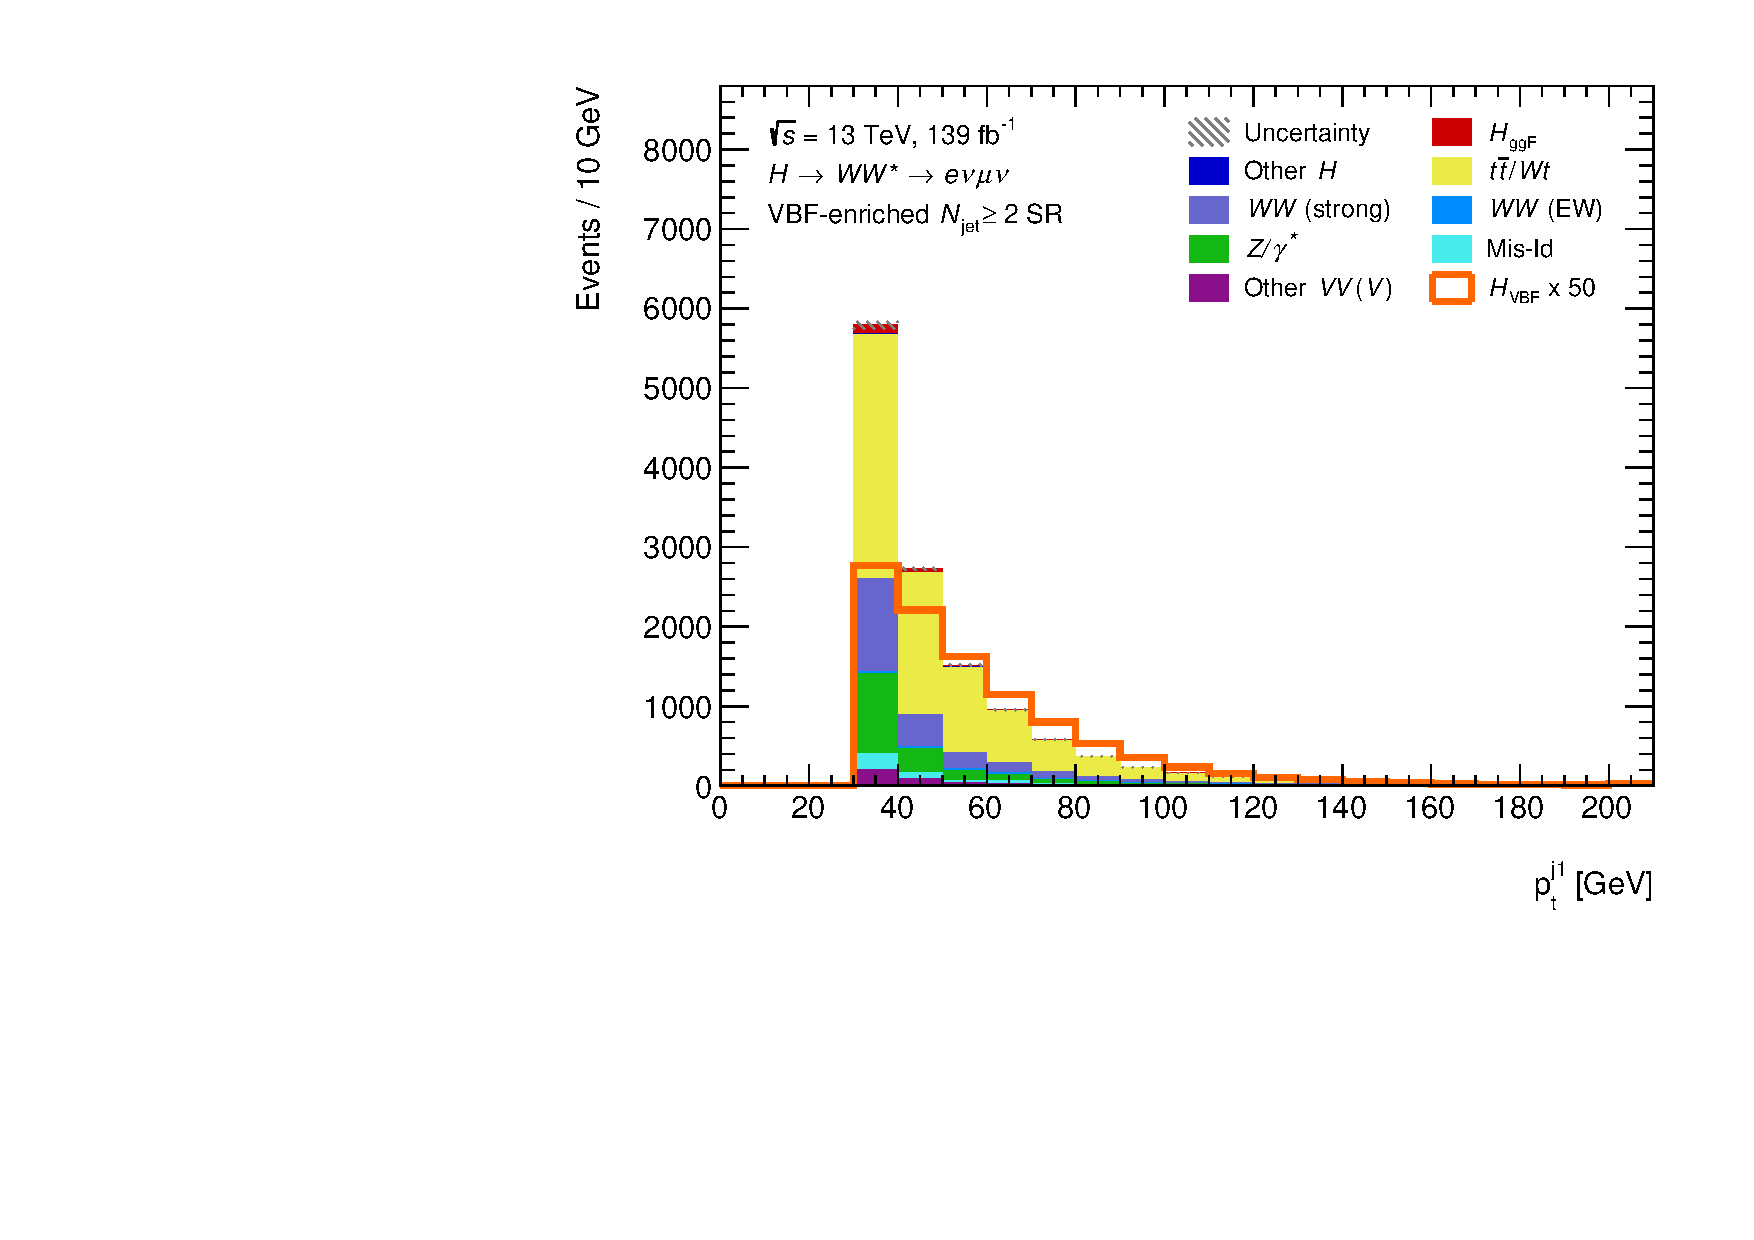
\includegraphics[width=0.32\textwidth]{figures/hww/dnn/blinded/run2-emme-CutVBF_SR-subleadJetPt-lin.pdf} \hfill
        \label{fig:dnn-inputs-post-fit-9}
    } \\
    \subfloat[$\pTjthree$]{
        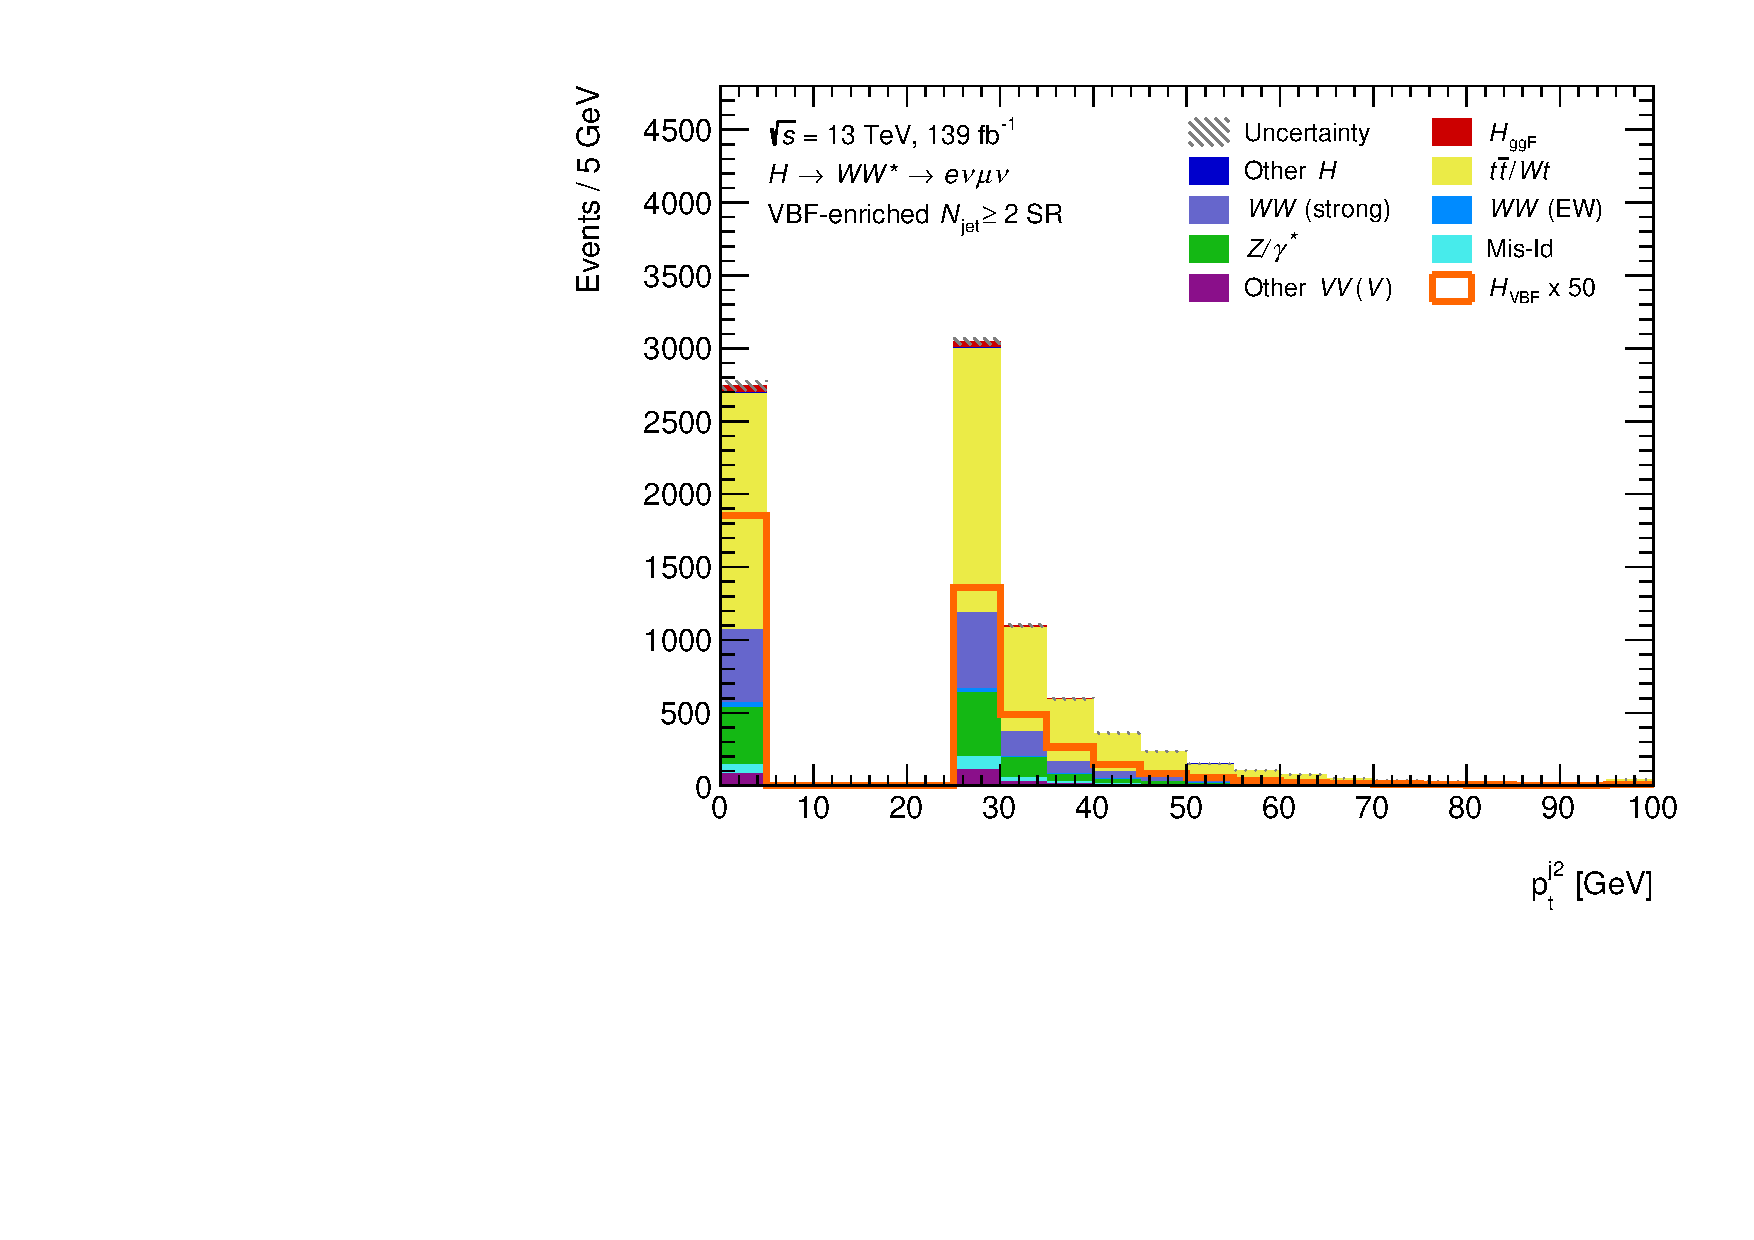
\includegraphics[width=0.32\textwidth]{figures/hww/dnn/blinded/run2-emme-CutVBF_SR-thirdJetPt-lin.pdf} \hfill
        \label{fig:dnn-inputs-post-fit-10}
    } 
    {\caption{Distributions of $\dphill$, $\mll$, $\lepetacent$, \pTjone, \pTjtwo, \pTjthree in the VBF signal region.
        Each row corresponds to one variable with different selections made on the DNN output.
        \label{fig:dnn-inputs-post-fit1} }}
\end{figure}


% \begin{figure}[h]
%     \centering
%     {\caption{Distributions of $\mlonejone$, $\mltwojone$, $\mlonejtwo$, and $\mltwojtwo$ in the VBF signal region.
%             Each row shows one variable with different cuts on the DNN output distribution being applied in different columns.
%             \label{app:fig:dnn-inputs-vbf-top2} }}
% \end{figure}


\begin{figure}[h]
    \centering
    \subfloat[$\dphill$]{
        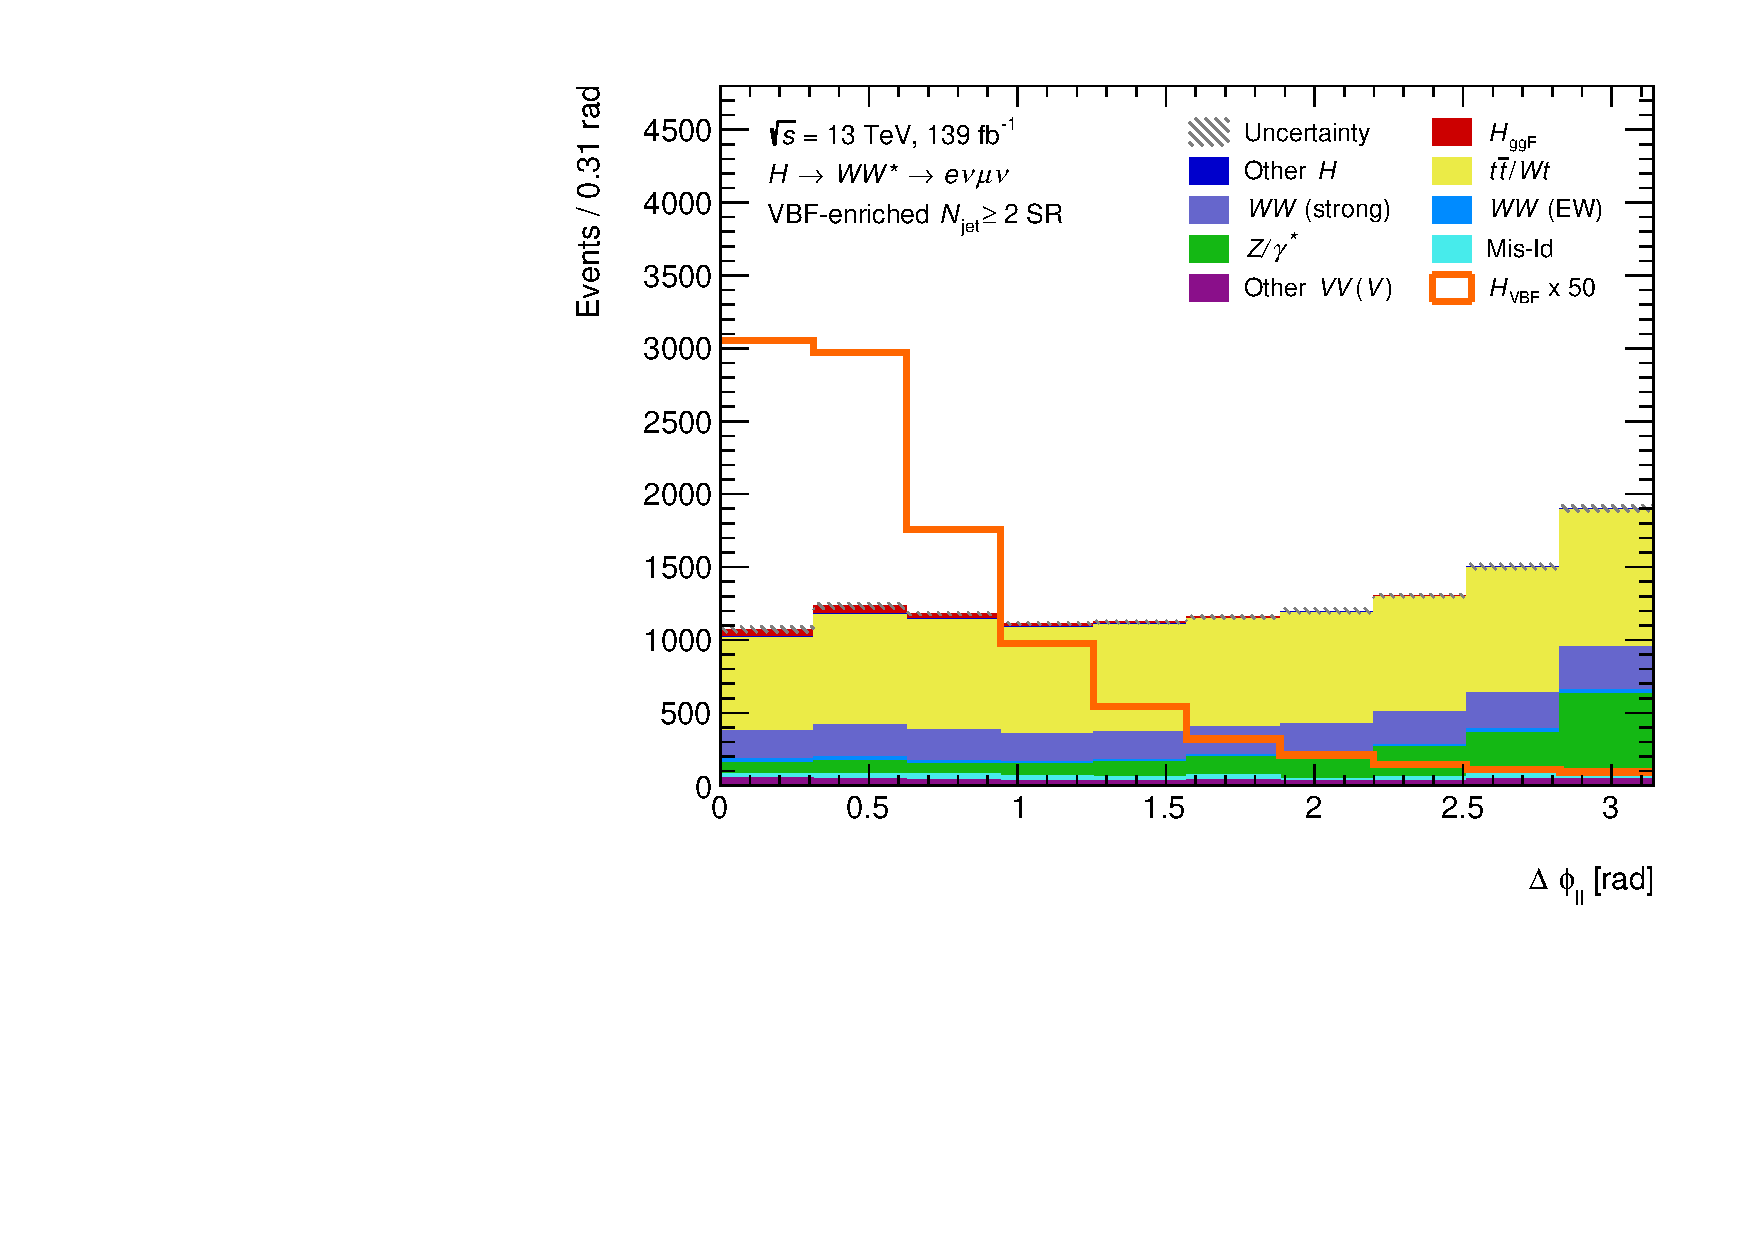
\includegraphics[width=0.32\textwidth]{figures/hww/dnn/blinded/run2-emme-CutVBF_SR-DPhill-lin.pdf} \hfill
        \label{fig:dnn-inputs-post-fit2-1}
    } 
    \subfloat[$\mll$]{
        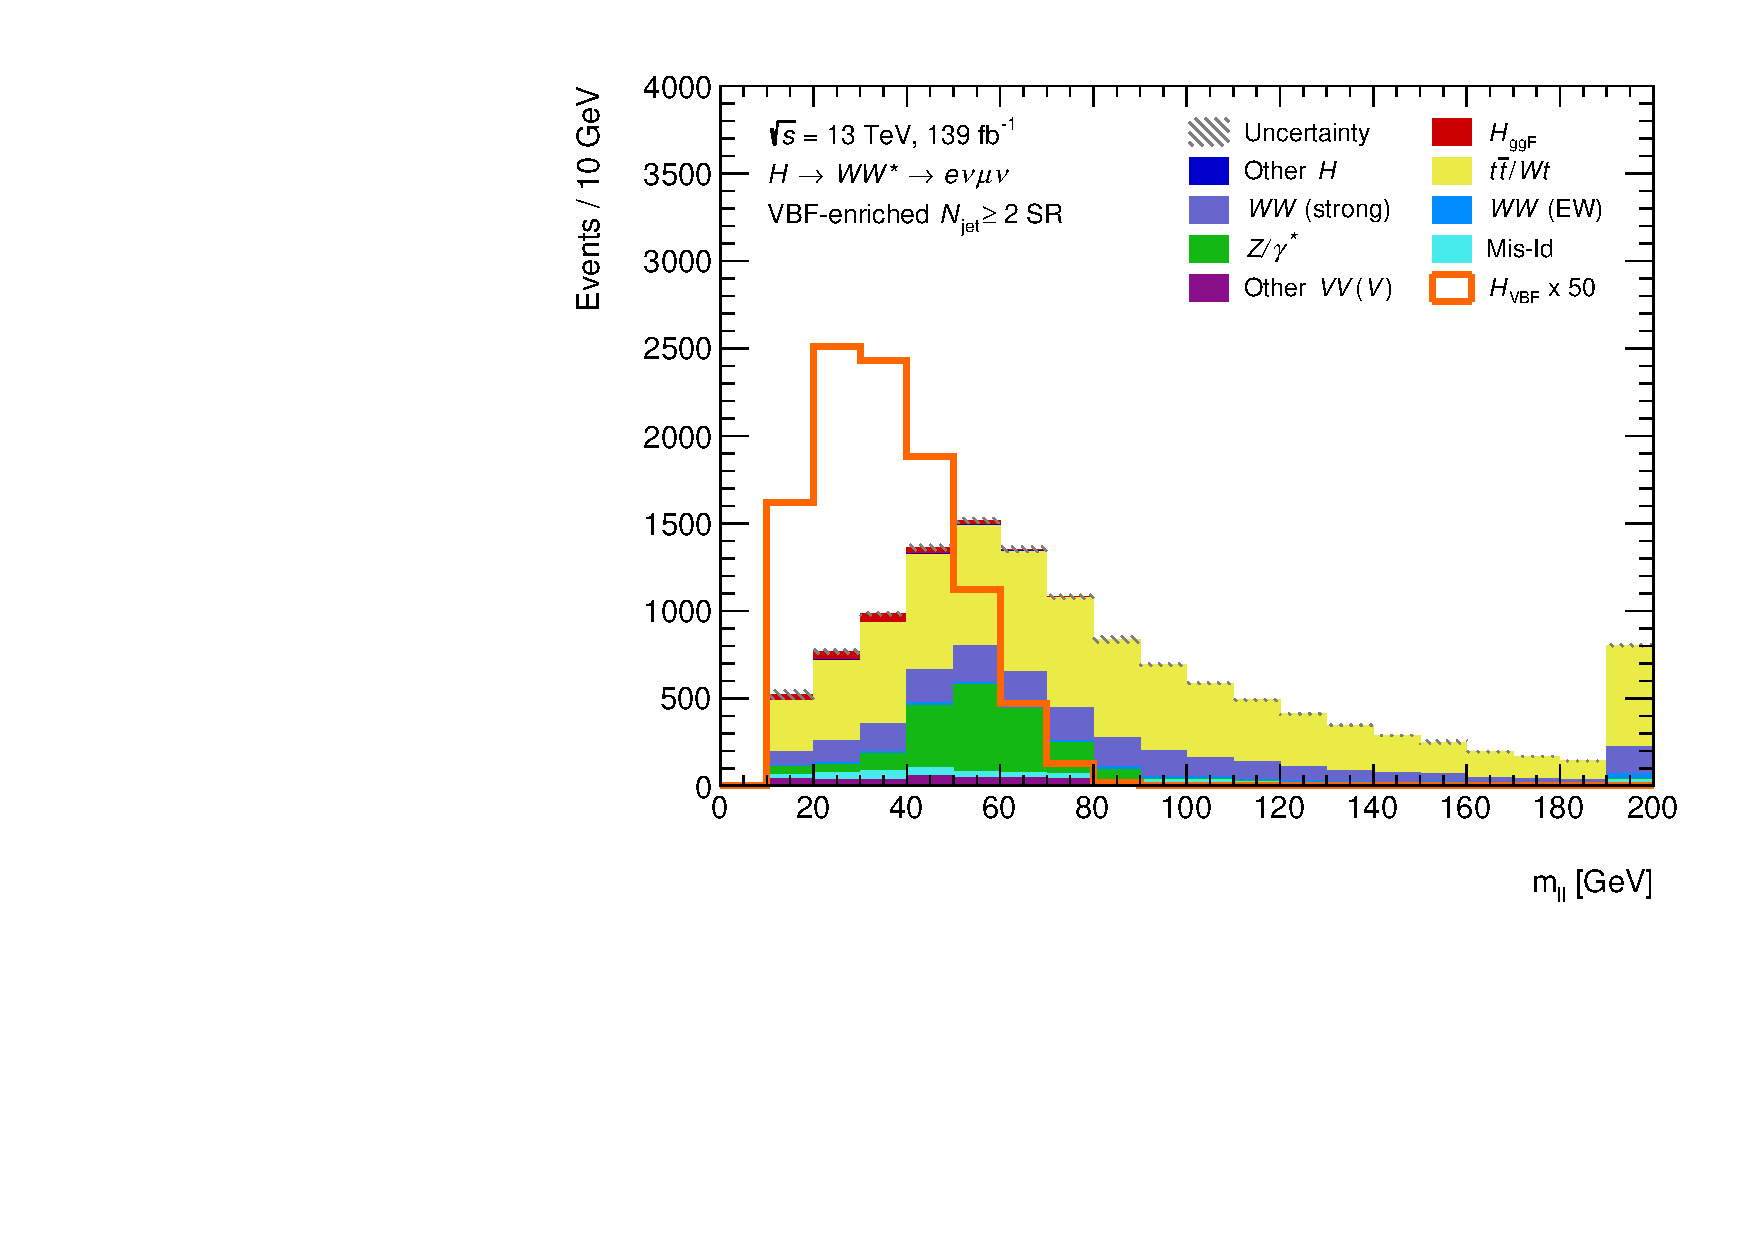
\includegraphics[width=0.32\textwidth]{figures/hww/dnn/blinded/run2-emme-CutVBF_SR-Mll-lin.pdf}
        \label{fig:dnn-inputs-post-fit2-2}
    } 
    \subfloat[$\mT$]{
        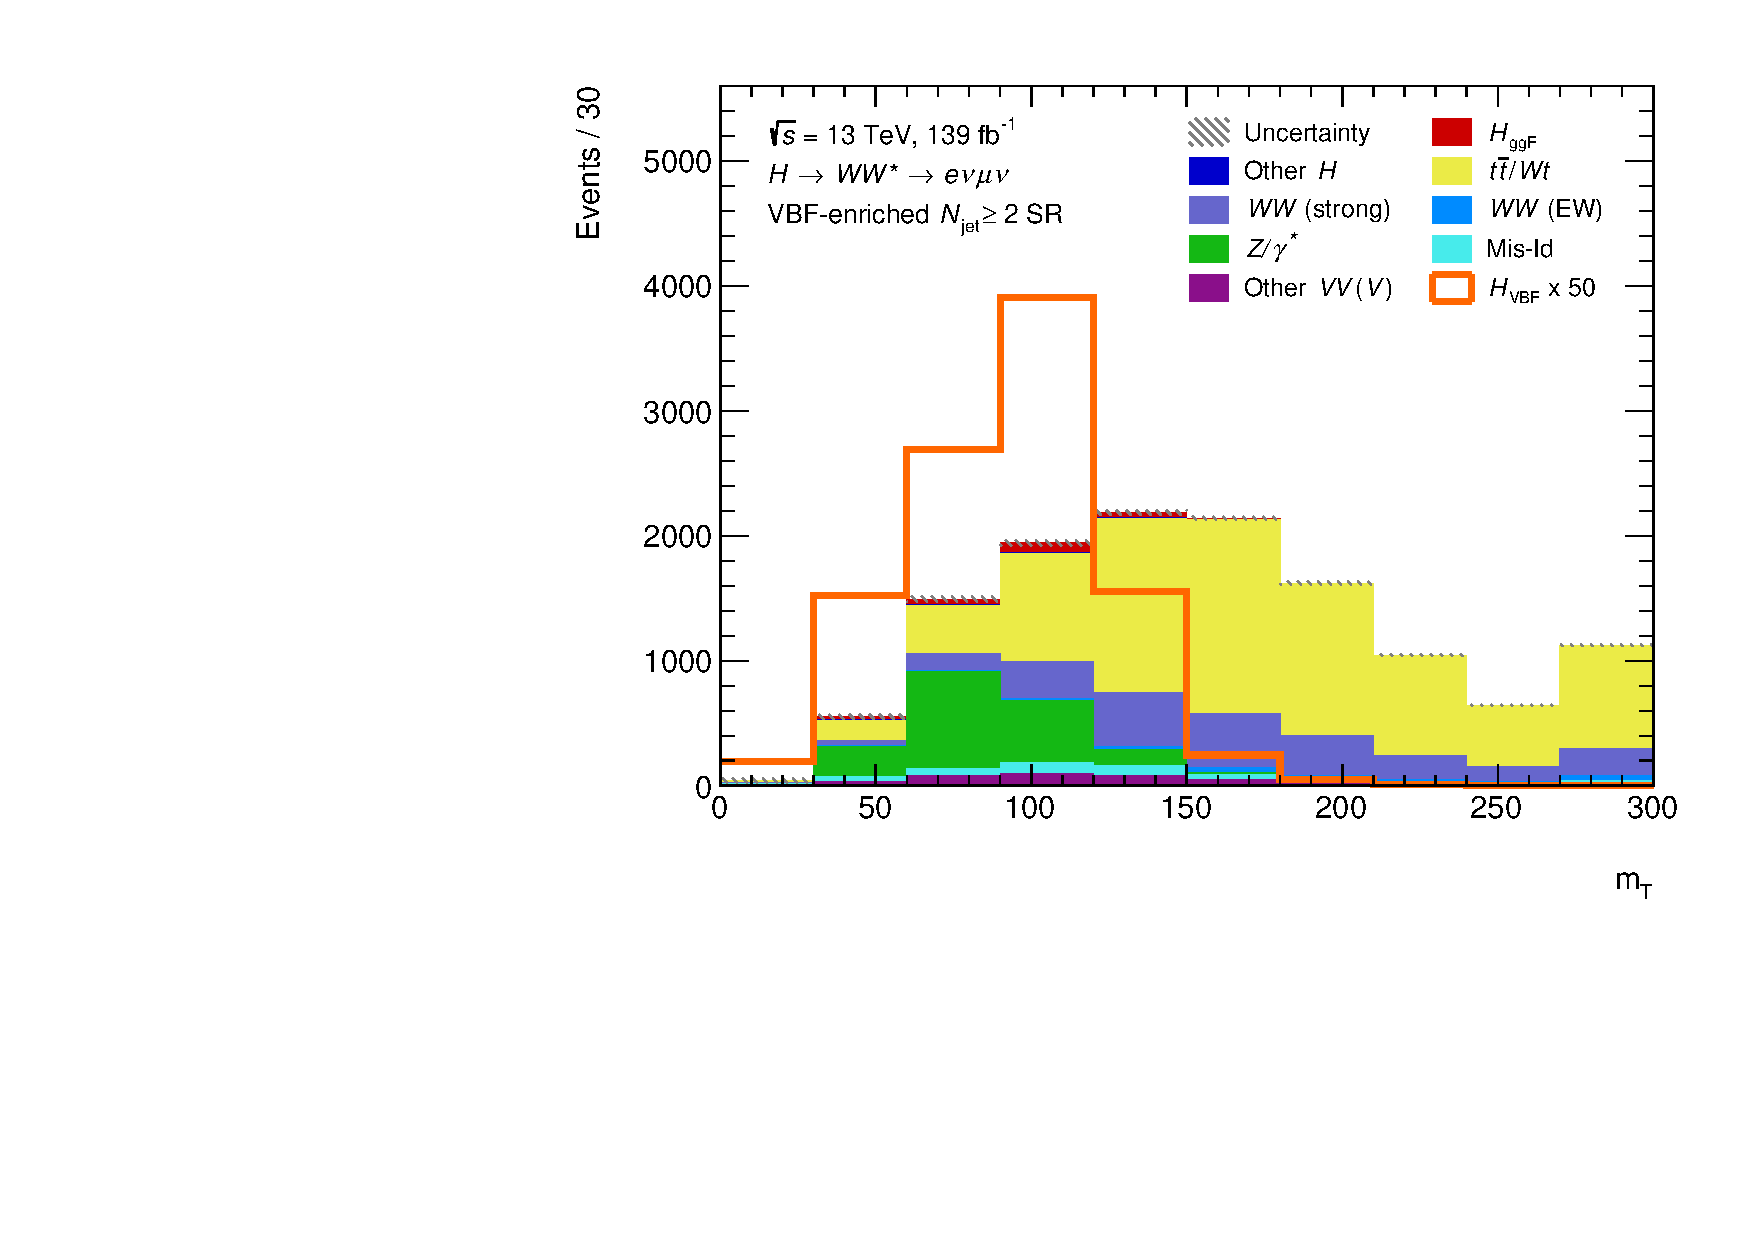
\includegraphics[width=0.32\textwidth]{figures/hww/dnn/blinded/run2-emme-CutVBF_SR-MT-lin.pdf} \hfill
        \label{fig:dnn-inputs-post-fit2-3}
    } \\
    \subfloat[$\pttot$]{
        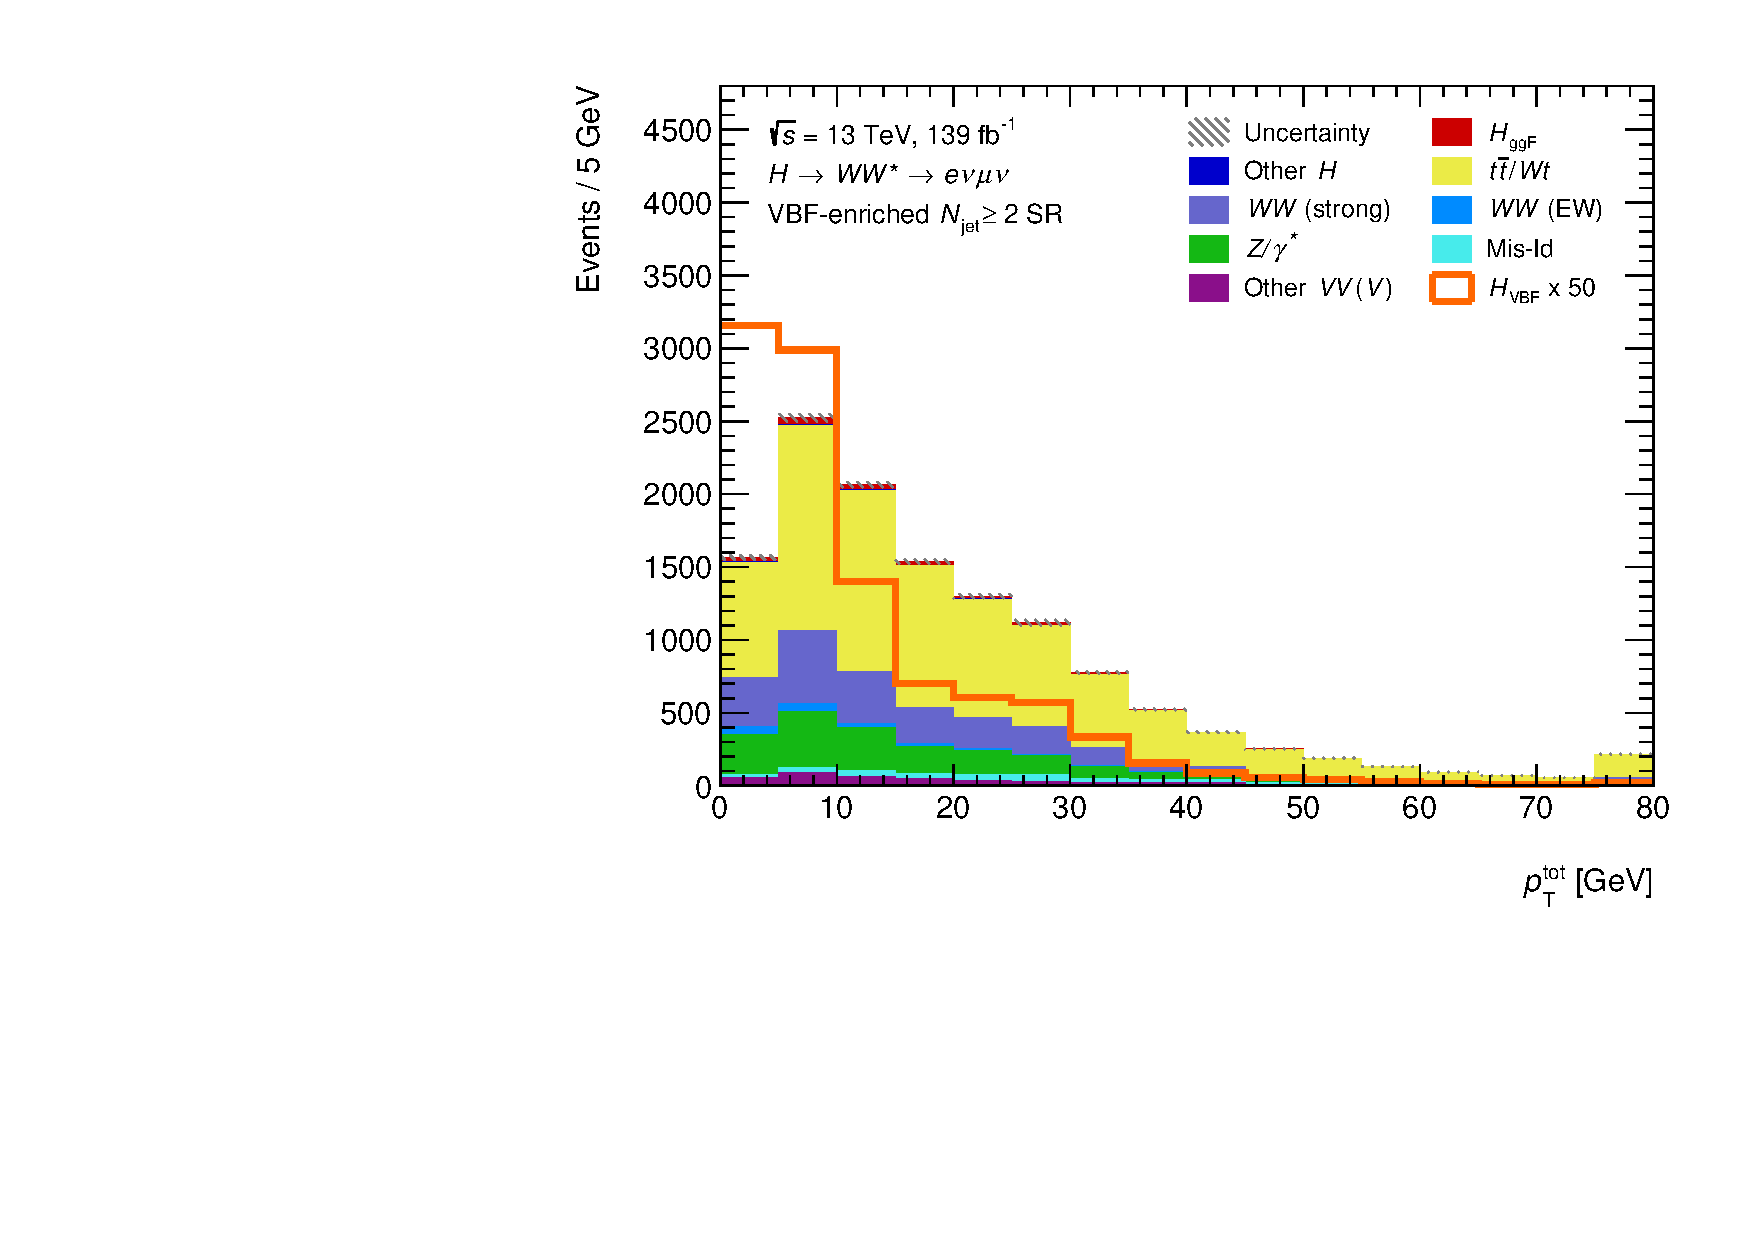
\includegraphics[width=0.32\textwidth]{figures/hww/dnn/blinded/run2-emme-CutVBF_SR-PtTot-lin.pdf} \hfill
        \label{fig:dnn-inputs-post-fit2-4}
    } 
    \subfloat[$\METSig$]{
        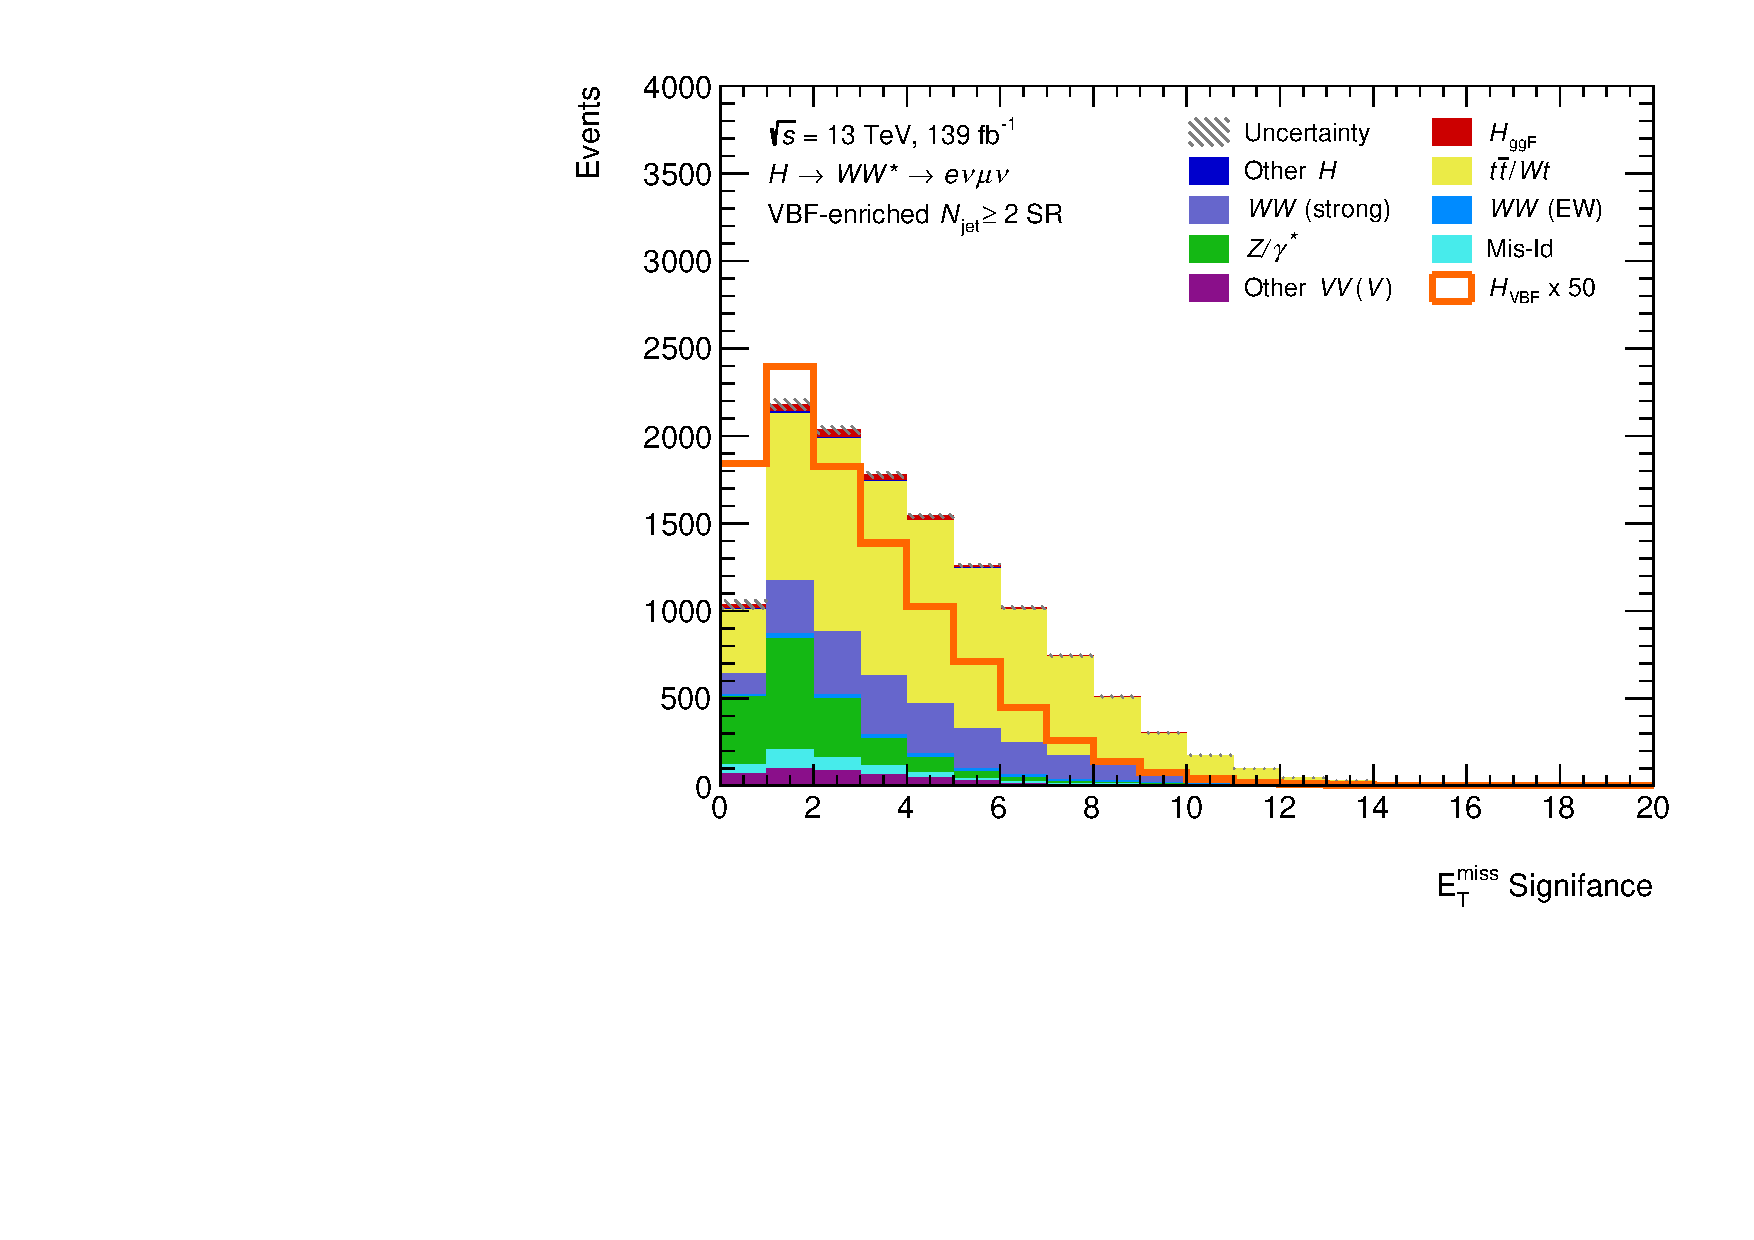
\includegraphics[width=0.32\textwidth]{figures/hww/dnn/blinded/run2-emme-CutVBF_SR-METSig_broad-lin.pdf} \hfill
        \label{fig:dnn-inputs-post-fit2-5}
    } 
    {\caption{Distributions of $\dphill$, $\mll$, $\mT$ in the VBF signal region.
        Each row corresponds to one variable with different selections made on the DNN output.
        \label{fig:dnn-inputs-post-fit2} }}
\end{figure}
}


\newcommand{\dnnfigures}{
\begin{figure}[h]
    \centering
    \subfloat[$\mjj$]{
        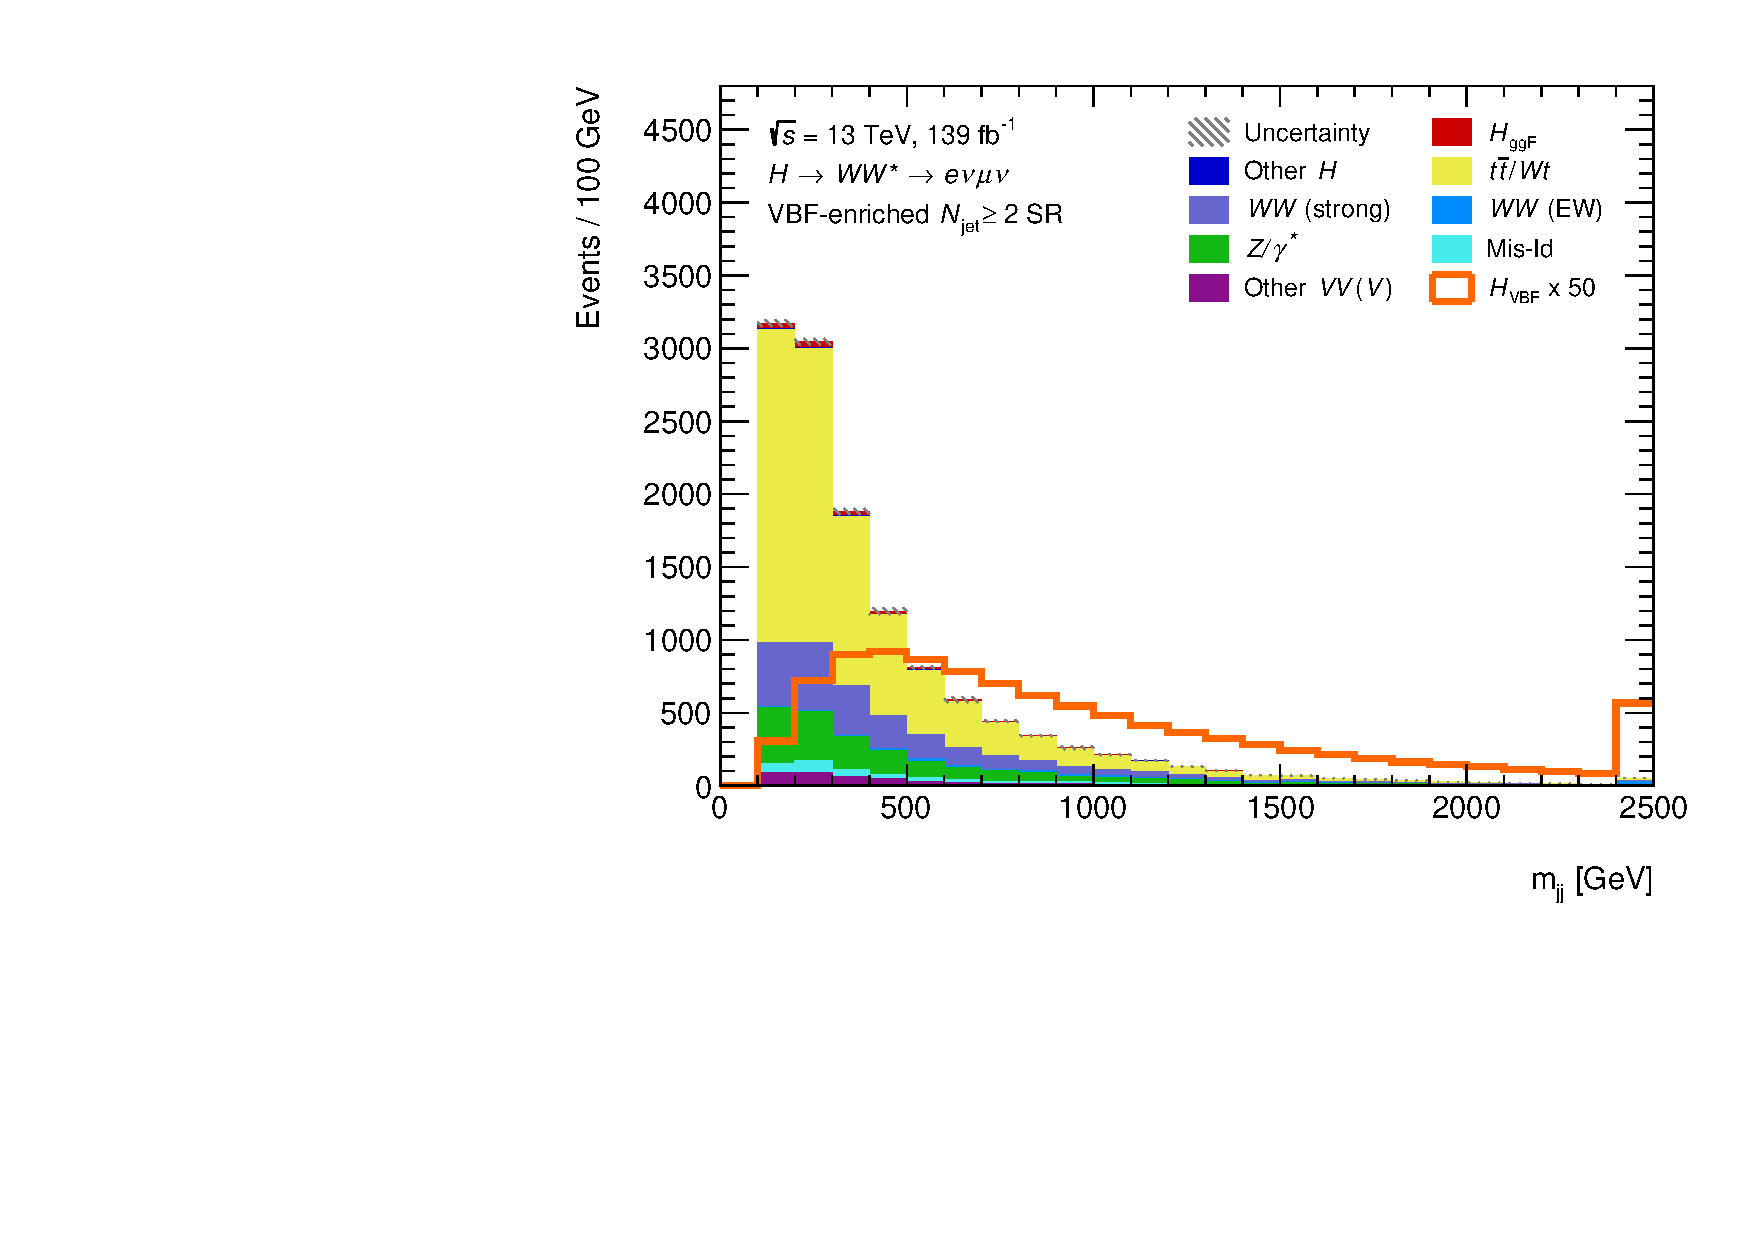
\includegraphics[width=0.32\textwidth]{figures/hww/dnn/blinded/run2-emme-CutVBF_SR-Mjj-lin.pdf} \hfill
        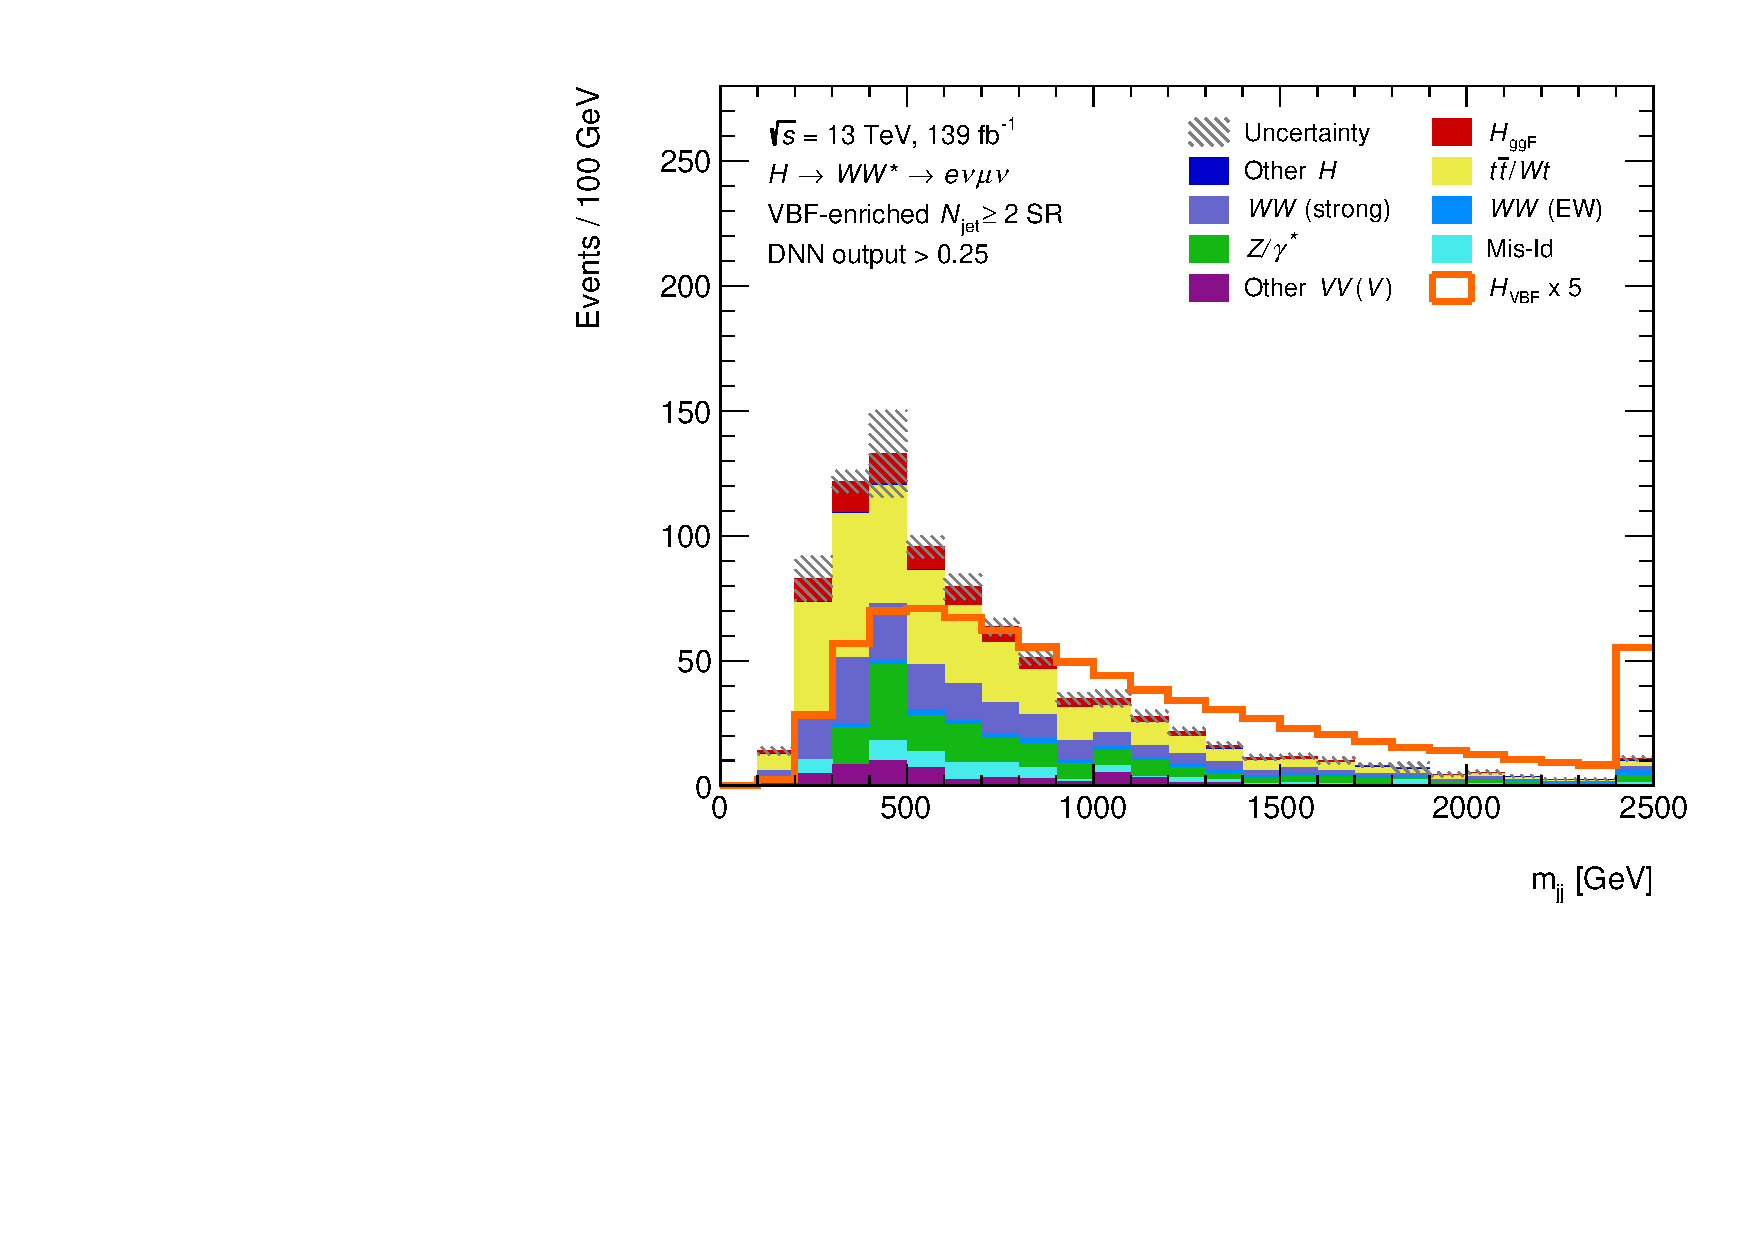
\includegraphics[width=0.32\textwidth]{figures/hww/dnn/blinded/run2-emme-CutVBFSR_DNN25-Mjj-lin.pdf} \hfill
        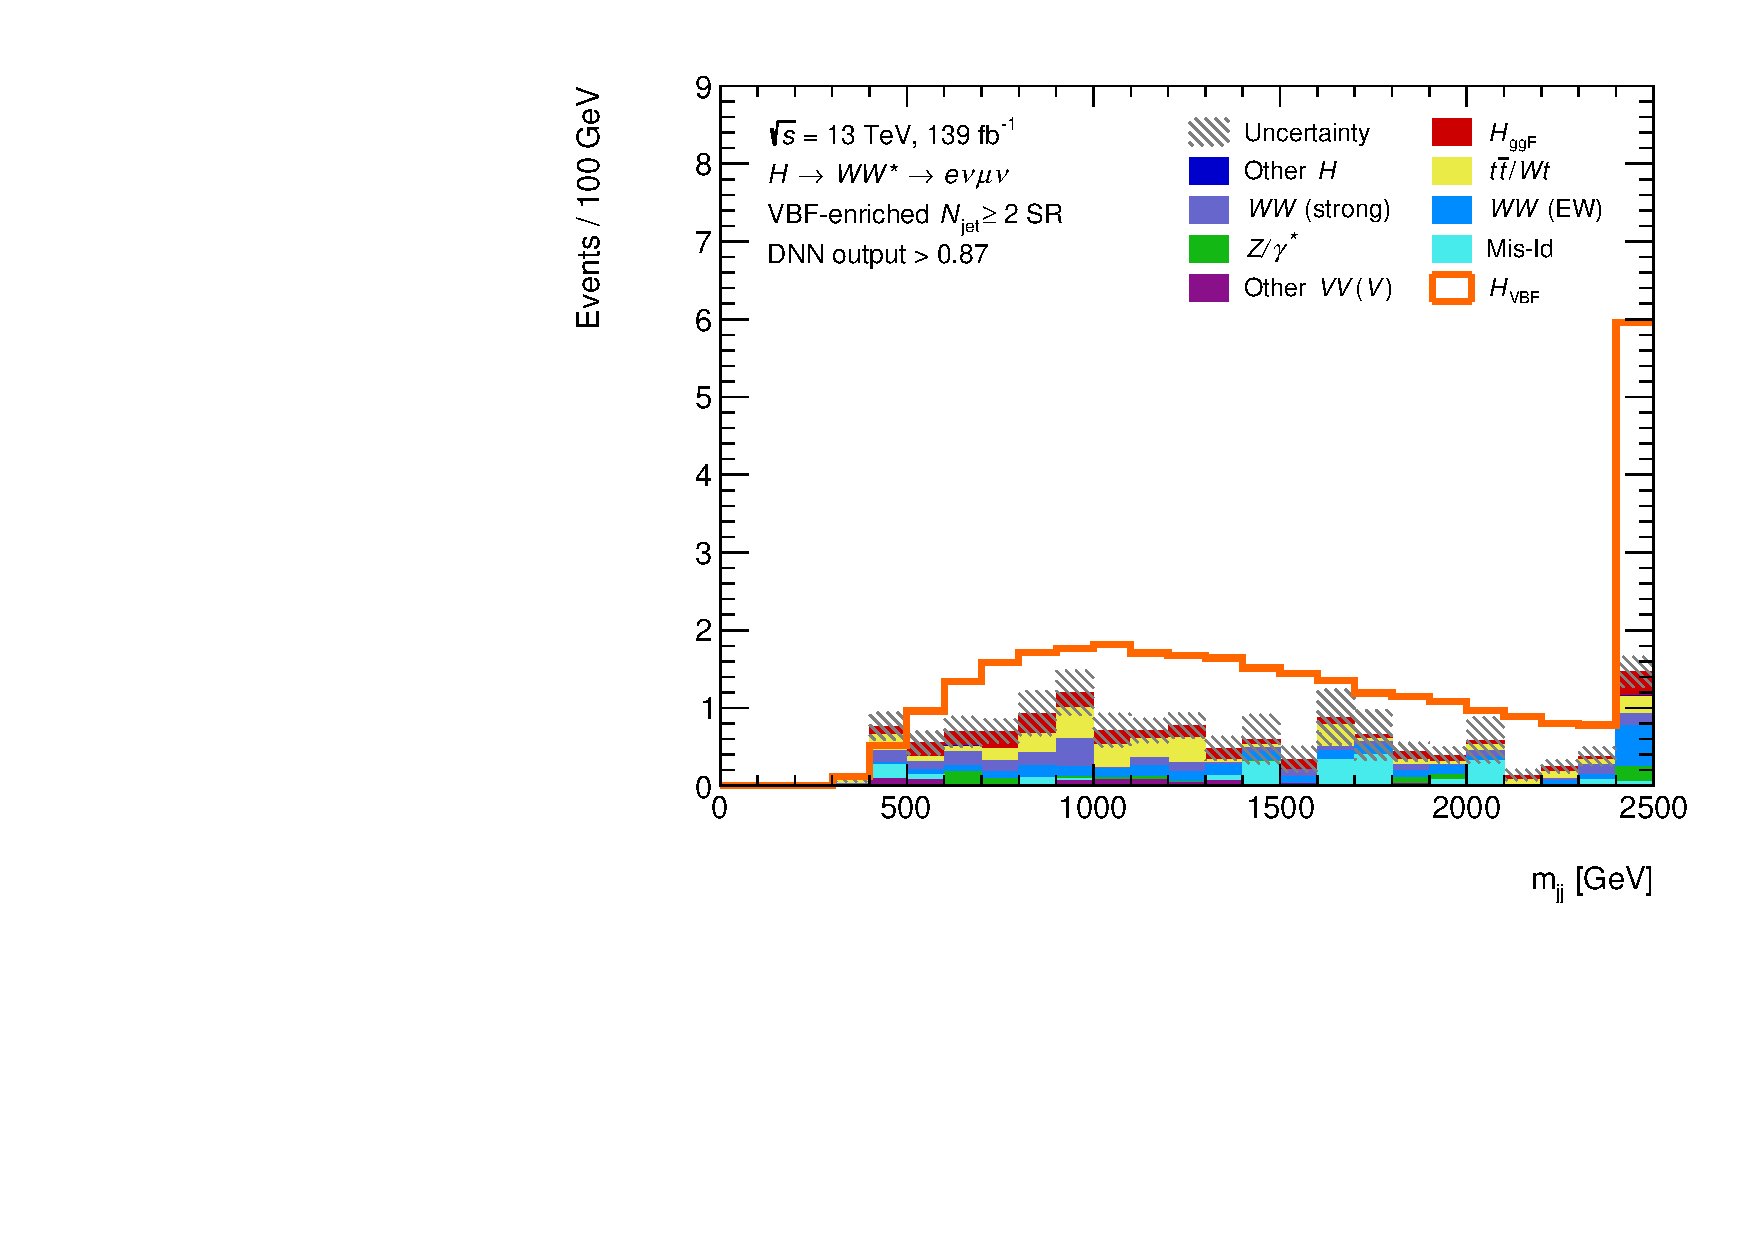
\includegraphics[width=0.32\textwidth]{figures/hww/dnn/blinded/run2-emme-CutVBFSR_DNN87-Mjj-lin.pdf}
    } \\
    \subfloat[$\dyjj$]{
        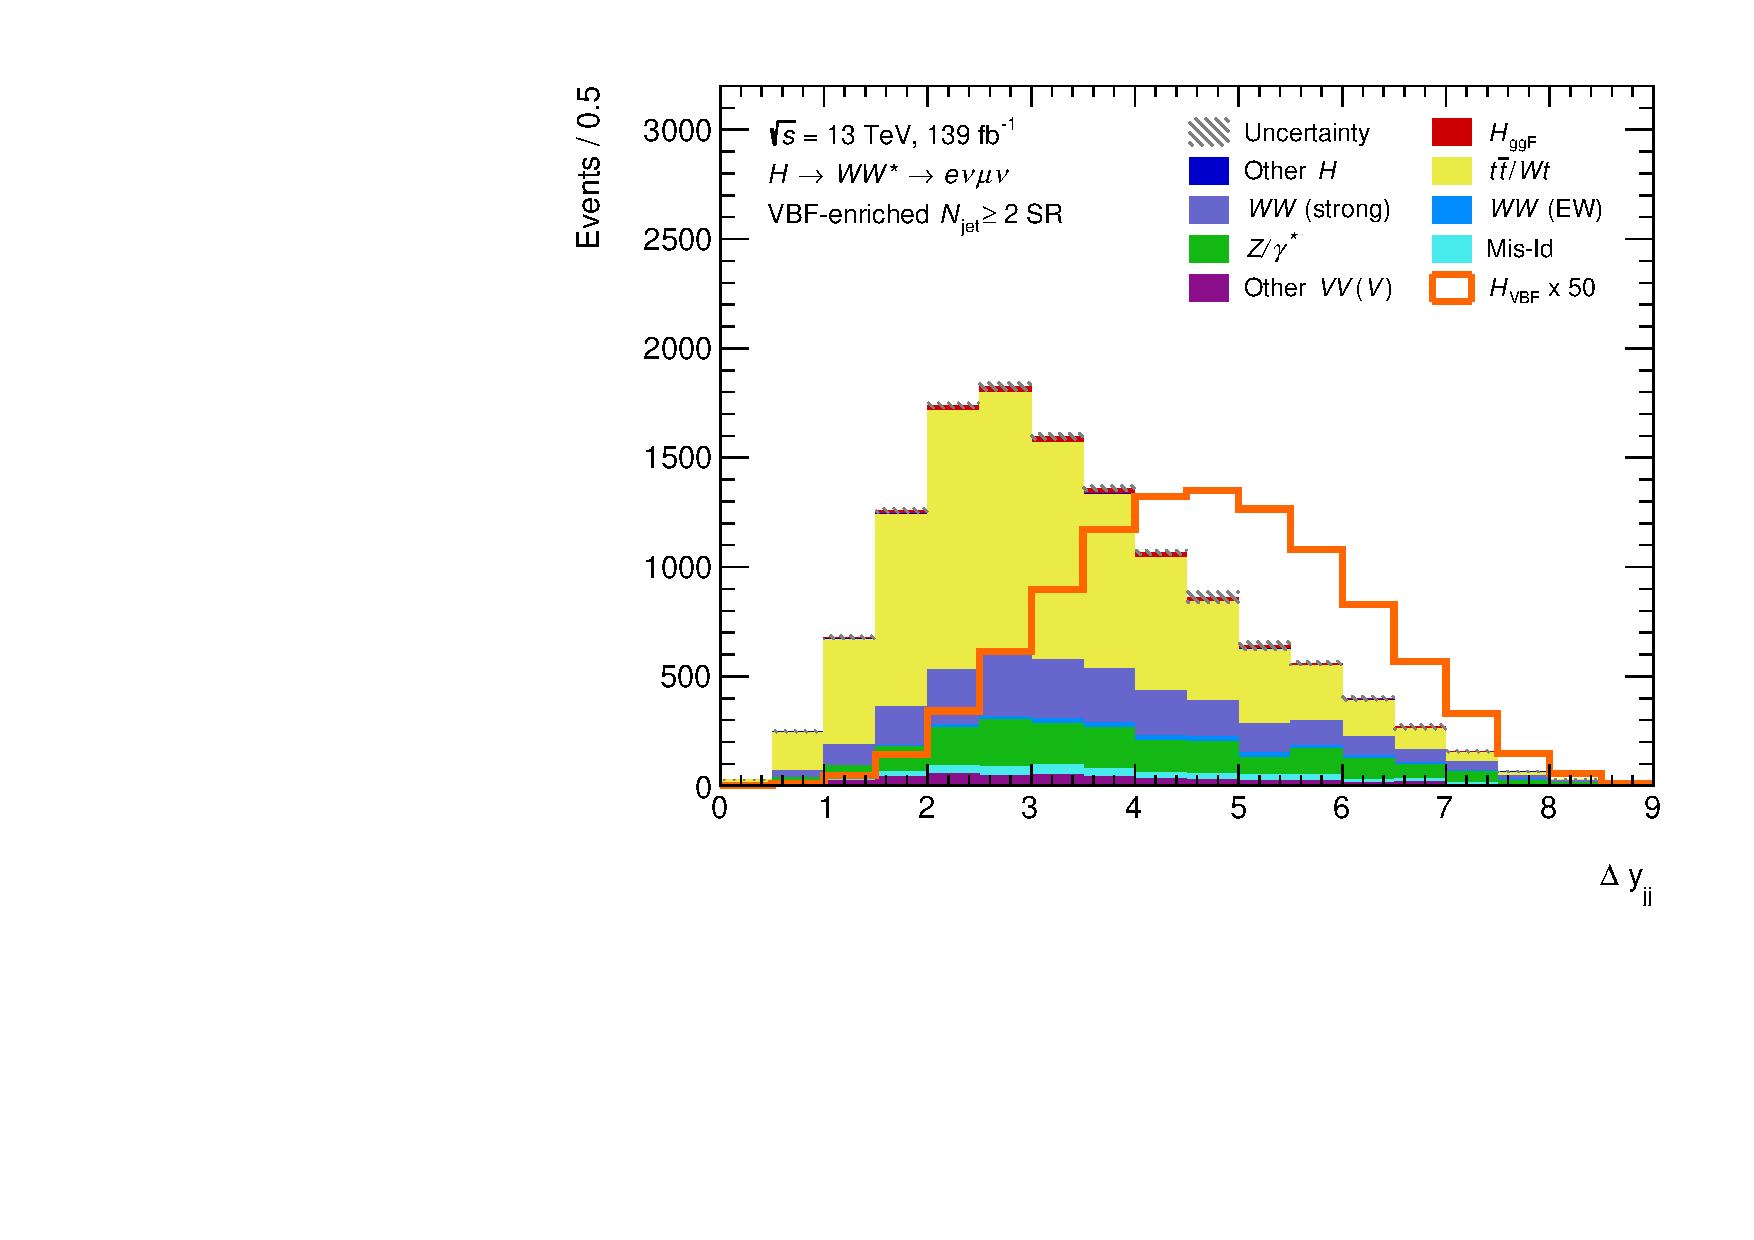
\includegraphics[width=0.32\textwidth]{figures/hww/dnn/blinded/run2-emme-CutVBF_SR-DYjj-lin.pdf} \hfill
        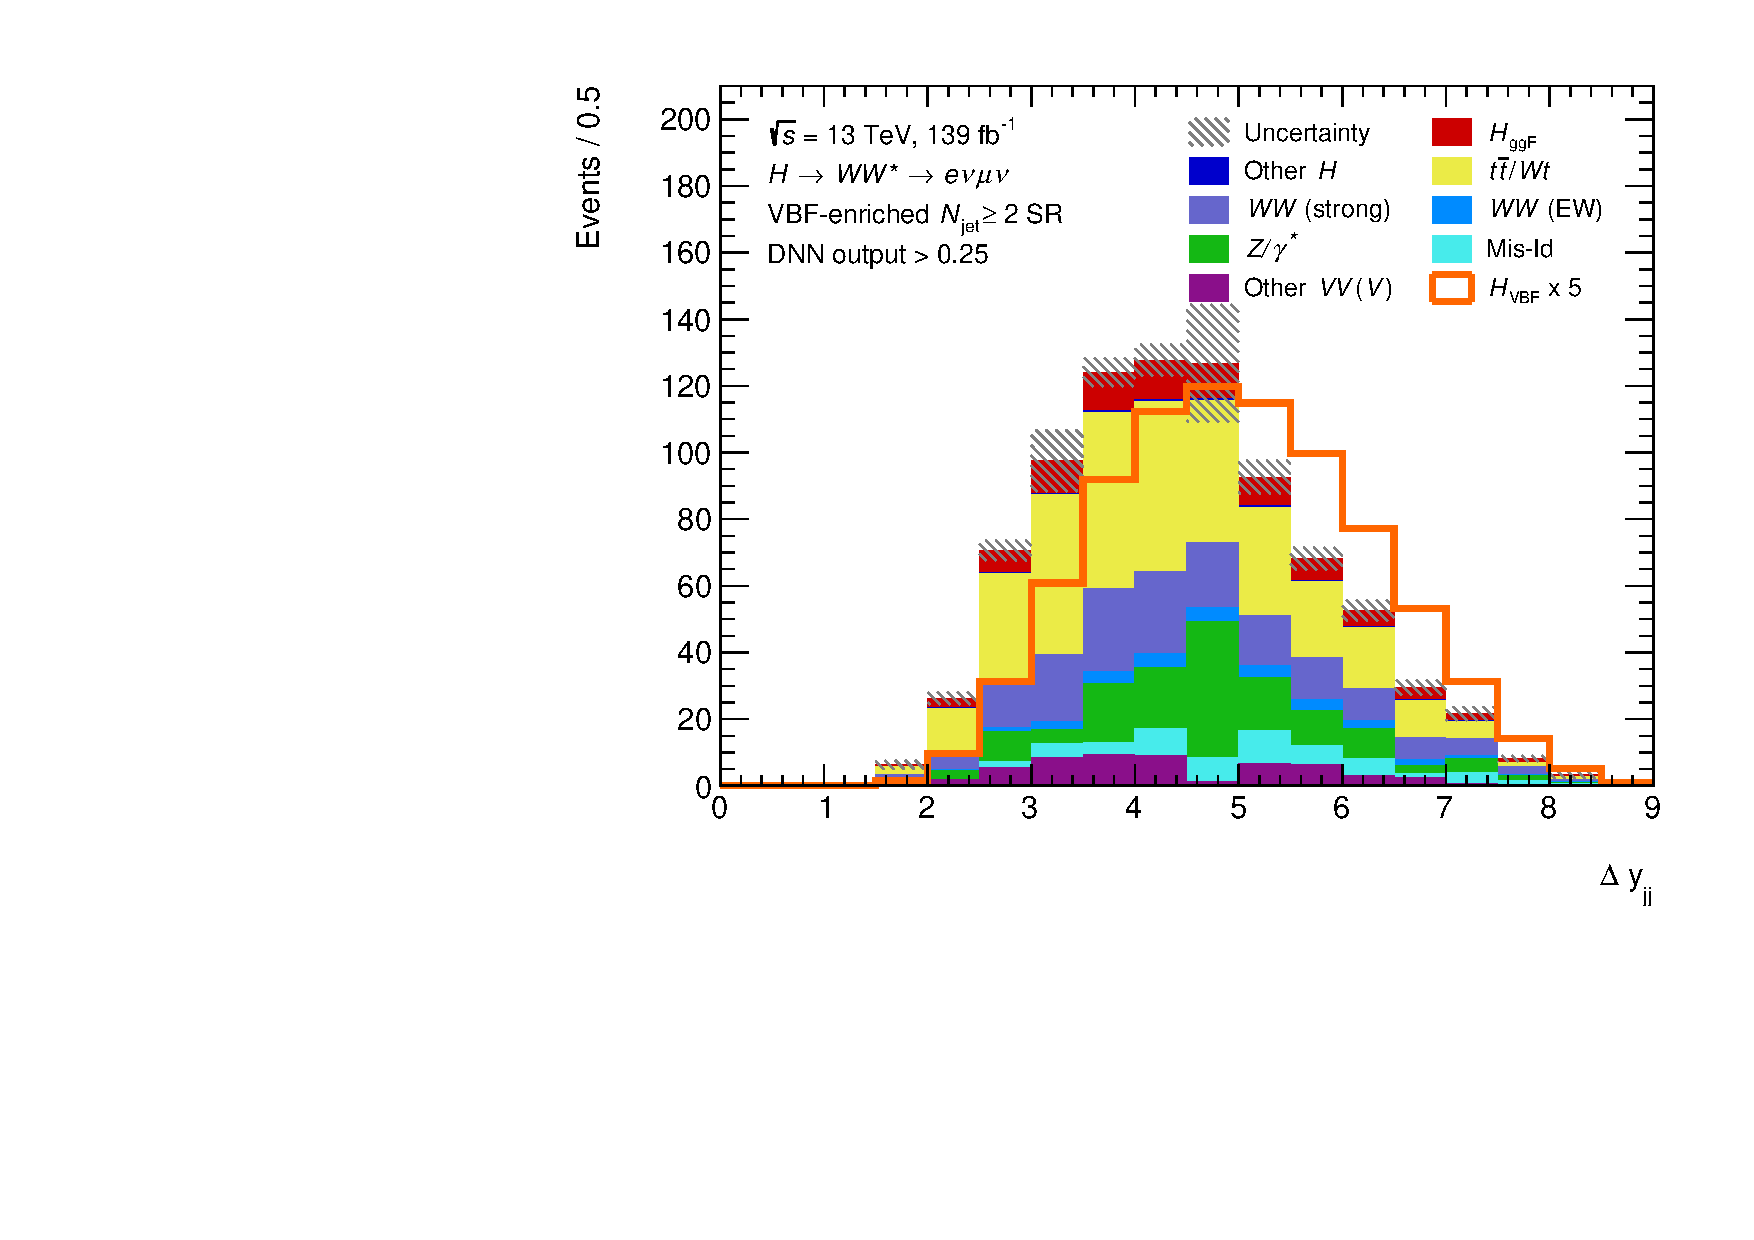
\includegraphics[width=0.32\textwidth]{figures/hww/dnn/blinded/run2-emme-CutVBFSR_DNN25-DYjj-lin.pdf} \hfill
        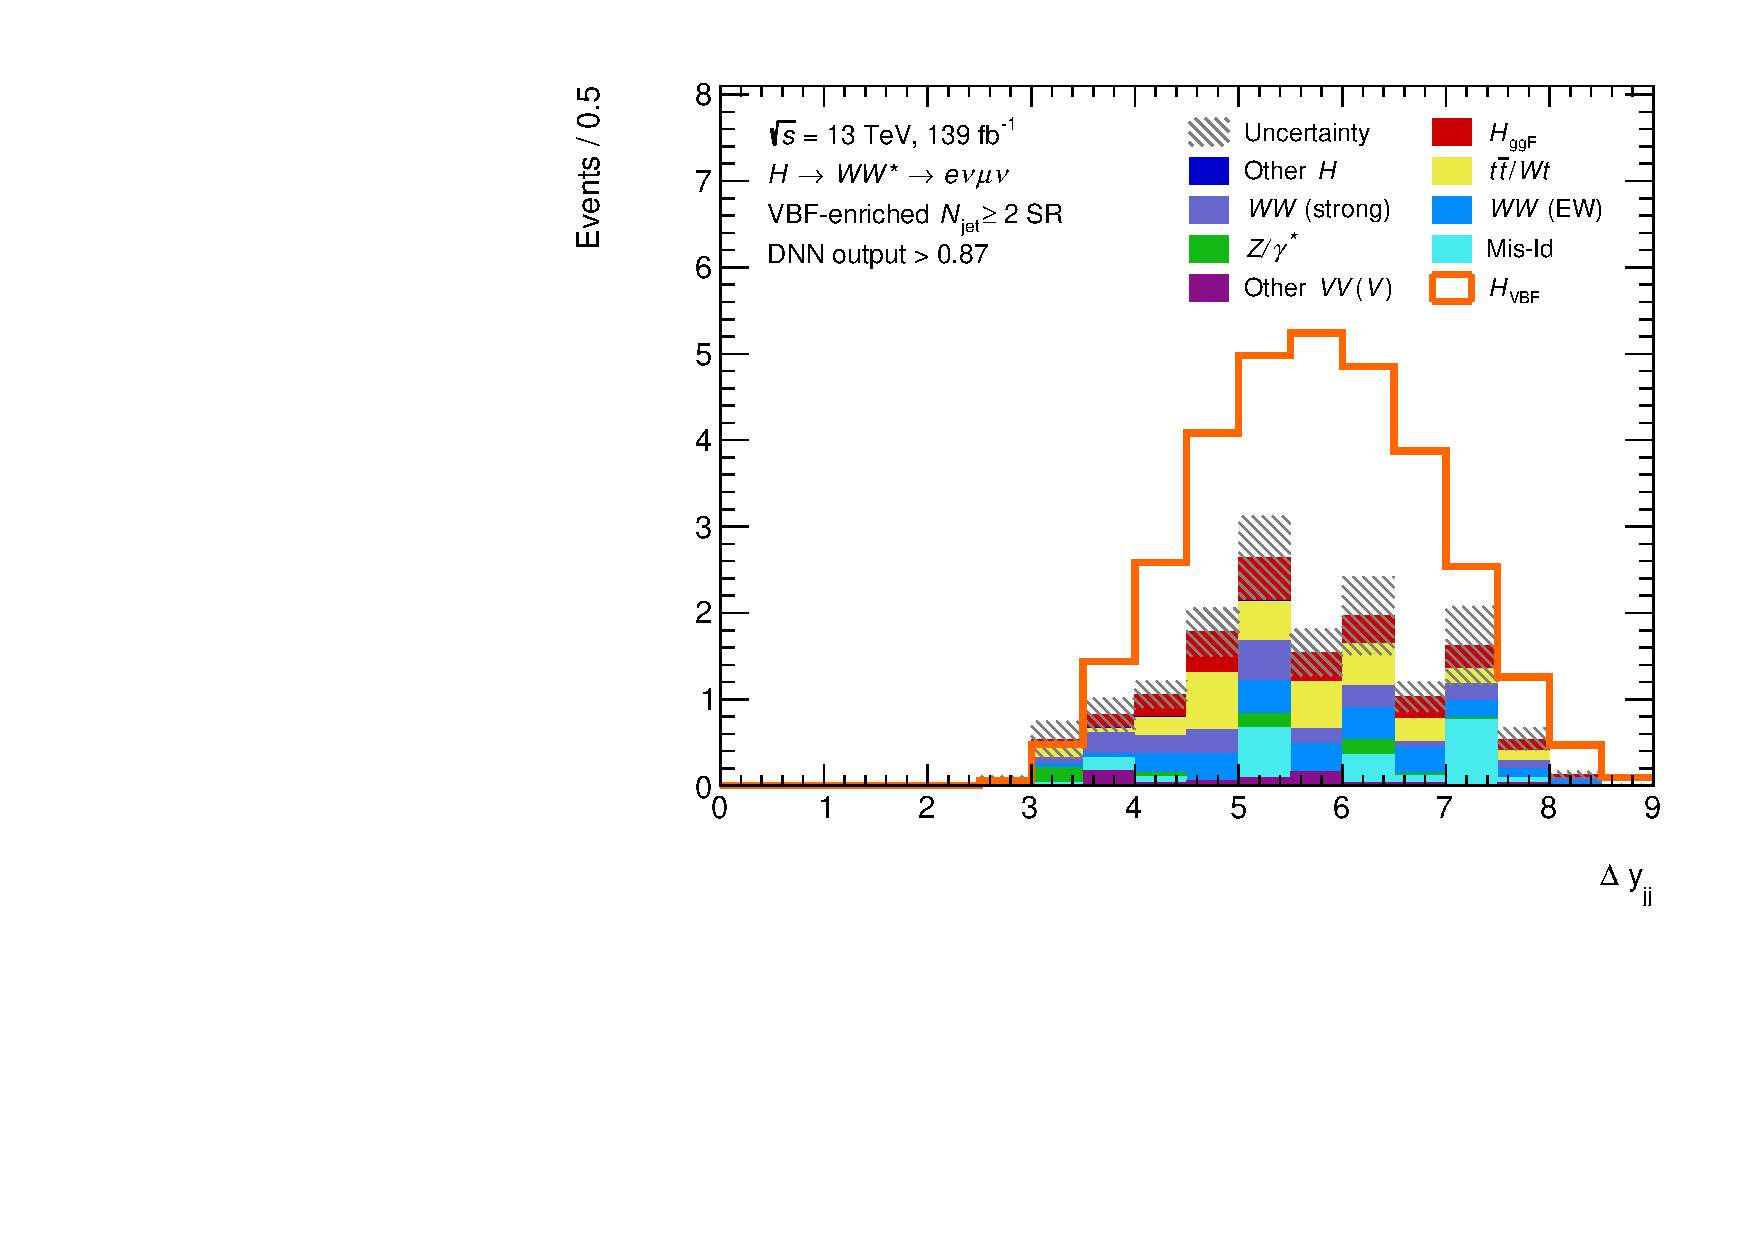
\includegraphics[width=0.32\textwidth]{figures/hww/dnn/blinded/run2-emme-CutVBFSR_DNN87-DYjj-lin.pdf}
    } \\
    \subfloat[$\lepetacent$]{
        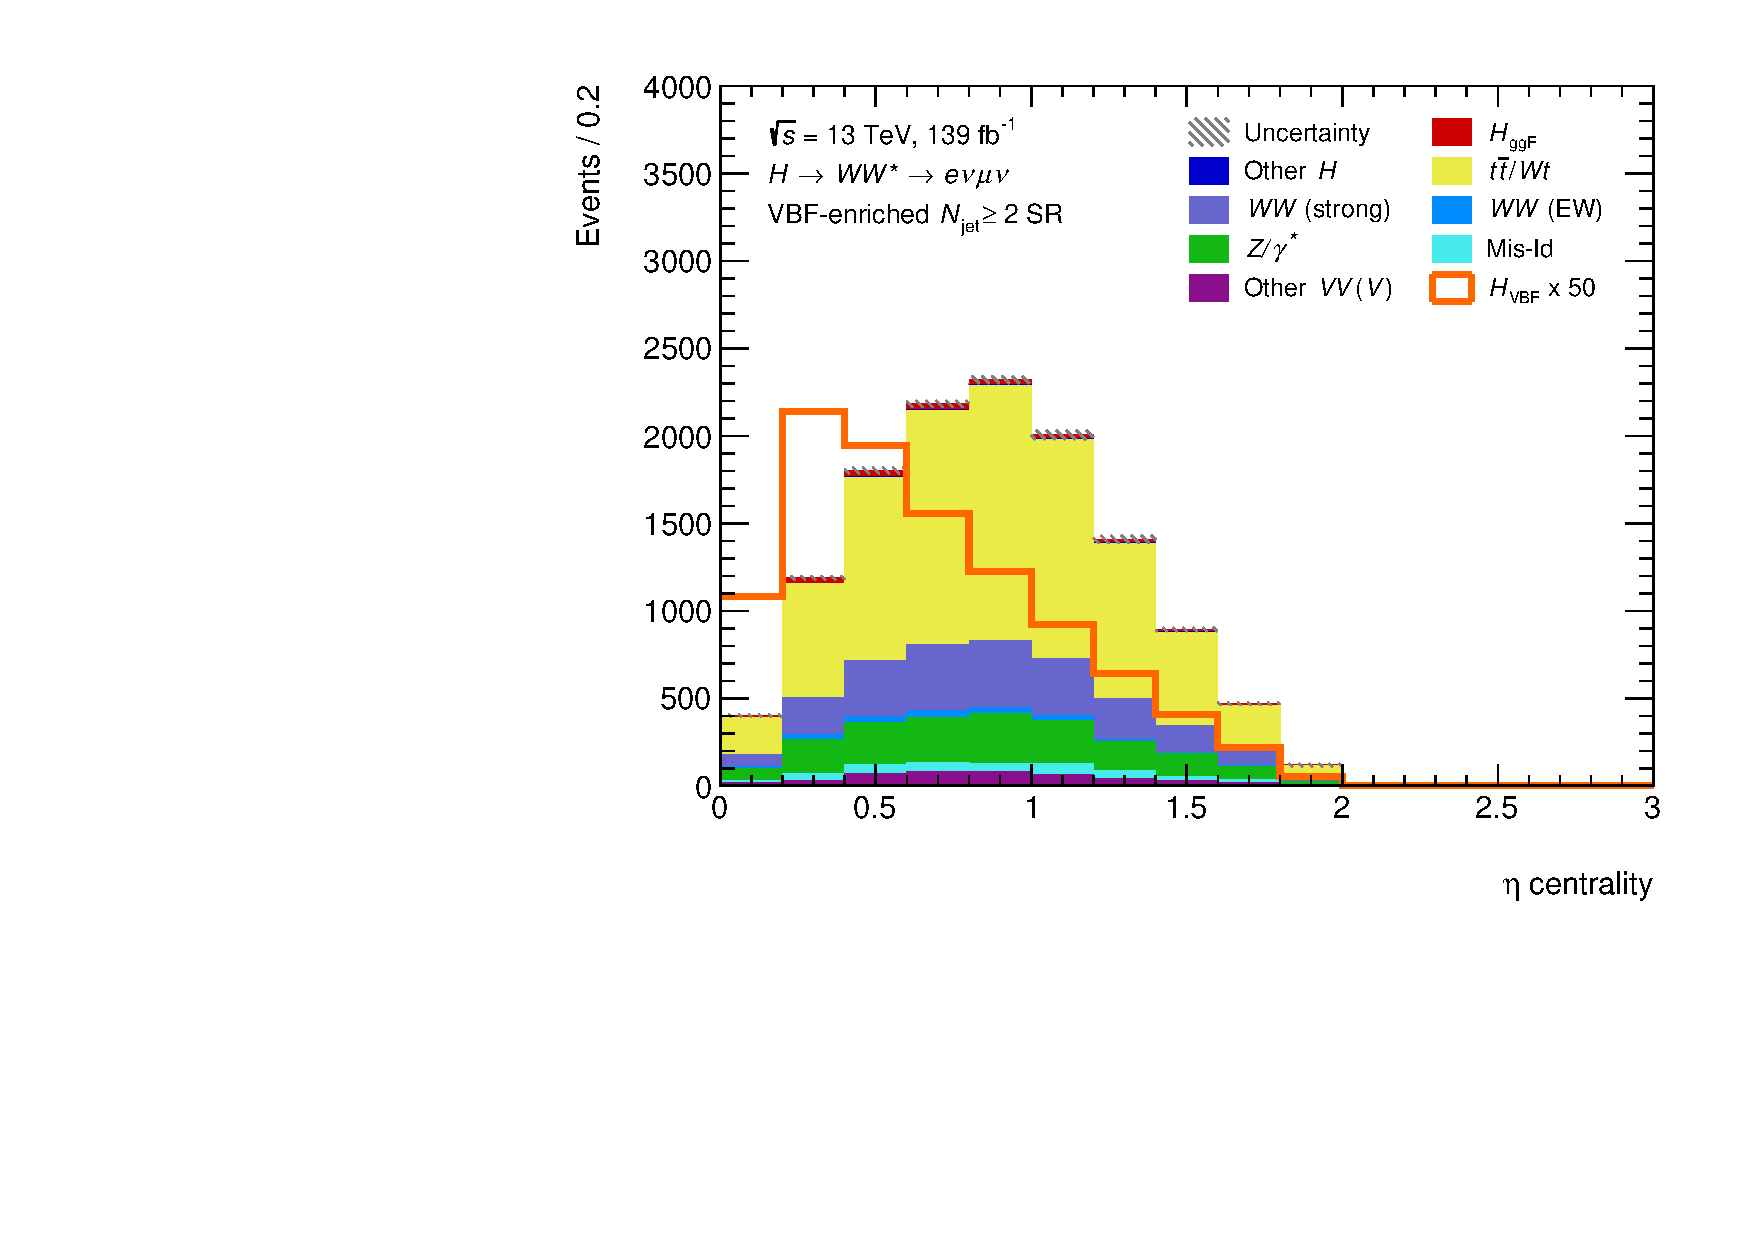
\includegraphics[width=0.32\textwidth]{figures/hww/dnn/blinded/run2-emme-CutVBF_SR-contOLV-lin.pdf} \hfill
        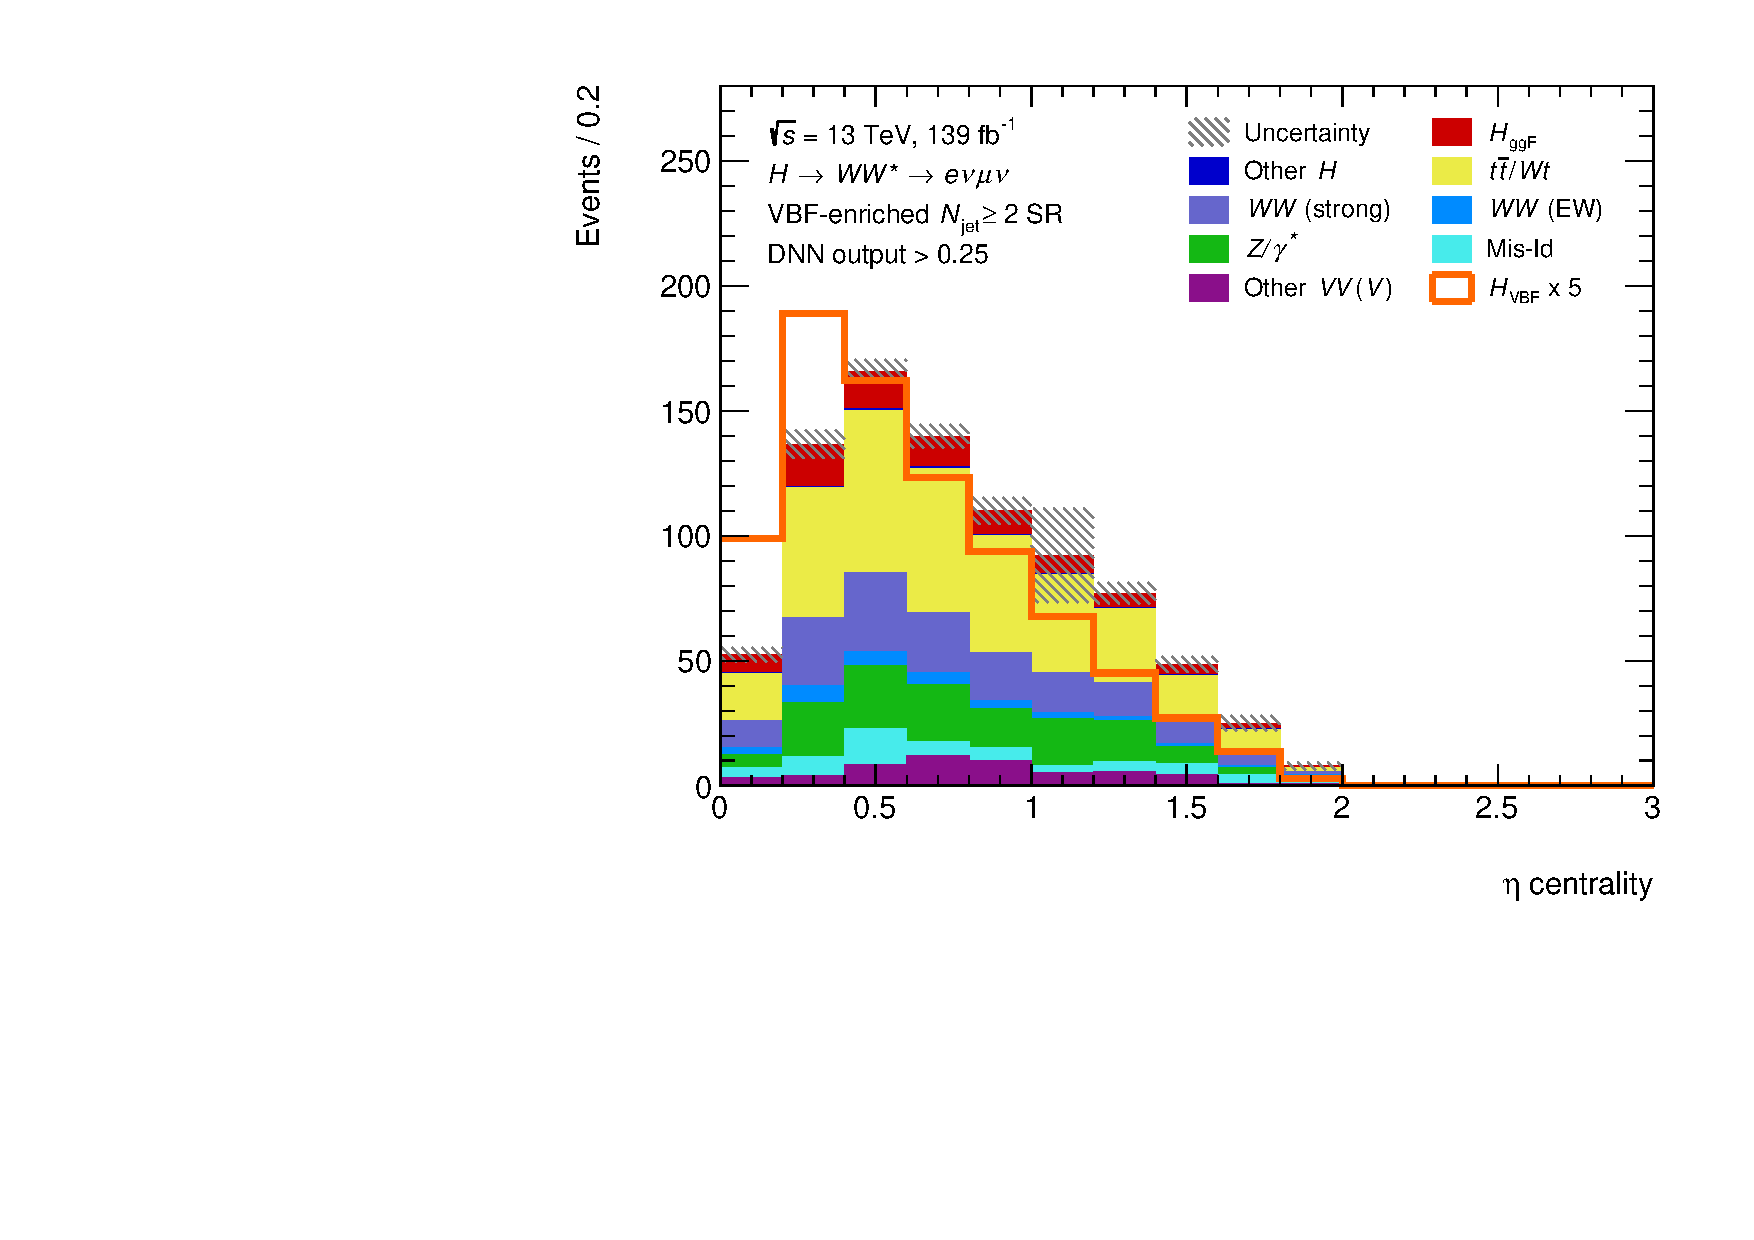
\includegraphics[width=0.32\textwidth]{figures/hww/dnn/blinded/run2-emme-CutVBFSR_DNN25-contOLV-lin.pdf} \hfill
        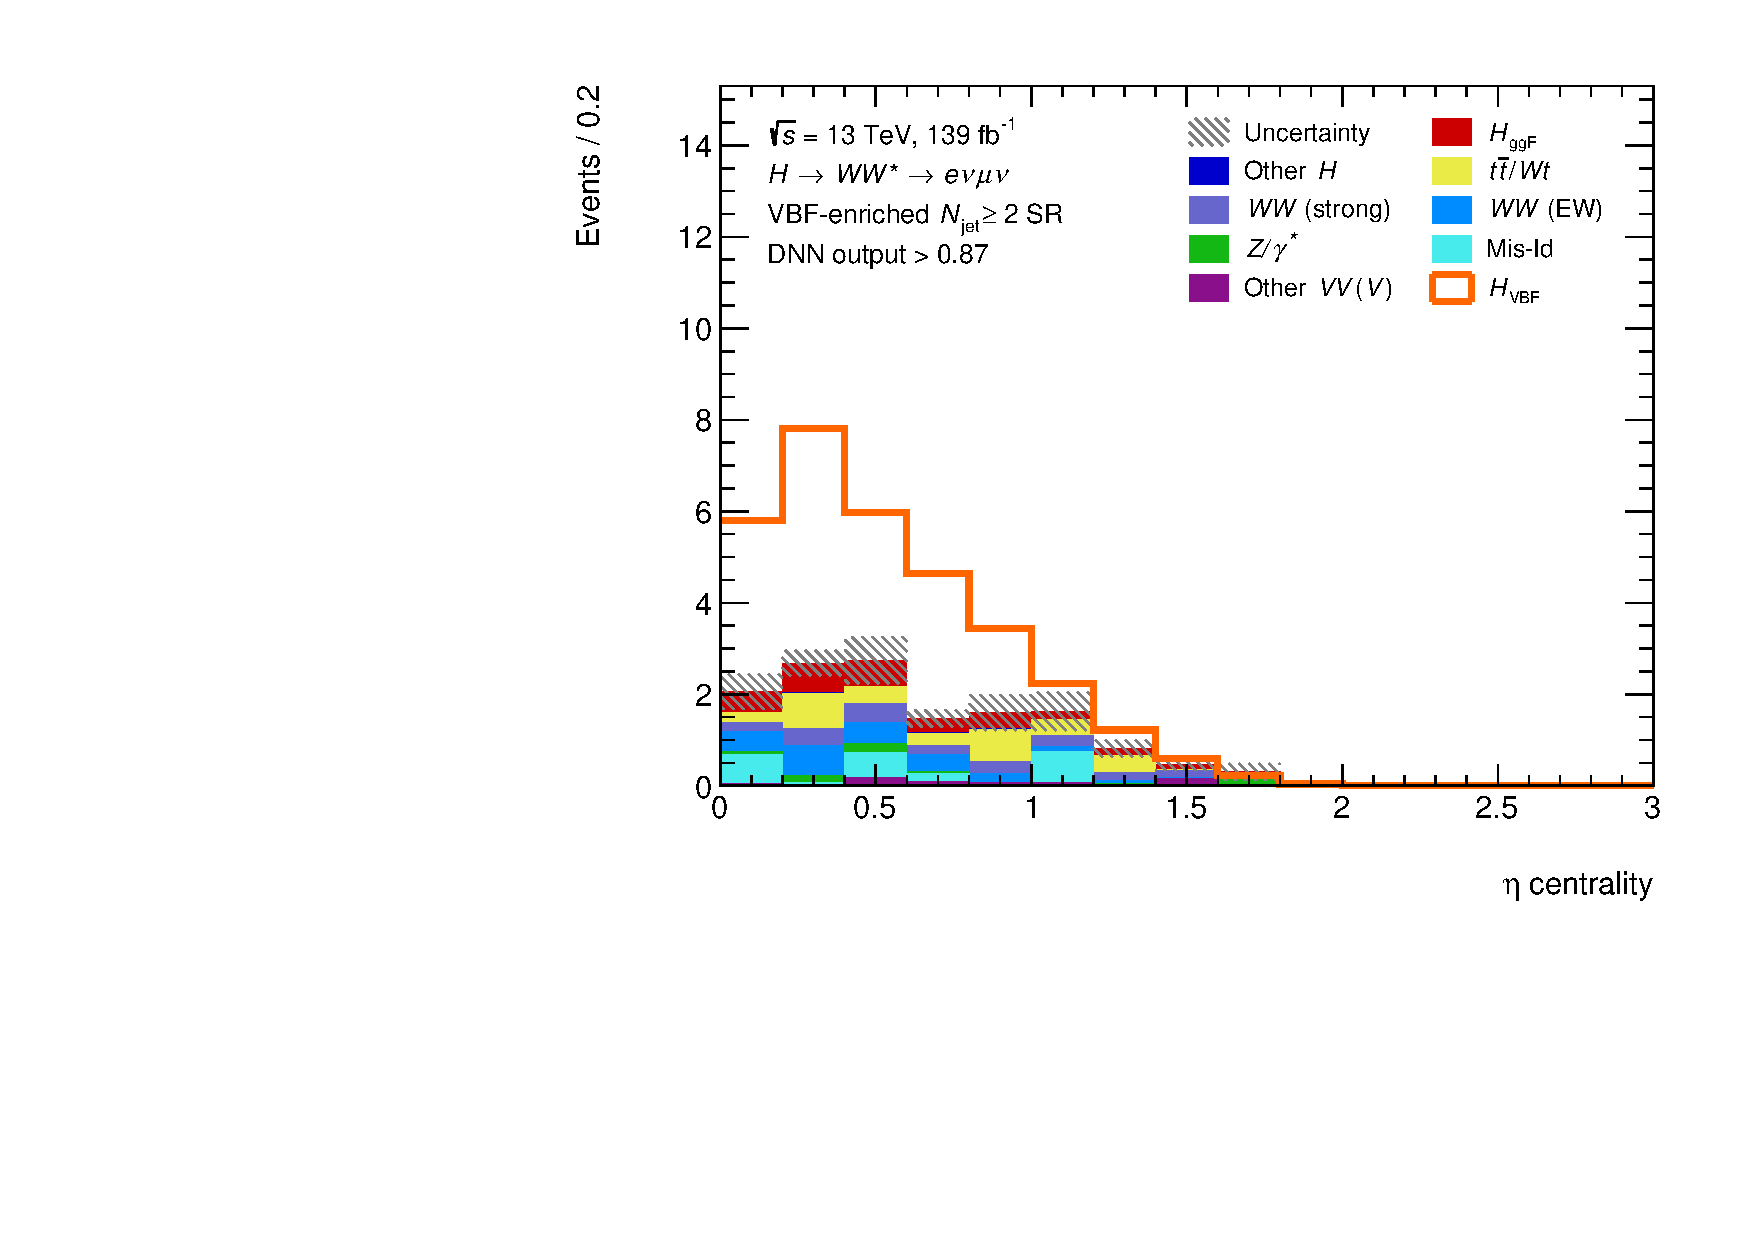
\includegraphics[width=0.32\textwidth]{figures/hww/dnn/blinded/run2-emme-CutVBFSR_DNN87-contOLV-lin.pdf}
    } \\
    {\caption{Distributions of $\dphill$, $\mll$, $\lepetacent$ in the VBF signal region.
        Each row corresponds to one variable with different selections made on the DNN output.
        \label{app:fig:dnn-inputs-vbf-top1} }}
\end{figure}


\begin{figure}[h]
    \centering
    \subfloat[$\mlonejtwo$]{
        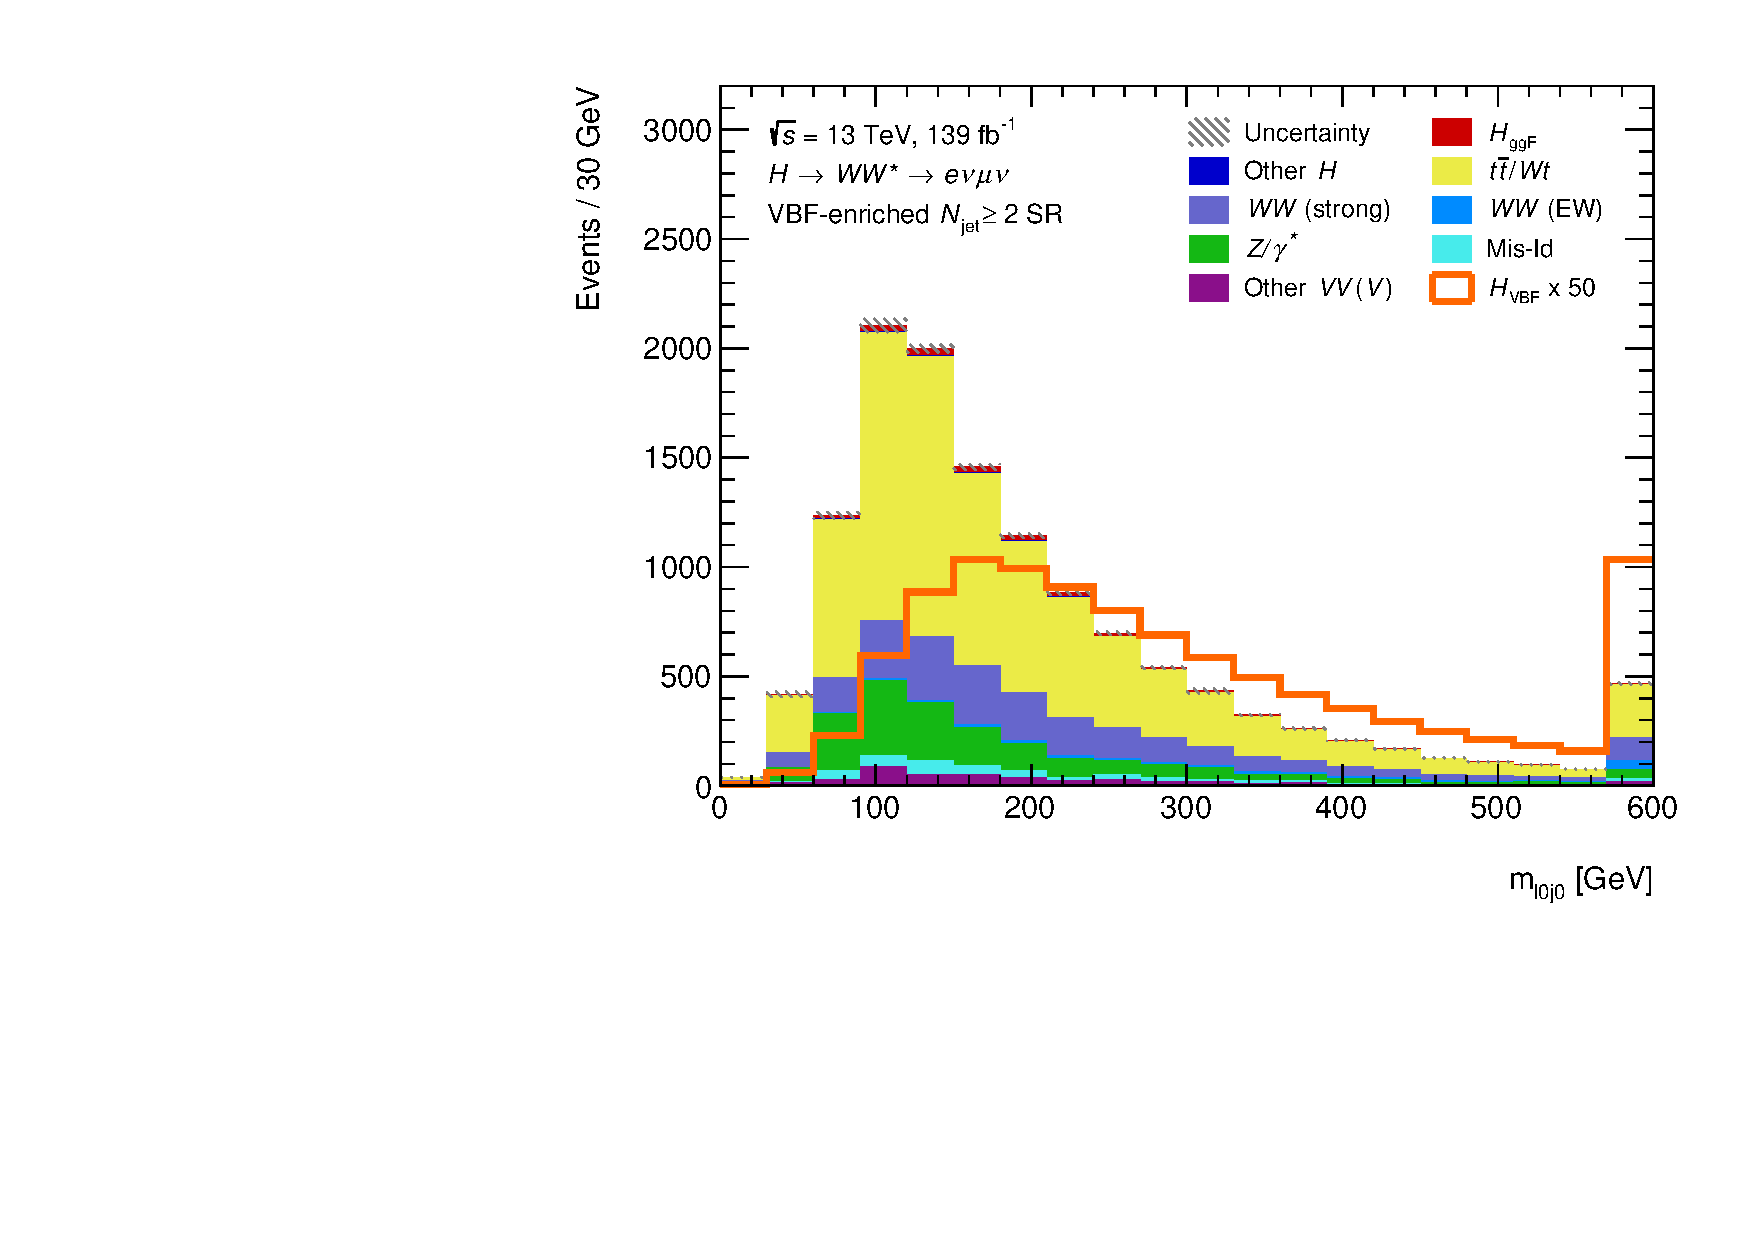
\includegraphics[width=0.32\textwidth]{figures/hww/dnn/blinded/run2-emme-CutVBF_SR-Ml0j0-lin.pdf} \hfill
        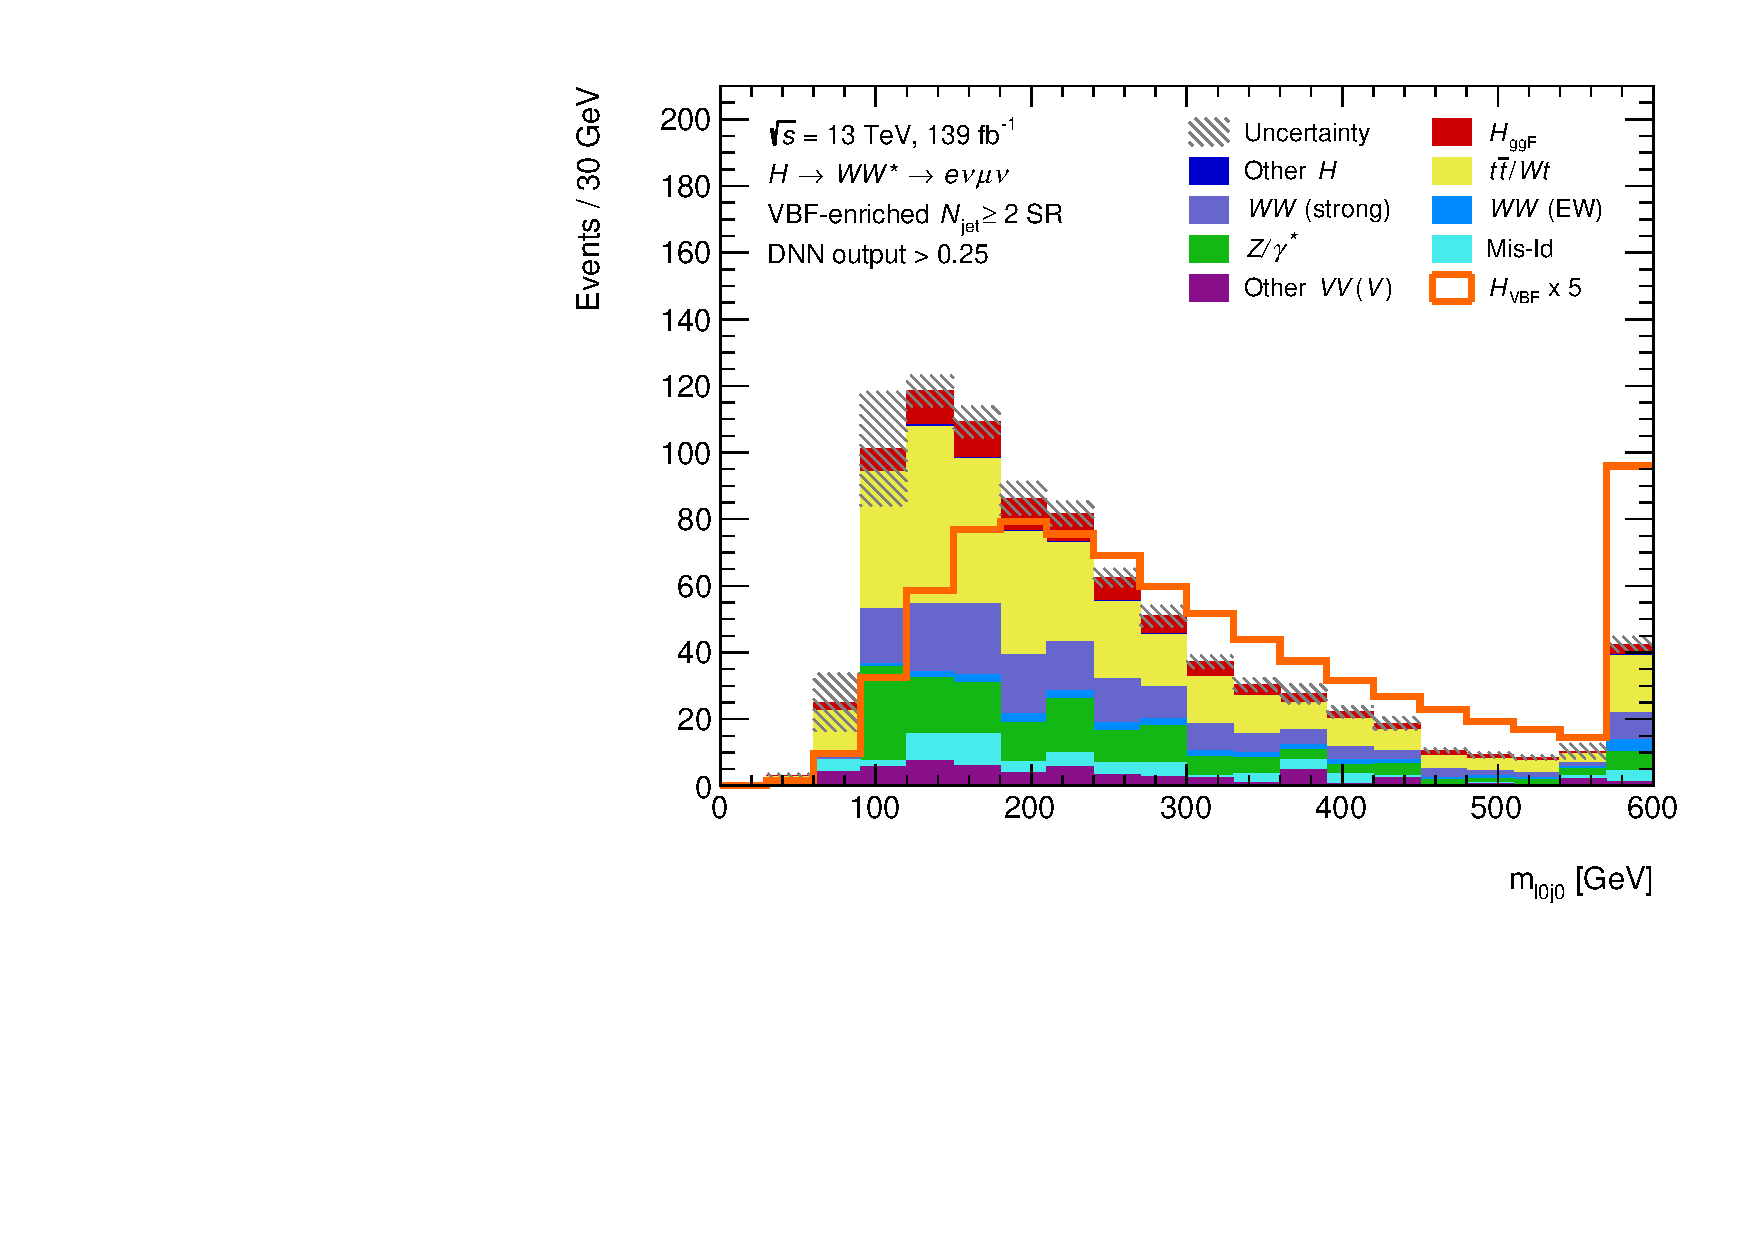
\includegraphics[width=0.32\textwidth]{figures/hww/dnn/blinded/run2-emme-CutVBFSR_DNN25-Ml0j0-lin.pdf} \hfill
        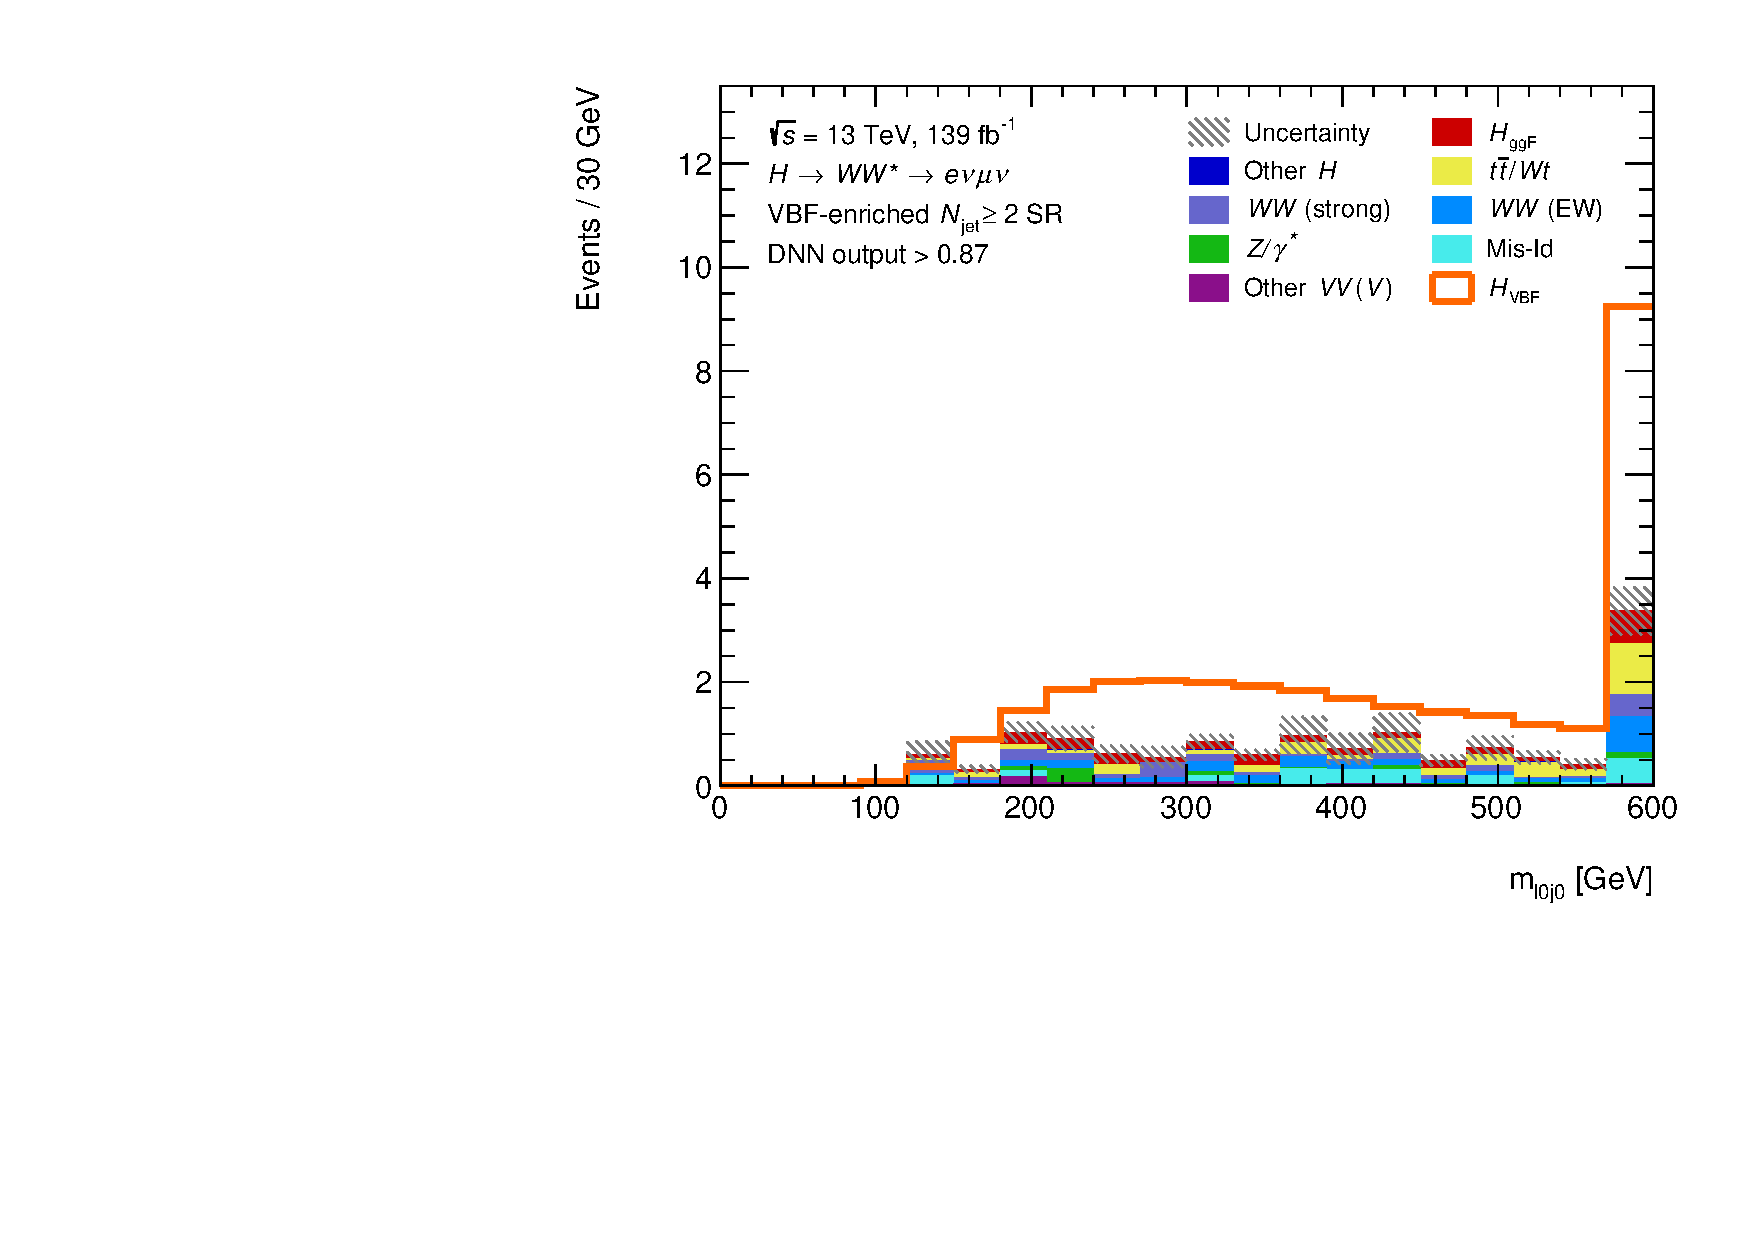
\includegraphics[width=0.32\textwidth]{figures/hww/dnn/blinded/run2-emme-CutVBFSR_DNN87-Ml0j0-lin.pdf}
    } \\
    \subfloat[$\mltwojone$]{
        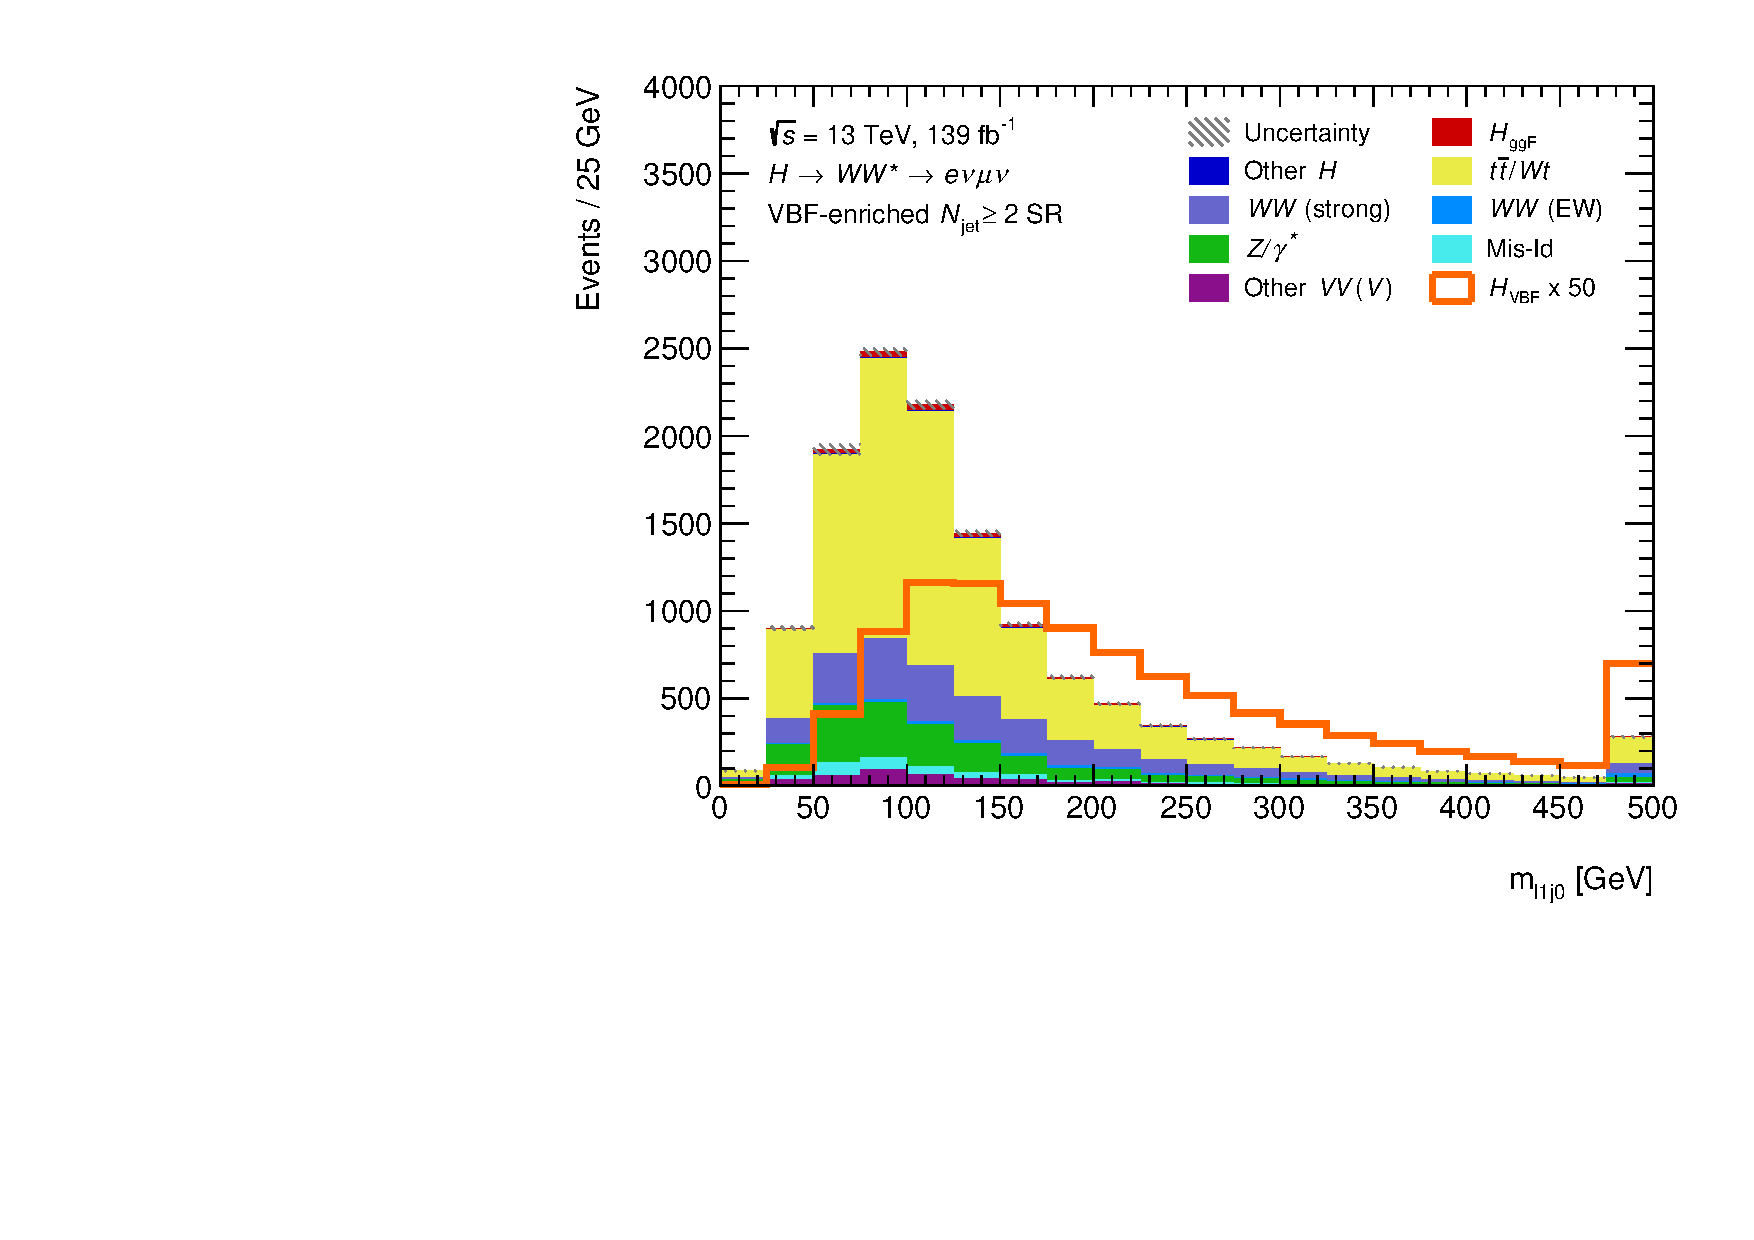
\includegraphics[width=0.32\textwidth]{figures/hww/dnn/blinded/run2-emme-CutVBF_SR-Ml1j0-lin.pdf} \hfill
        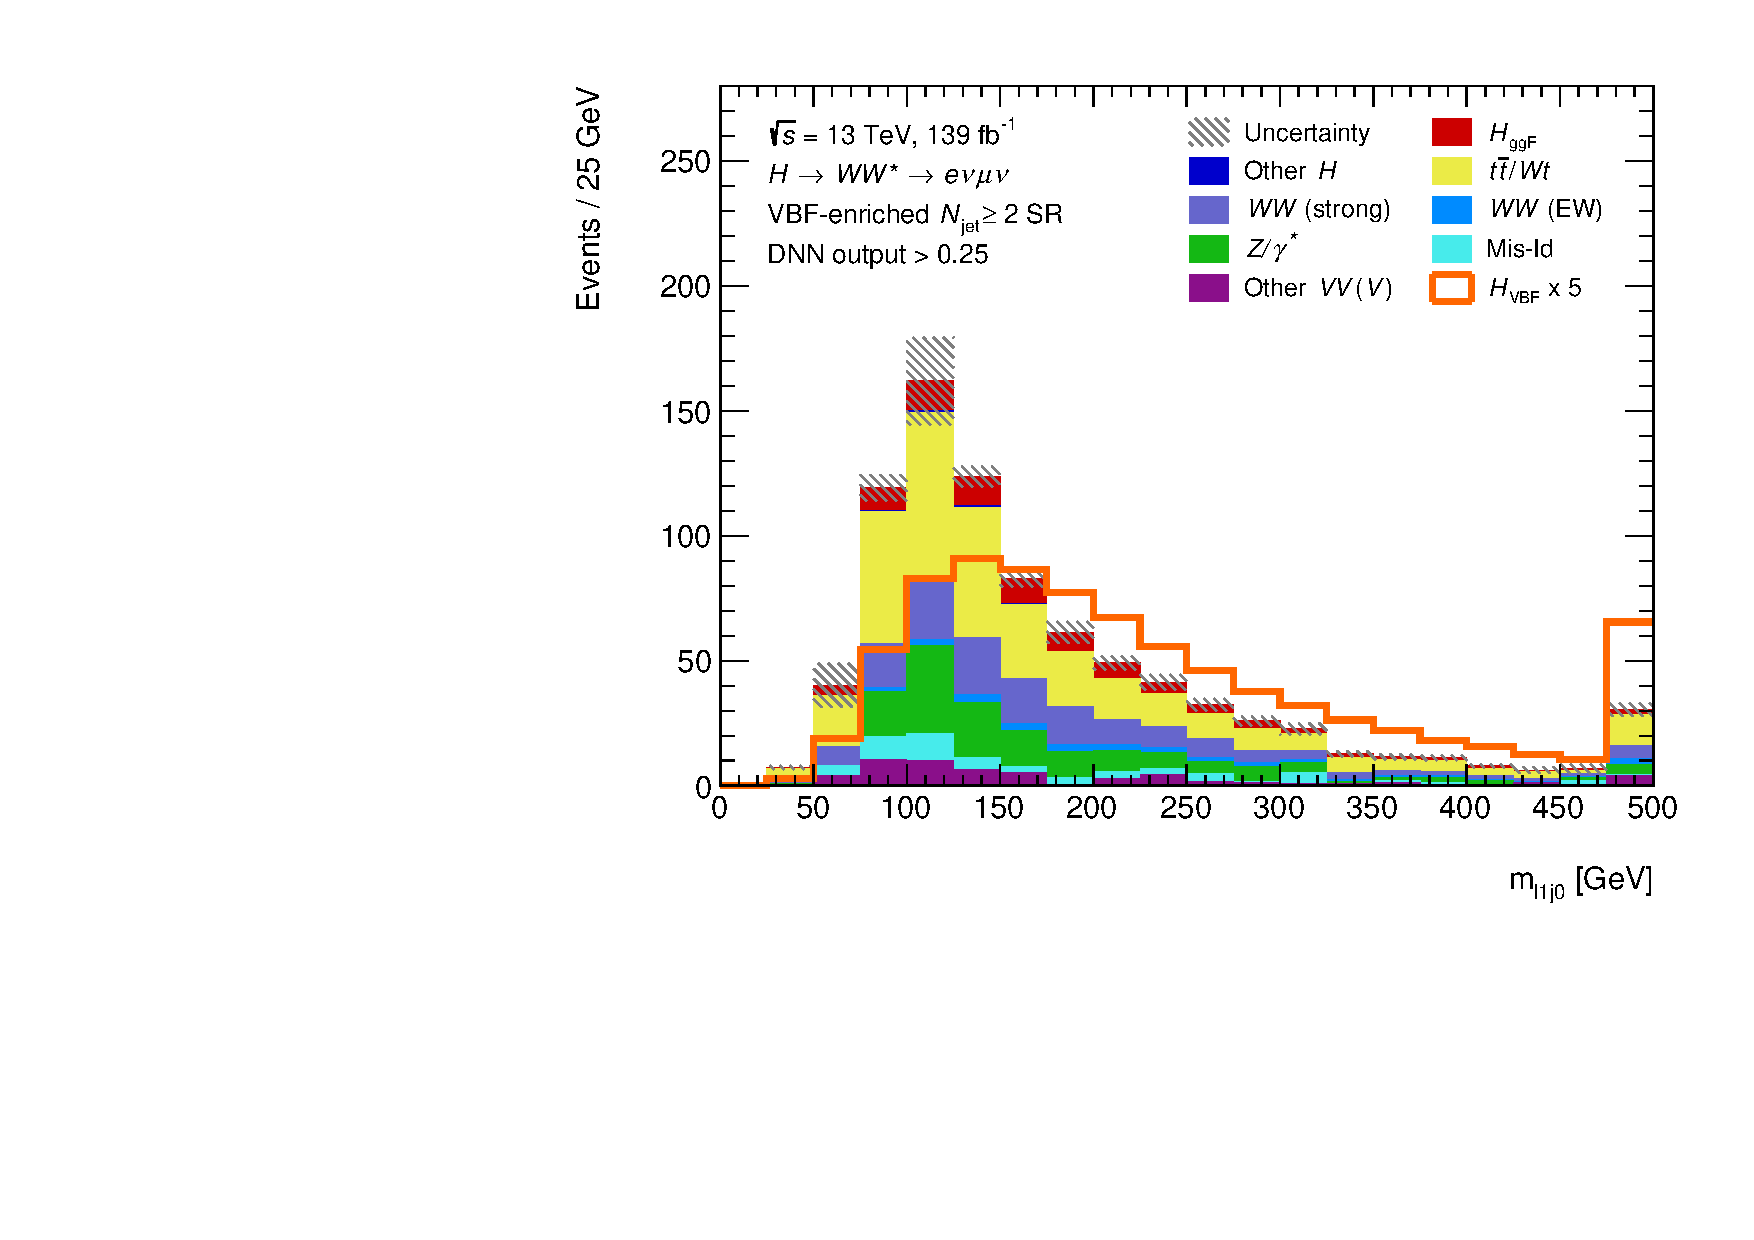
\includegraphics[width=0.32\textwidth]{figures/hww/dnn/blinded/run2-emme-CutVBFSR_DNN25-Ml1j0-lin.pdf} \hfill
        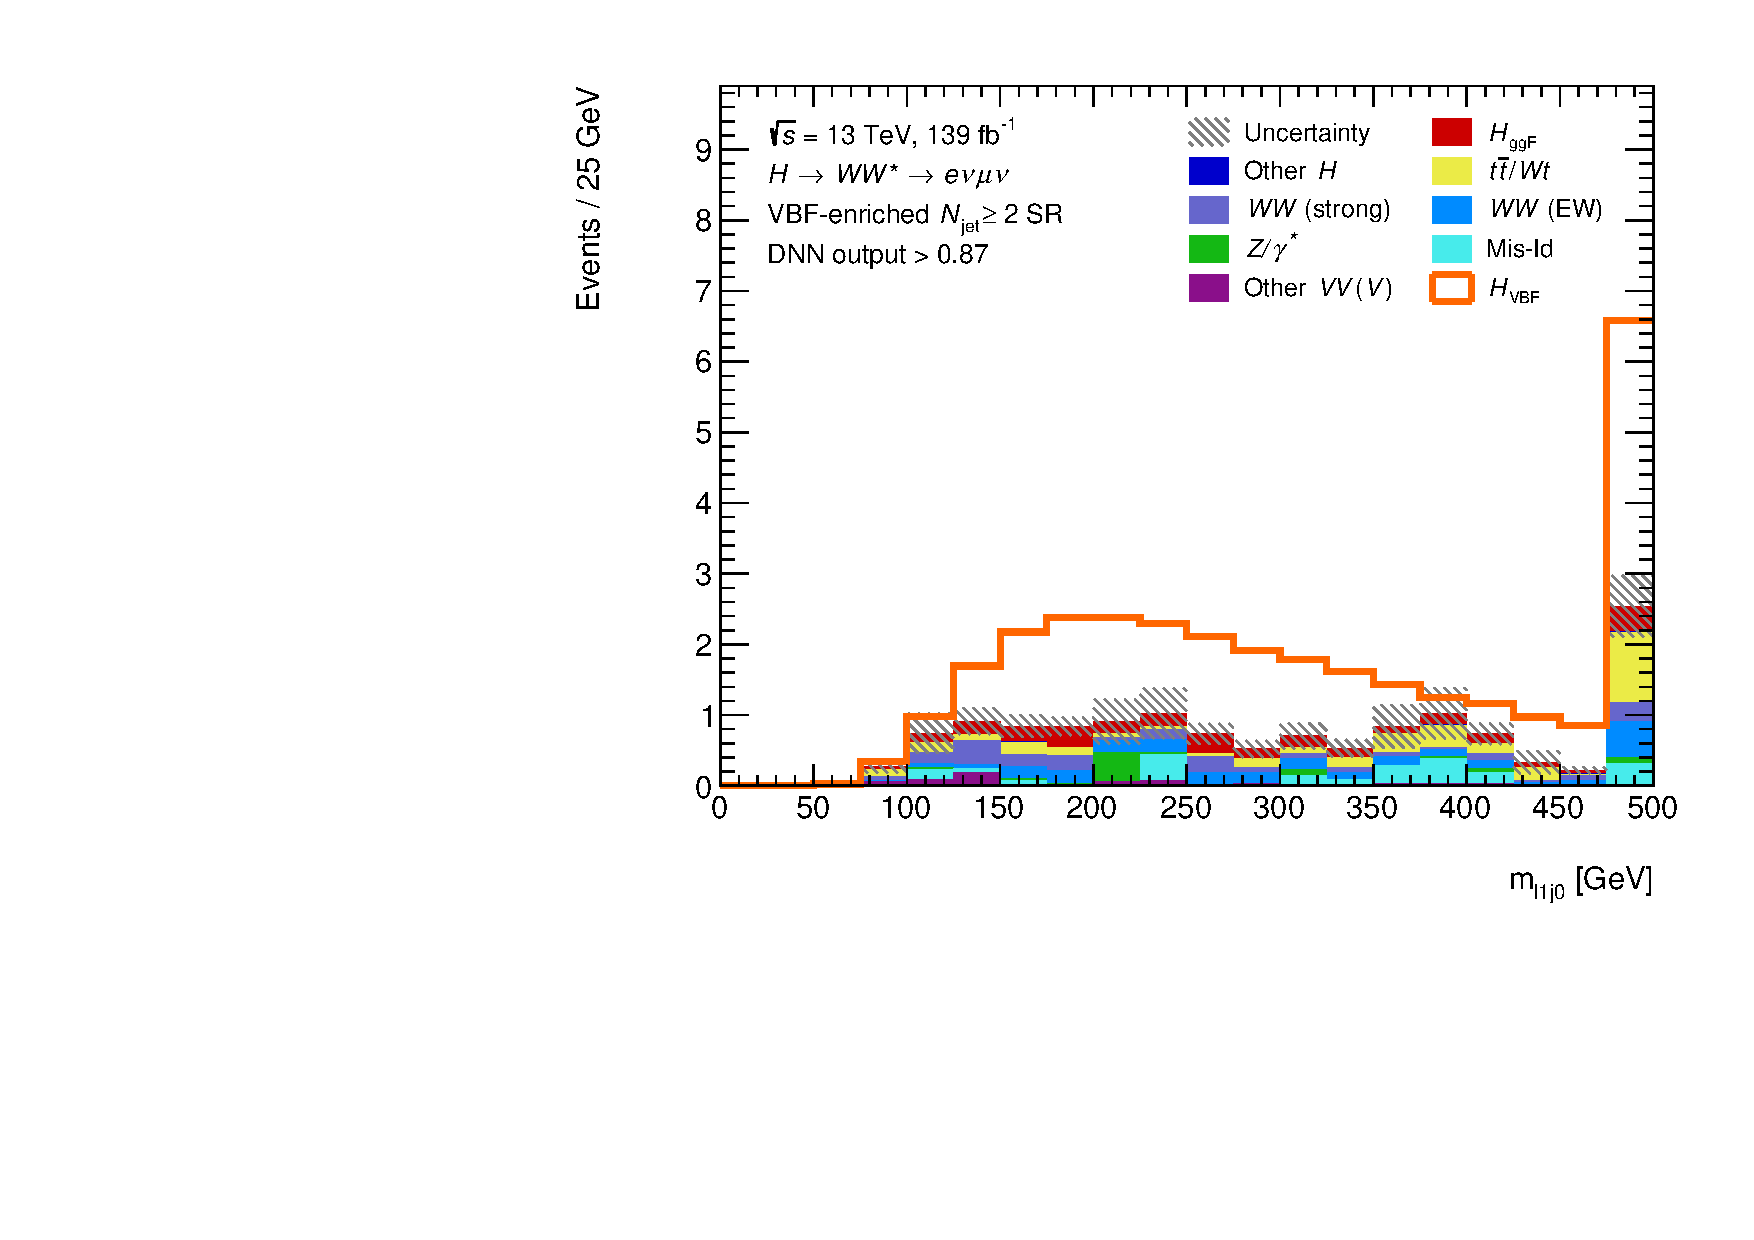
\includegraphics[width=0.32\textwidth]{figures/hww/dnn/blinded/run2-emme-CutVBFSR_DNN87-Ml1j0-lin.pdf}
    } \\
    \subfloat[$\mlonejtwo$]{
        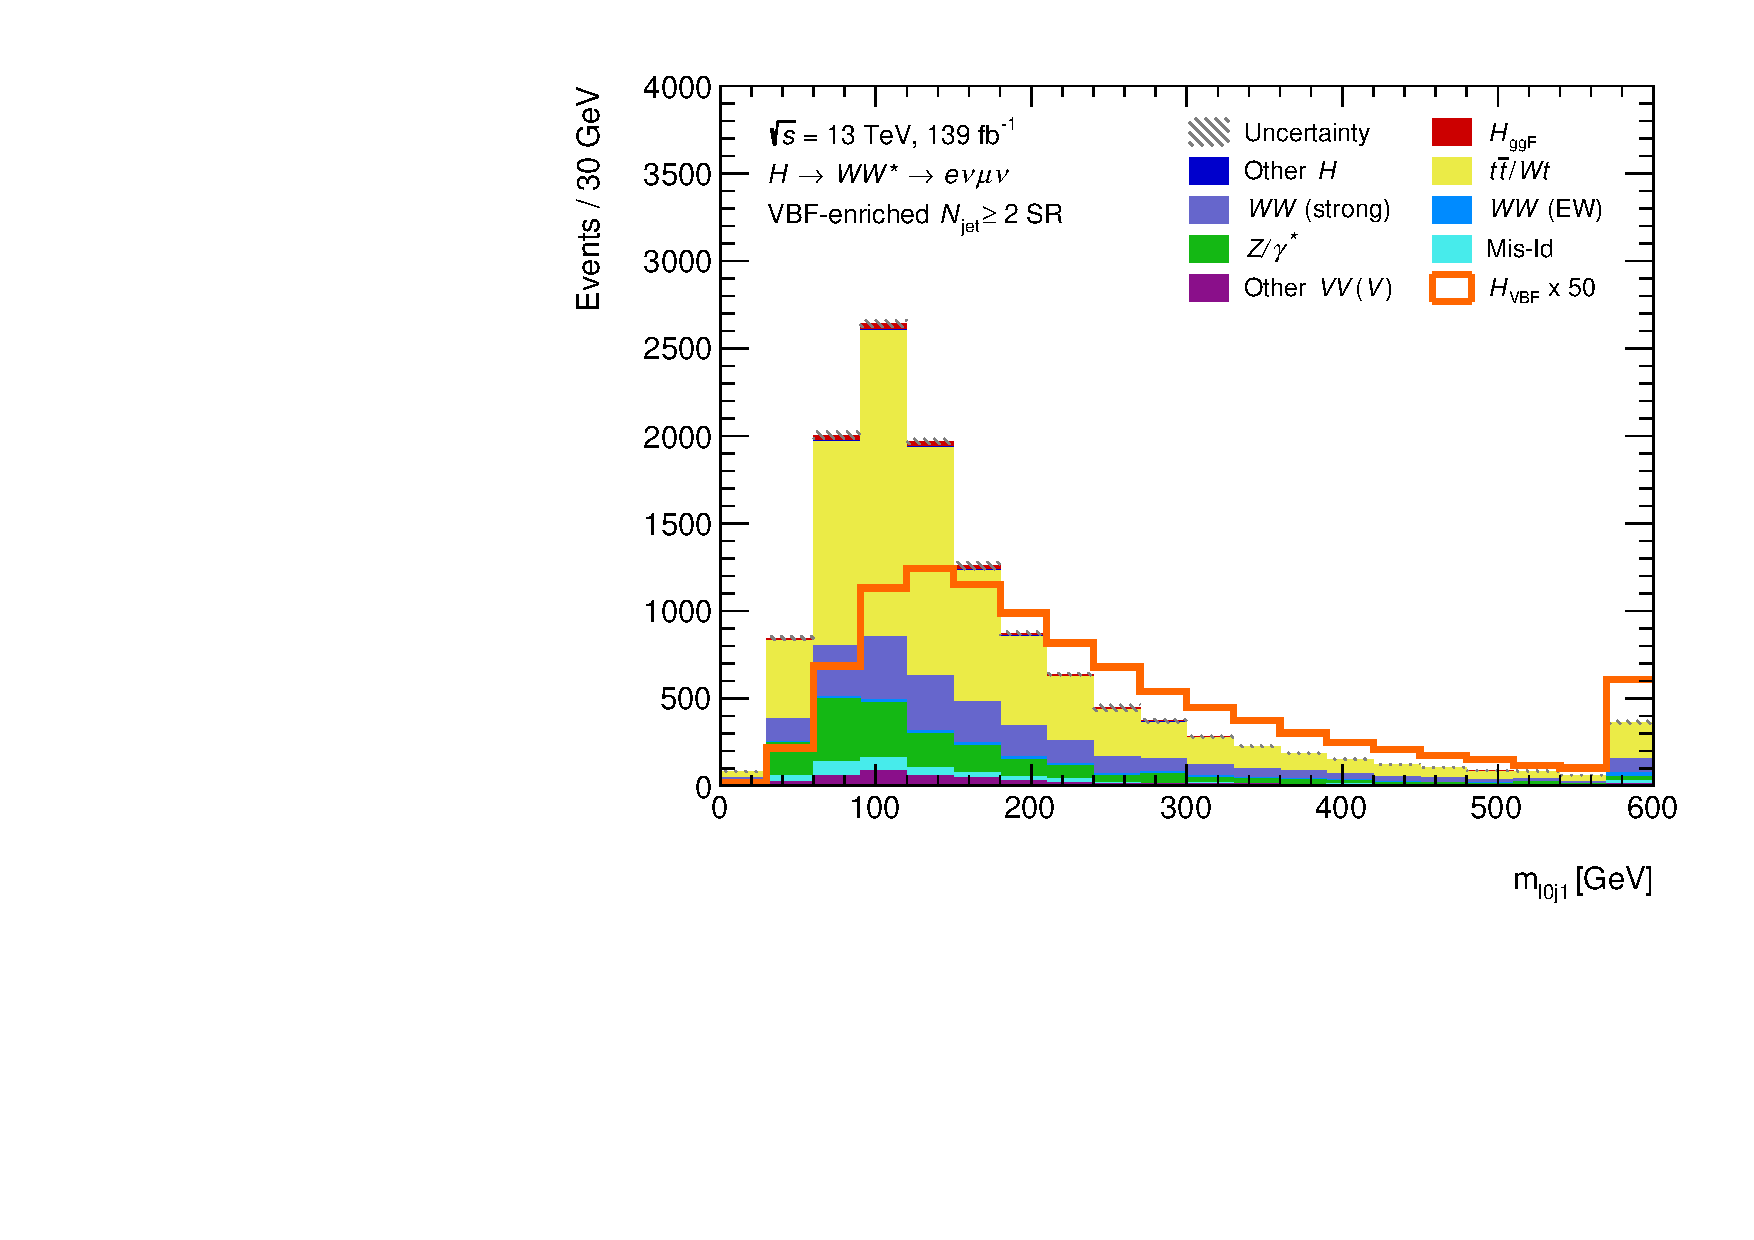
\includegraphics[width=0.32\textwidth]{figures/hww/dnn/blinded/run2-emme-CutVBF_SR-Ml0j1-lin.pdf} \hfill
        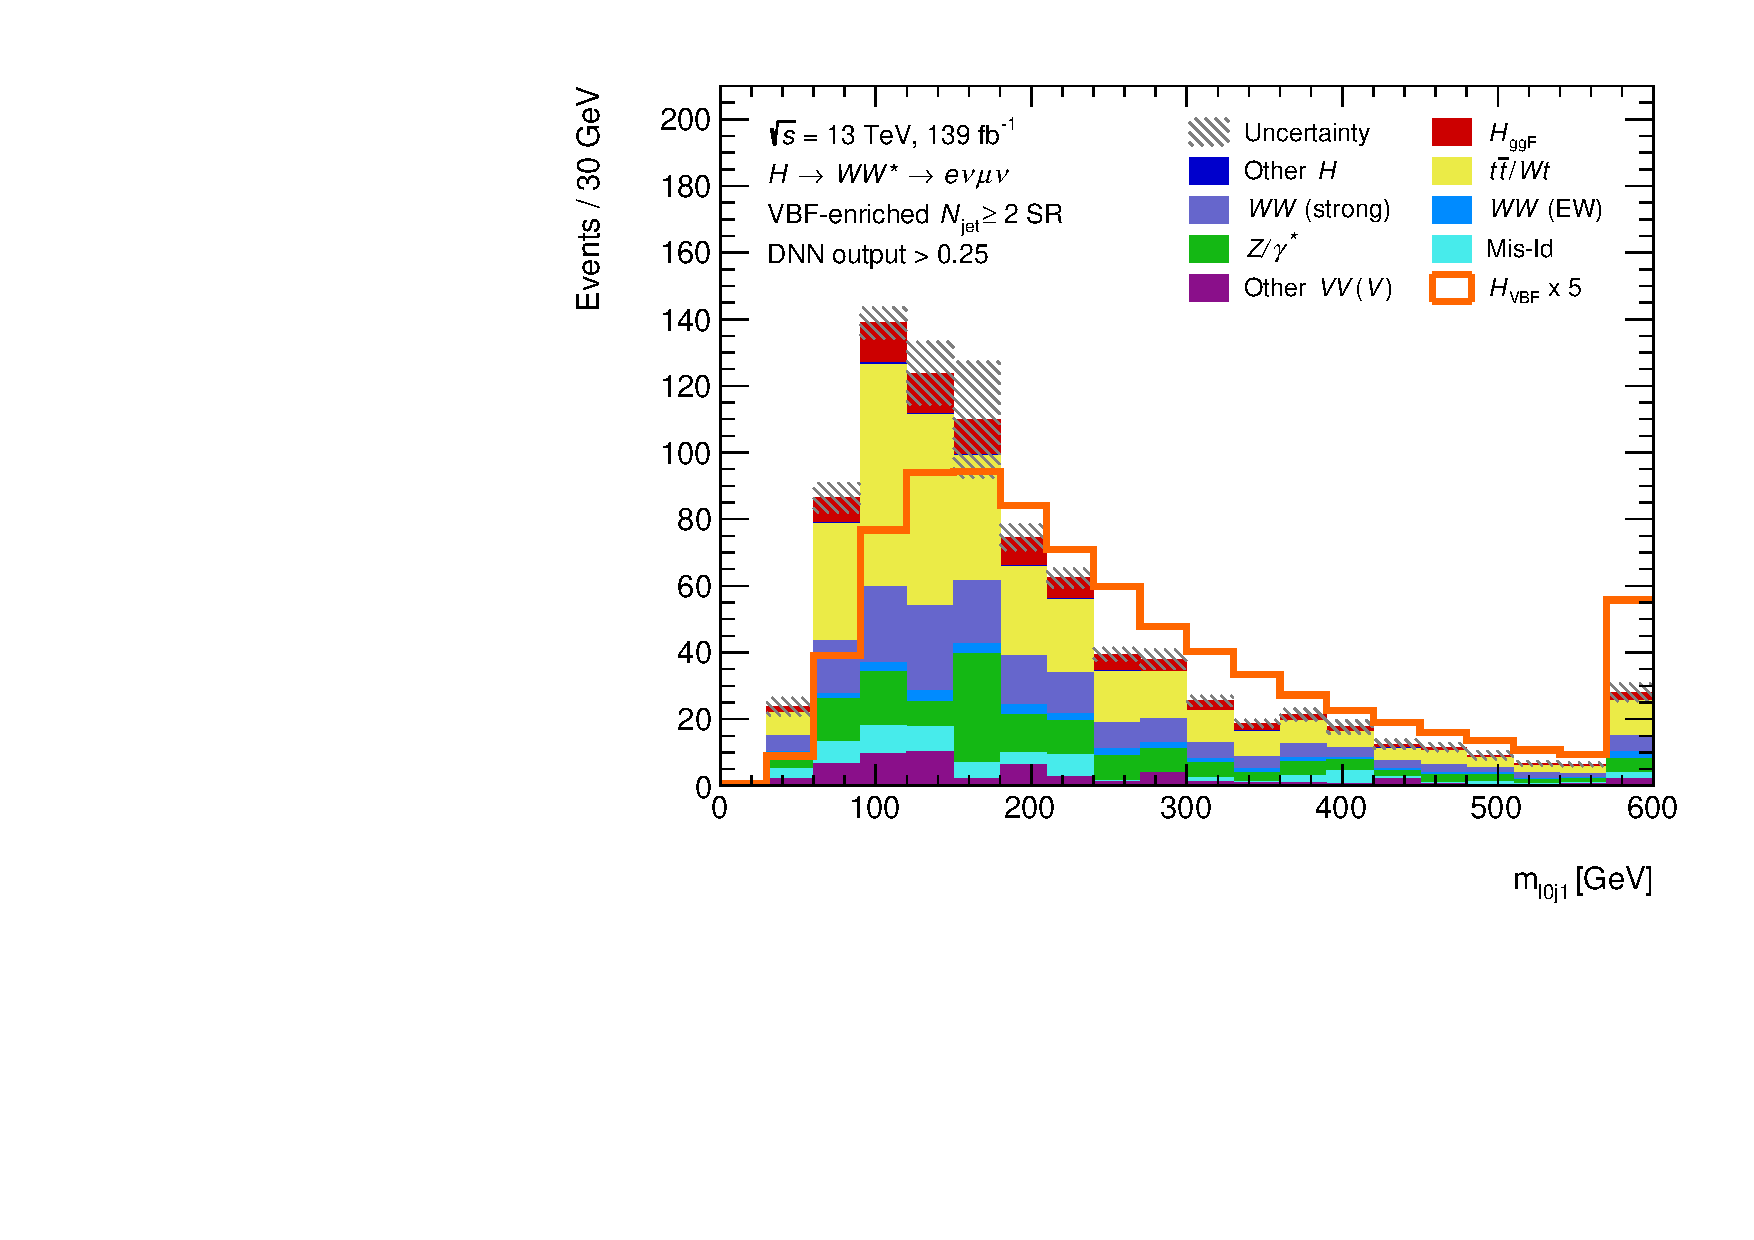
\includegraphics[width=0.32\textwidth]{figures/hww/dnn/blinded/run2-emme-CutVBFSR_DNN25-Ml0j1-lin.pdf} \hfill
        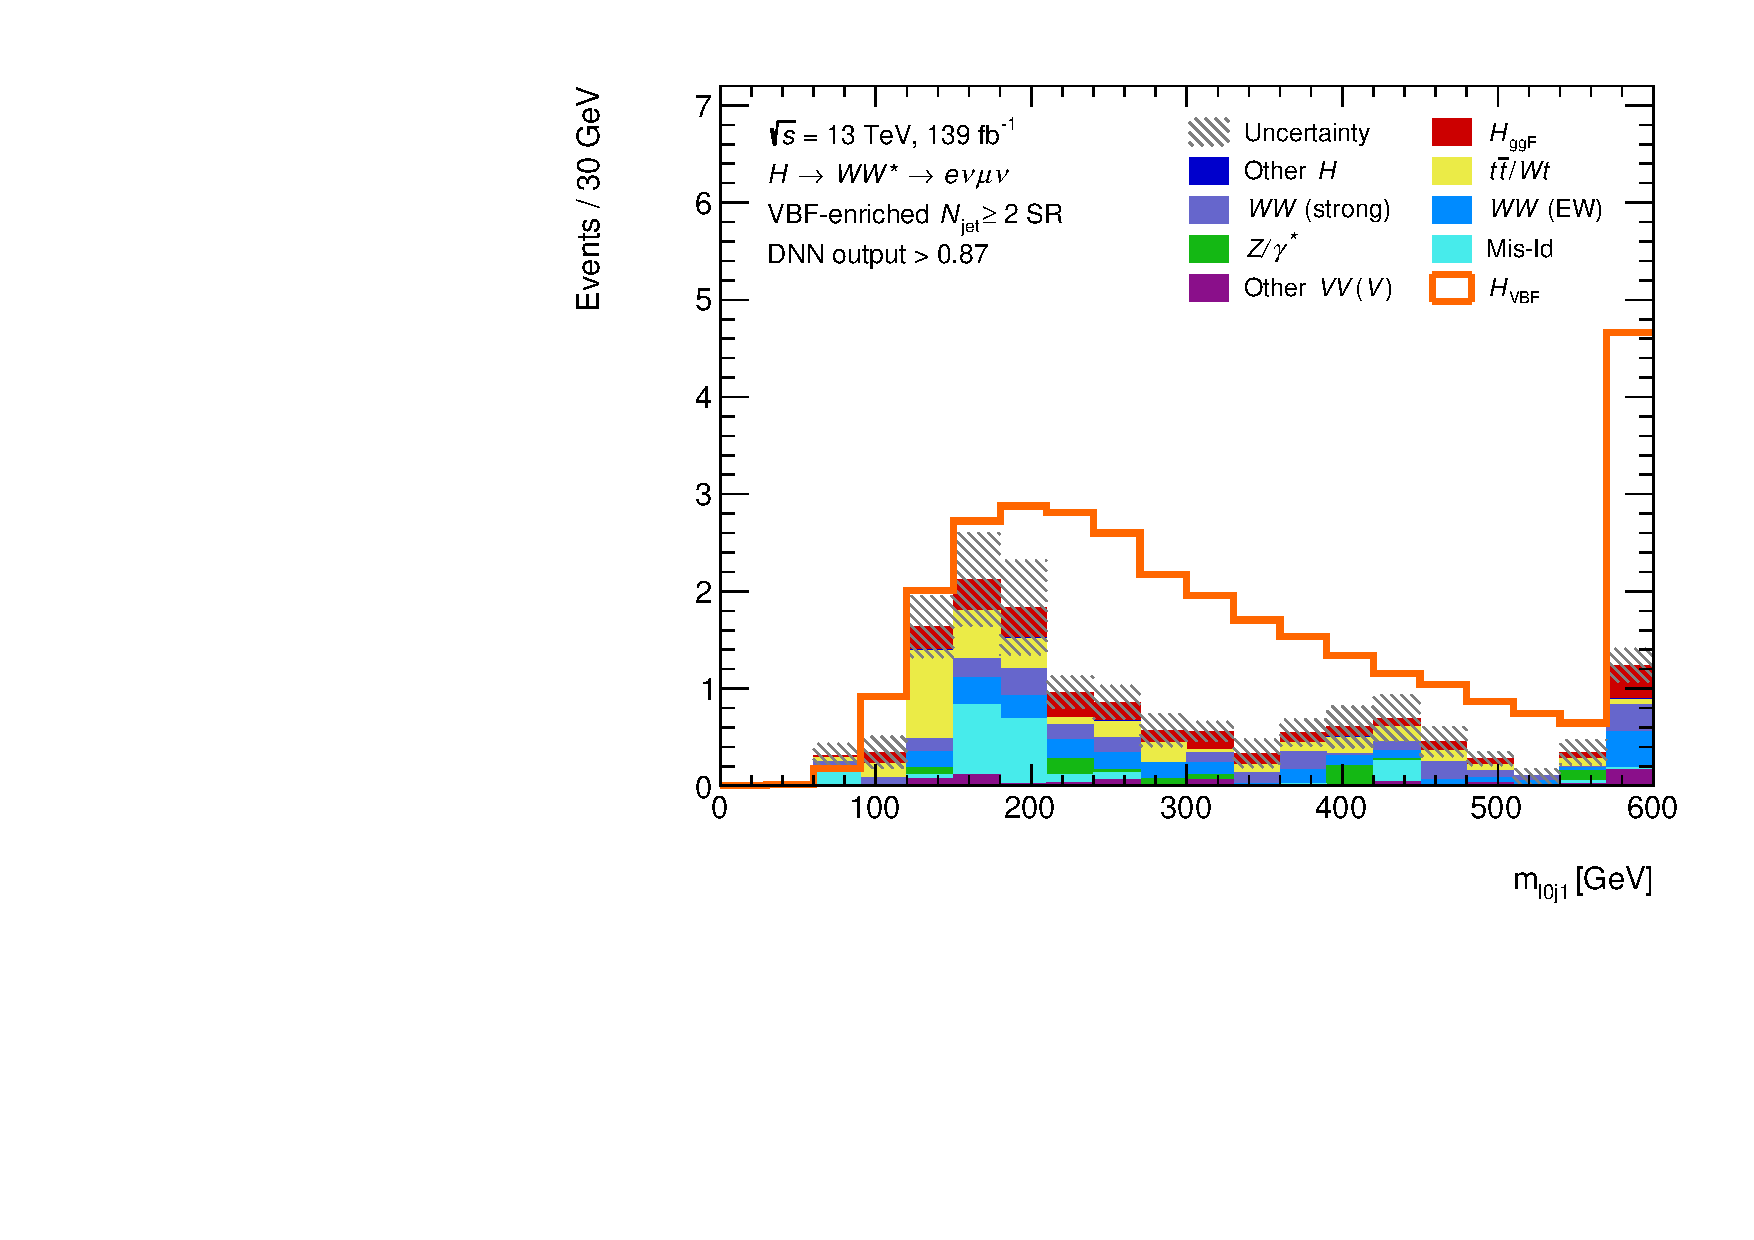
\includegraphics[width=0.32\textwidth]{figures/hww/dnn/blinded/run2-emme-CutVBFSR_DNN87-Ml0j1-lin.pdf}
    } \\
    \subfloat[$\mltwojtwo$]{
        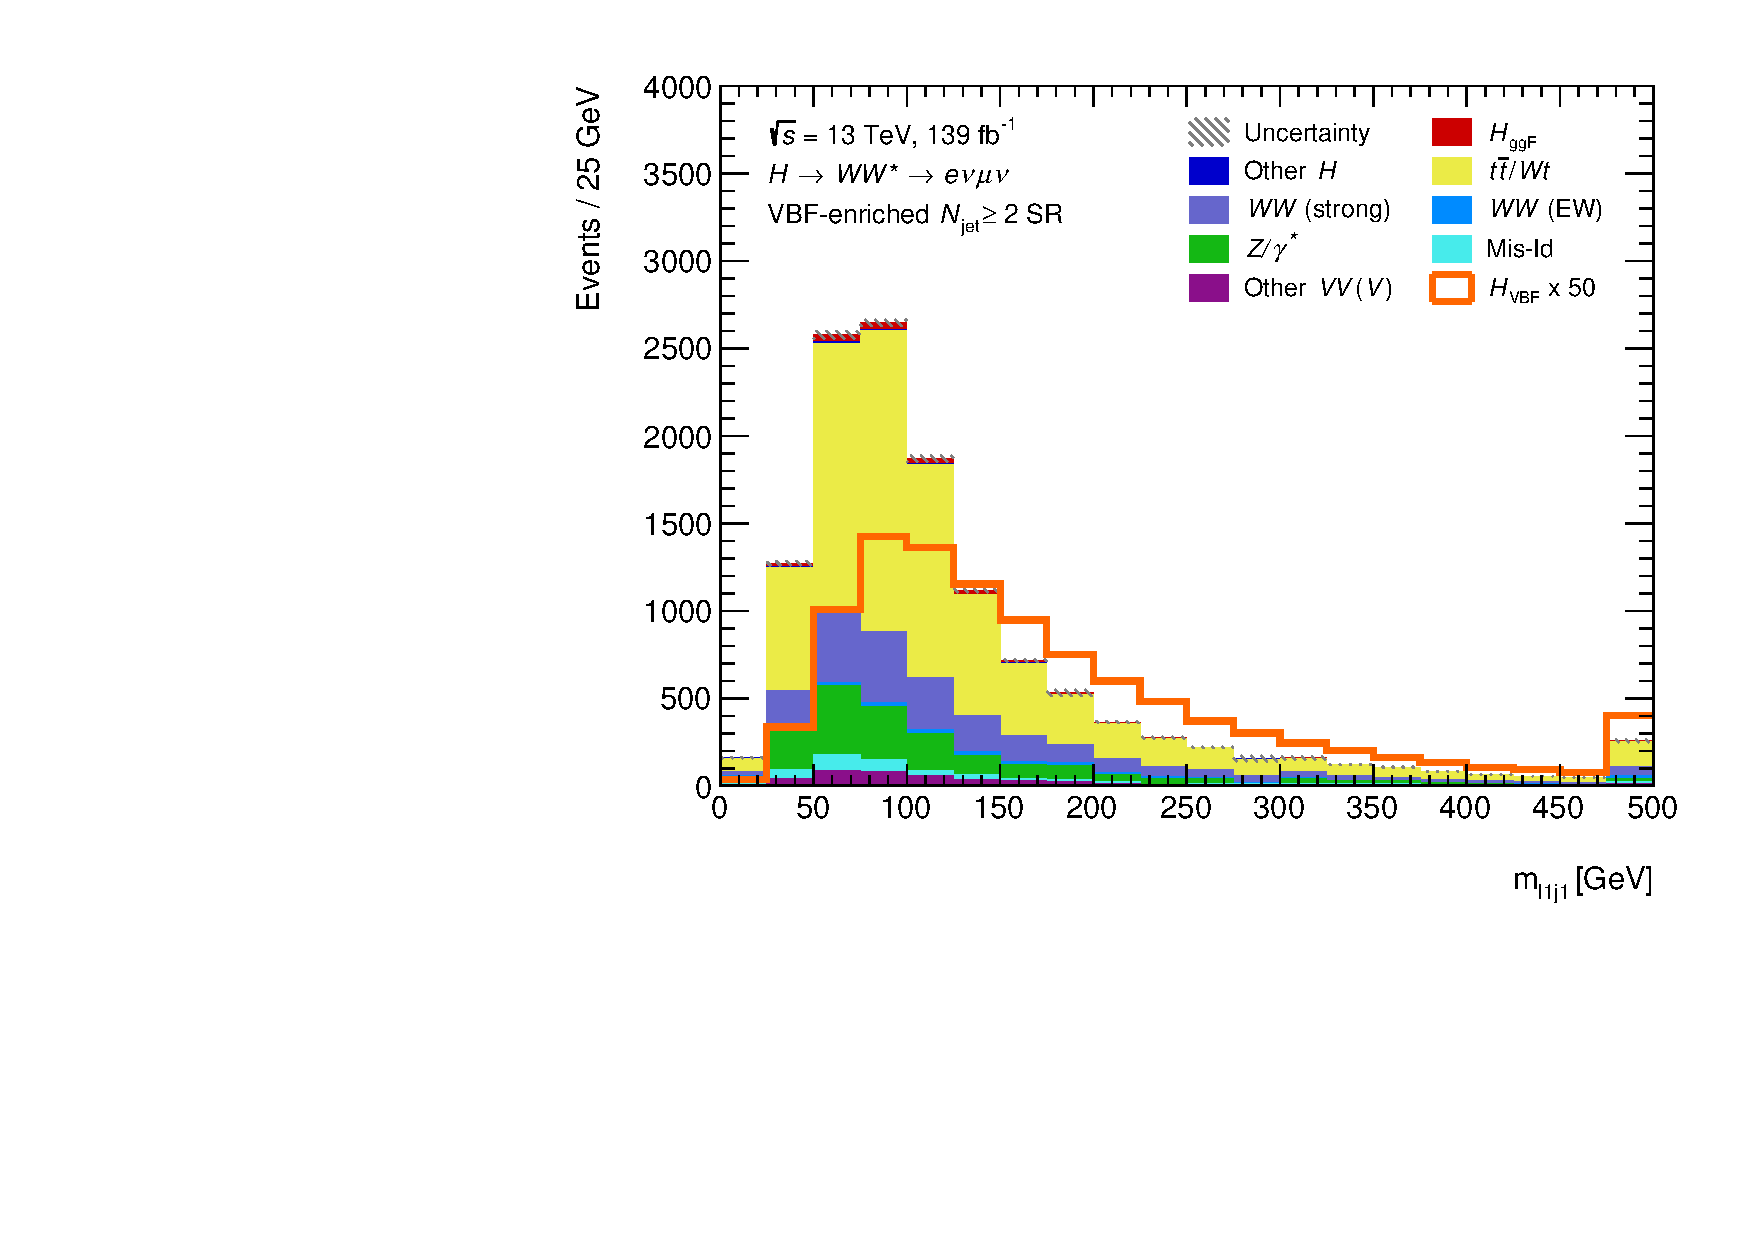
\includegraphics[width=0.32\textwidth]{figures/hww/dnn/blinded/run2-emme-CutVBF_SR-Ml1j1-lin.pdf} \hfill
        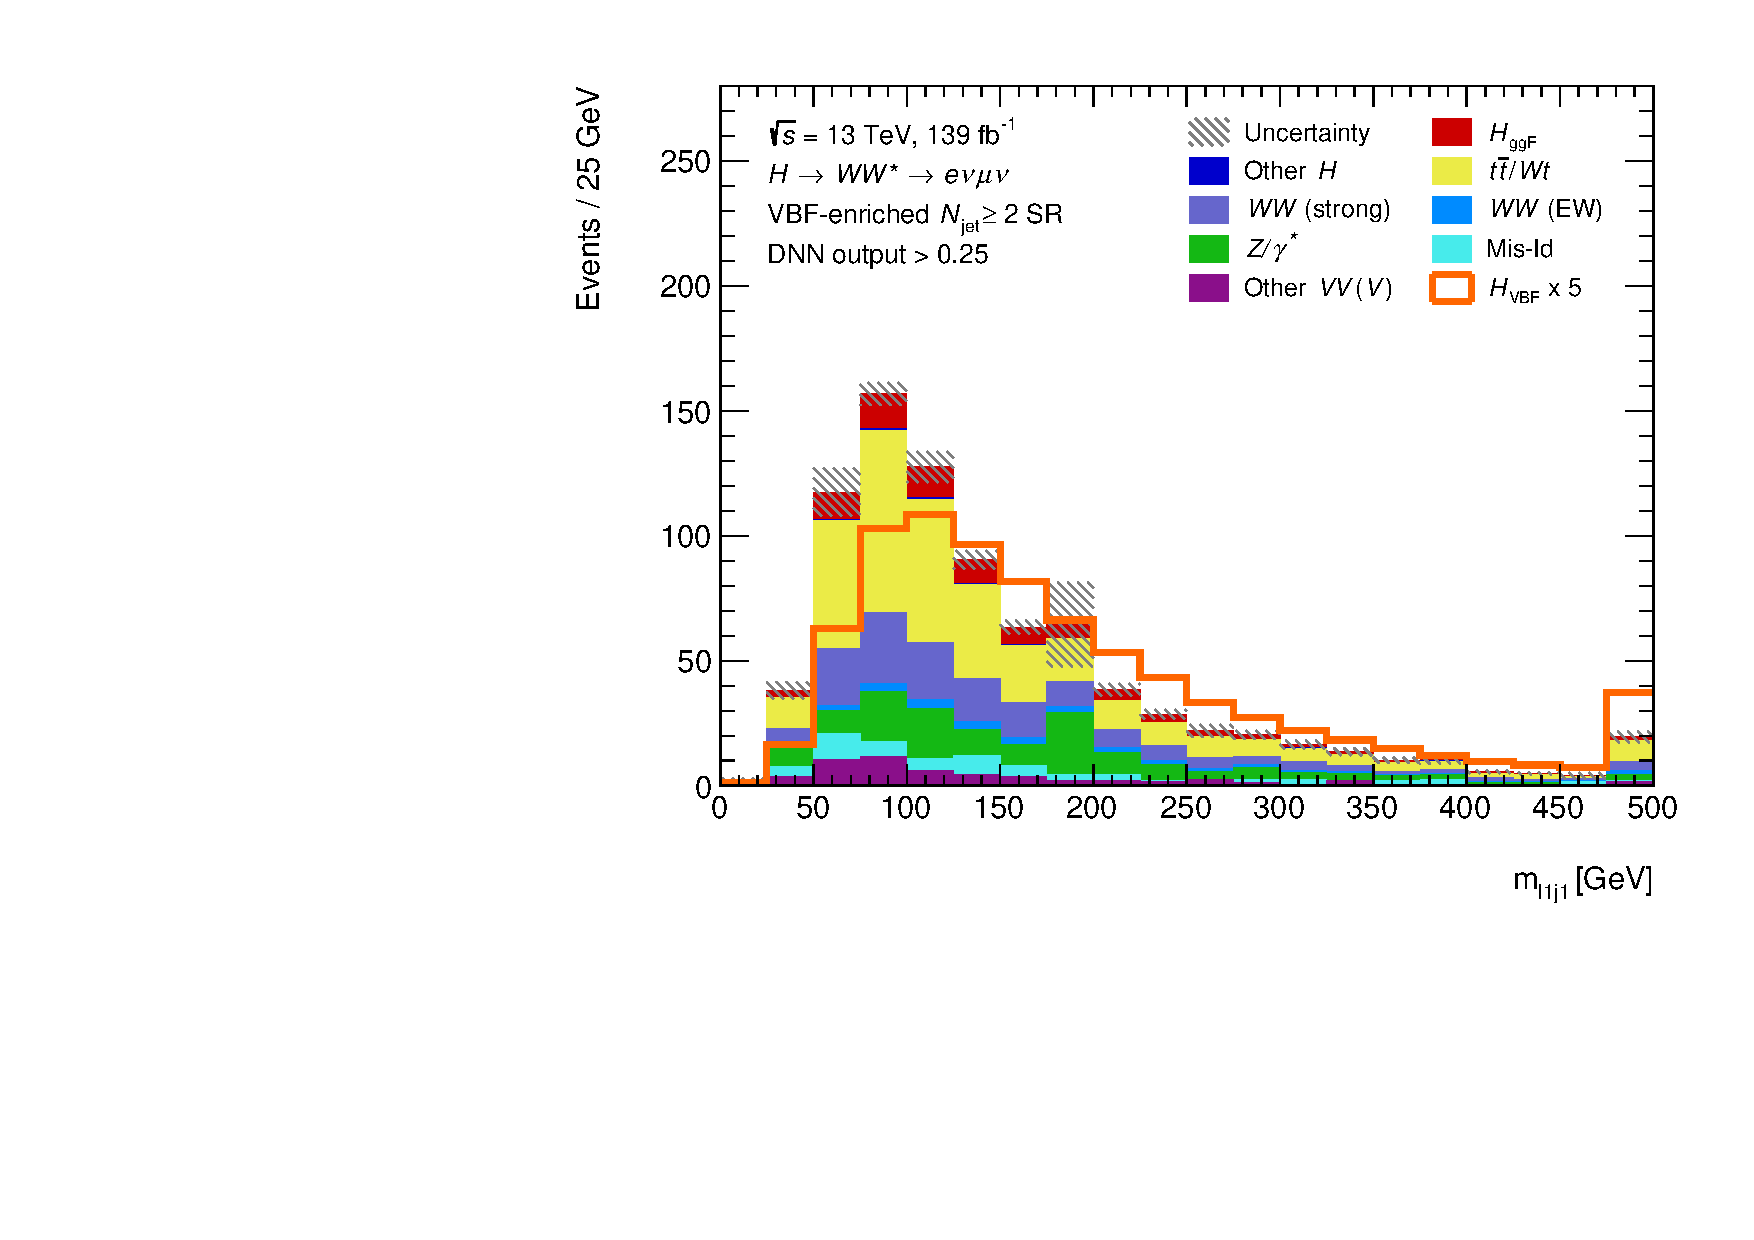
\includegraphics[width=0.32\textwidth]{figures/hww/dnn/blinded/run2-emme-CutVBFSR_DNN25-Ml1j1-lin.pdf} \hfill
        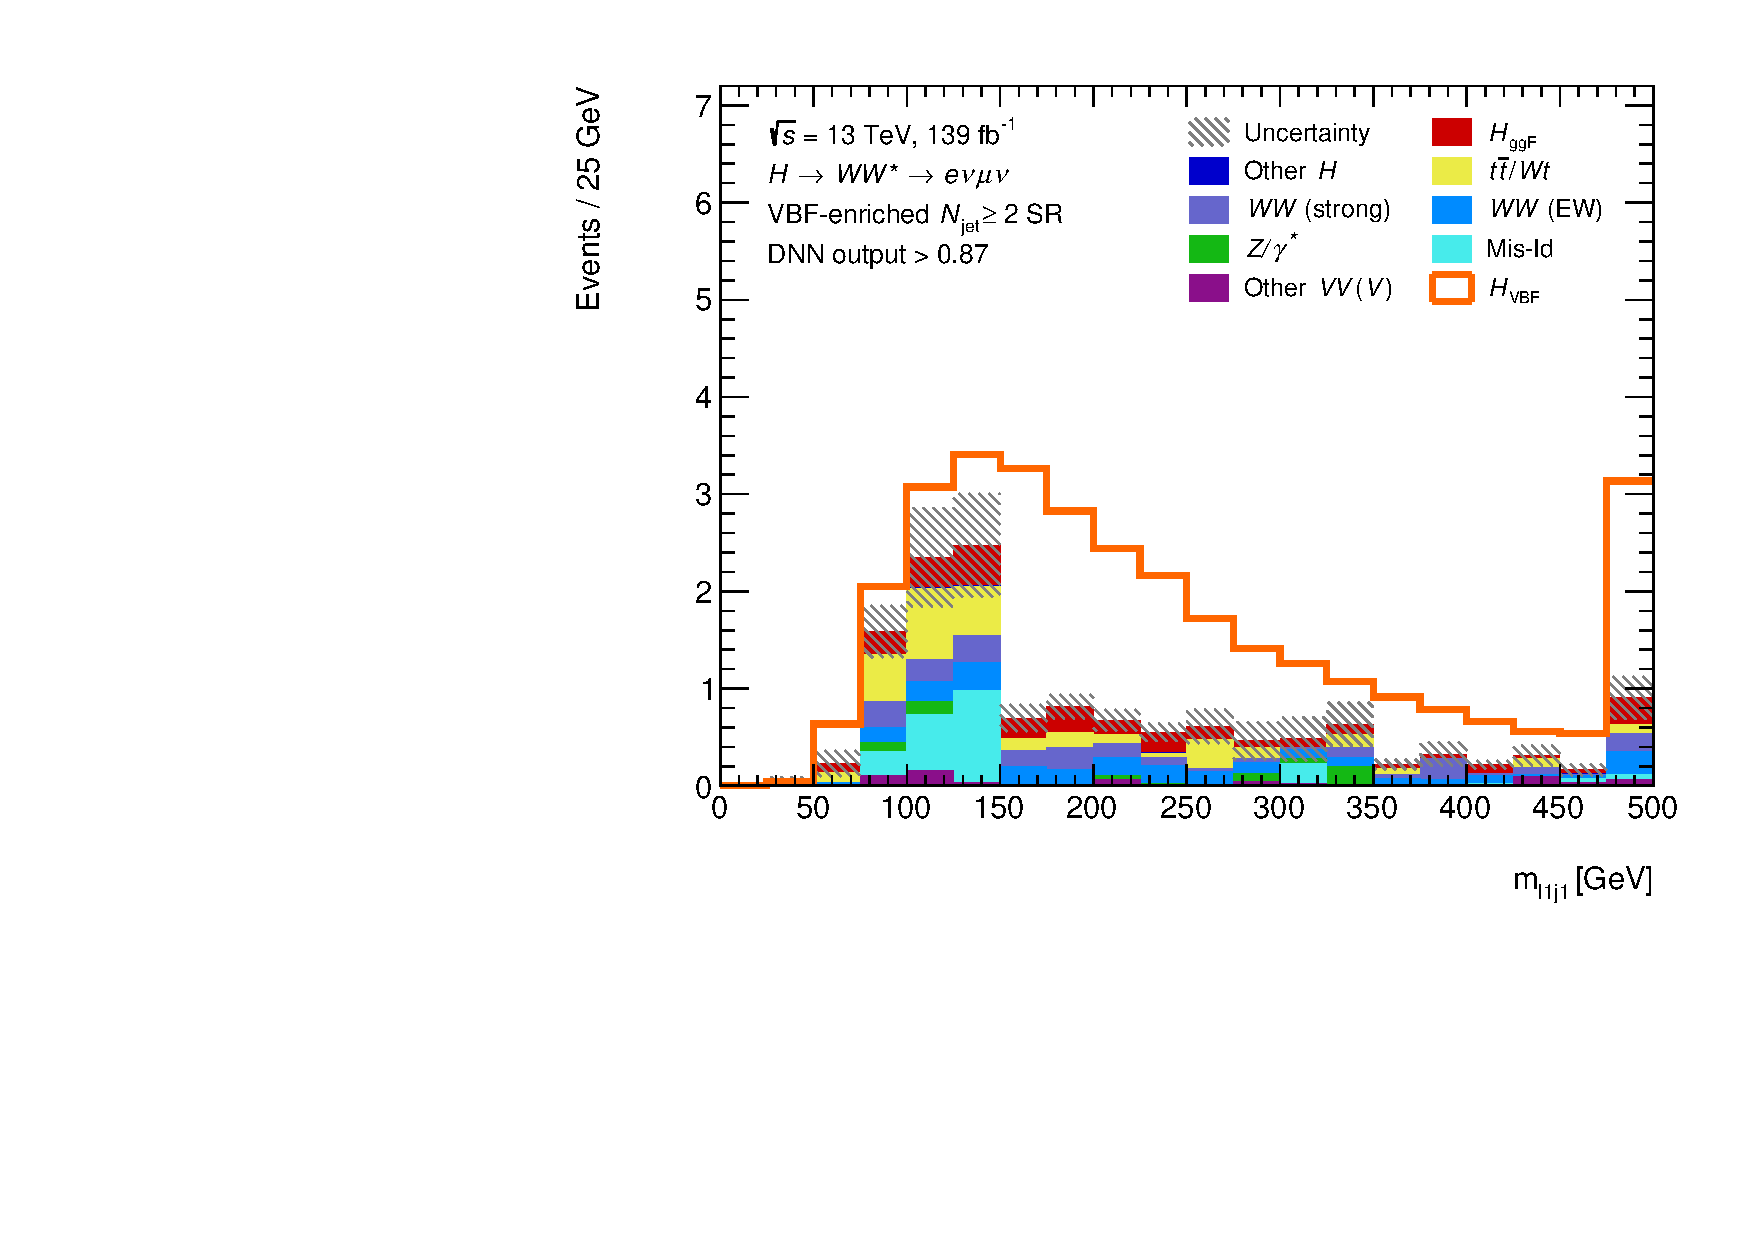
\includegraphics[width=0.32\textwidth]{figures/hww/dnn/blinded/run2-emme-CutVBFSR_DNN87-Ml1j1-lin.pdf}
    } 
    {\caption{Distributions of $\mlonejone$, $\mltwojone$, $\mlonejtwo$, and $\mltwojtwo$ in the VBF signal region.
            Each row shows one variable with different cuts on the DNN output distribution being applied in different columns.
            \label{app:fig:dnn-inputs-vbf-top2} }}
\end{figure}


\begin{figure}[h]
    \centering
    \subfloat[$\pTjone$]{
        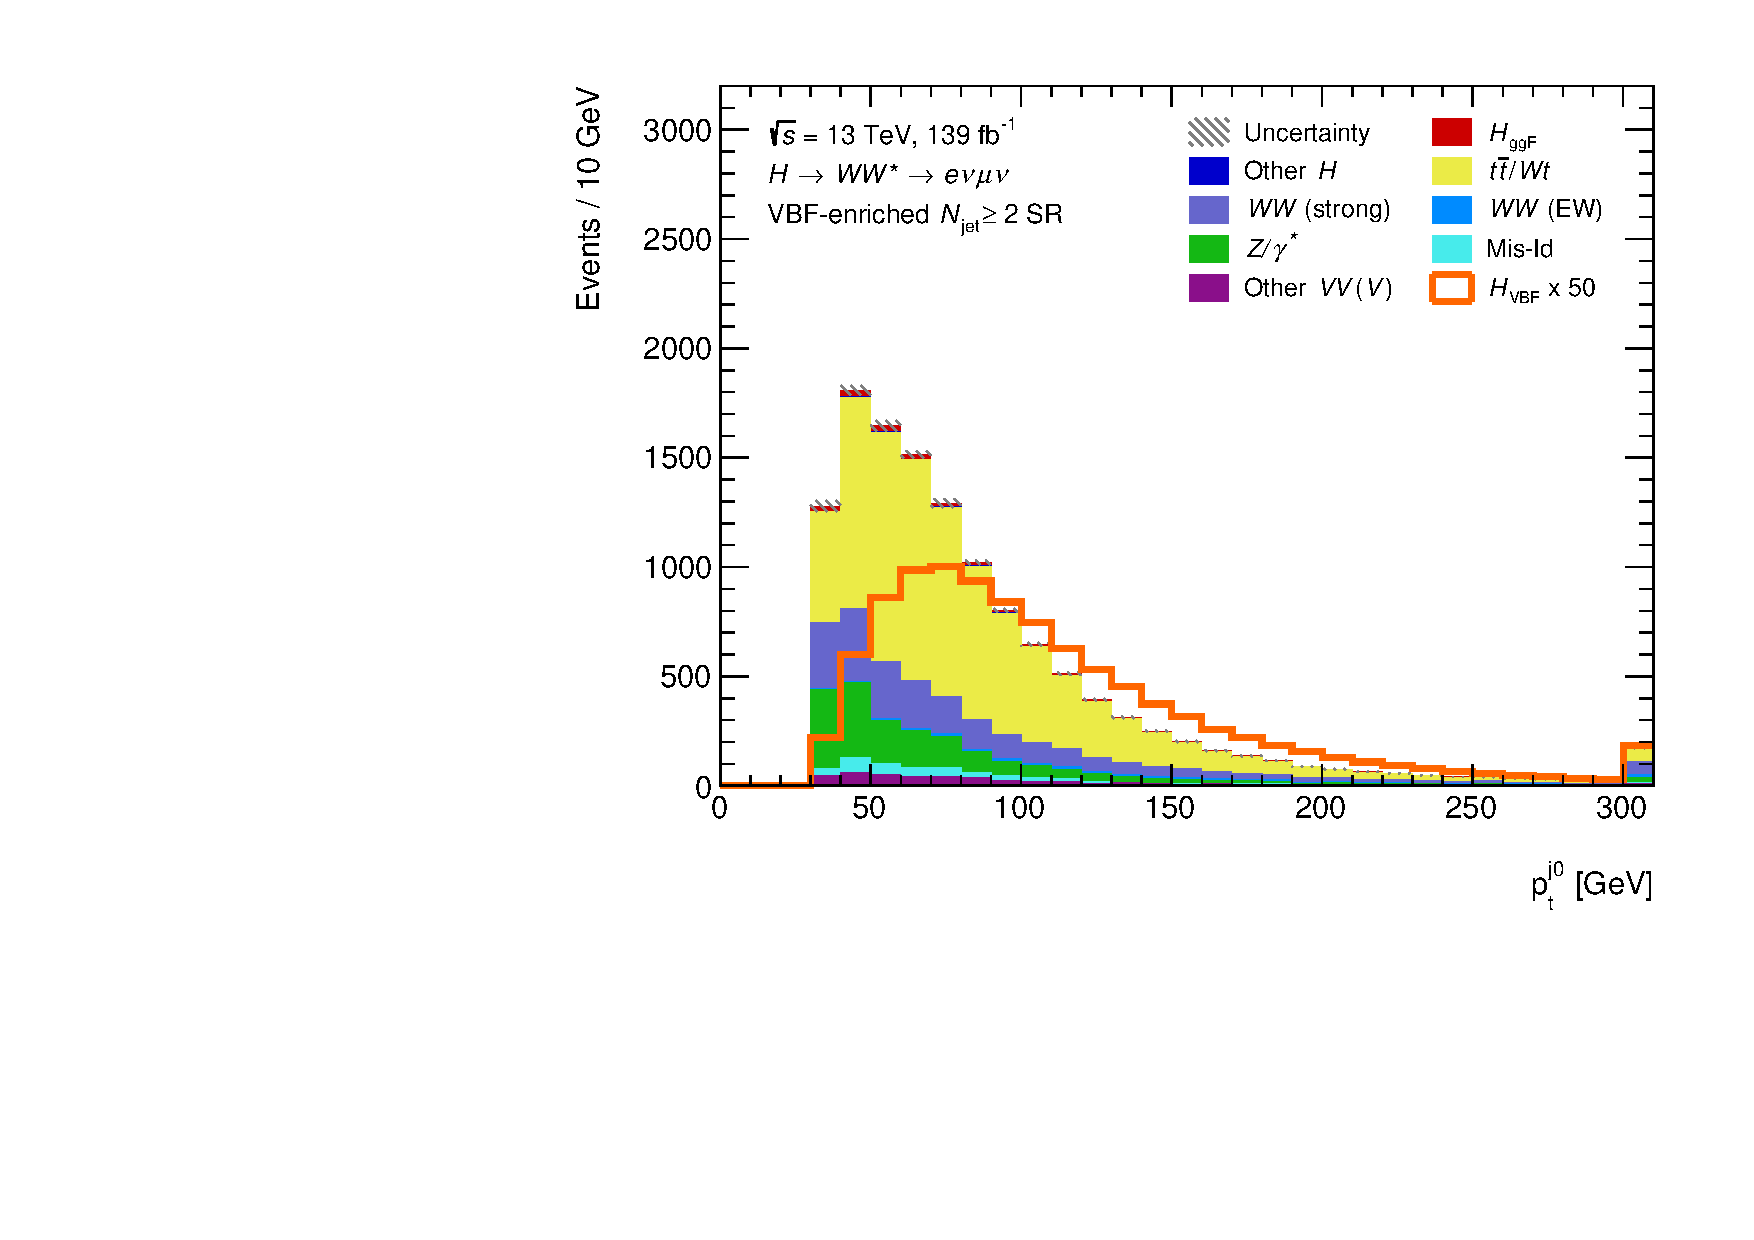
\includegraphics[width=0.32\textwidth]{figures/hww/dnn/blinded/run2-emme-CutVBF_SR-leadJetPt-lin.pdf} \hfill
        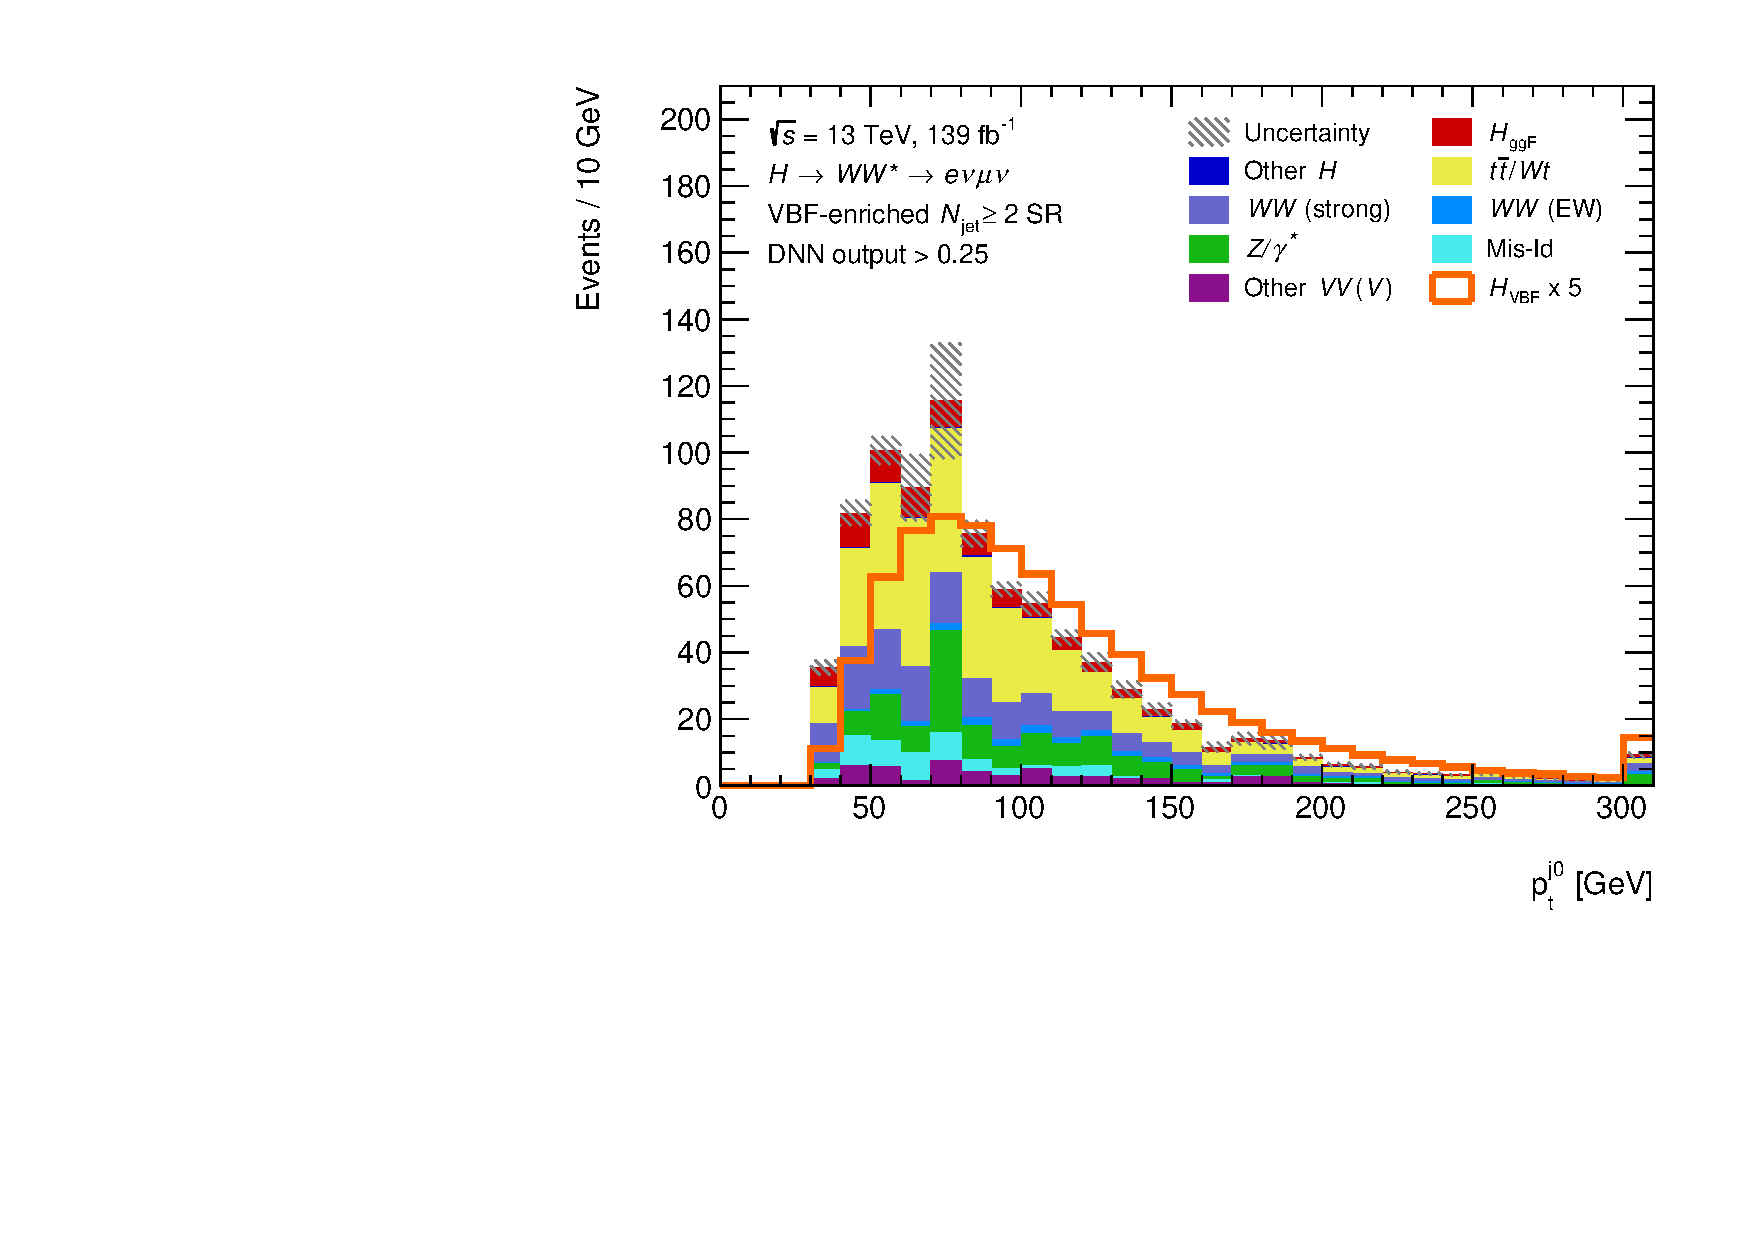
\includegraphics[width=0.32\textwidth]{figures/hww/dnn/blinded/run2-emme-CutVBFSR_DNN25-leadJetPt-lin.pdf} \hfill
        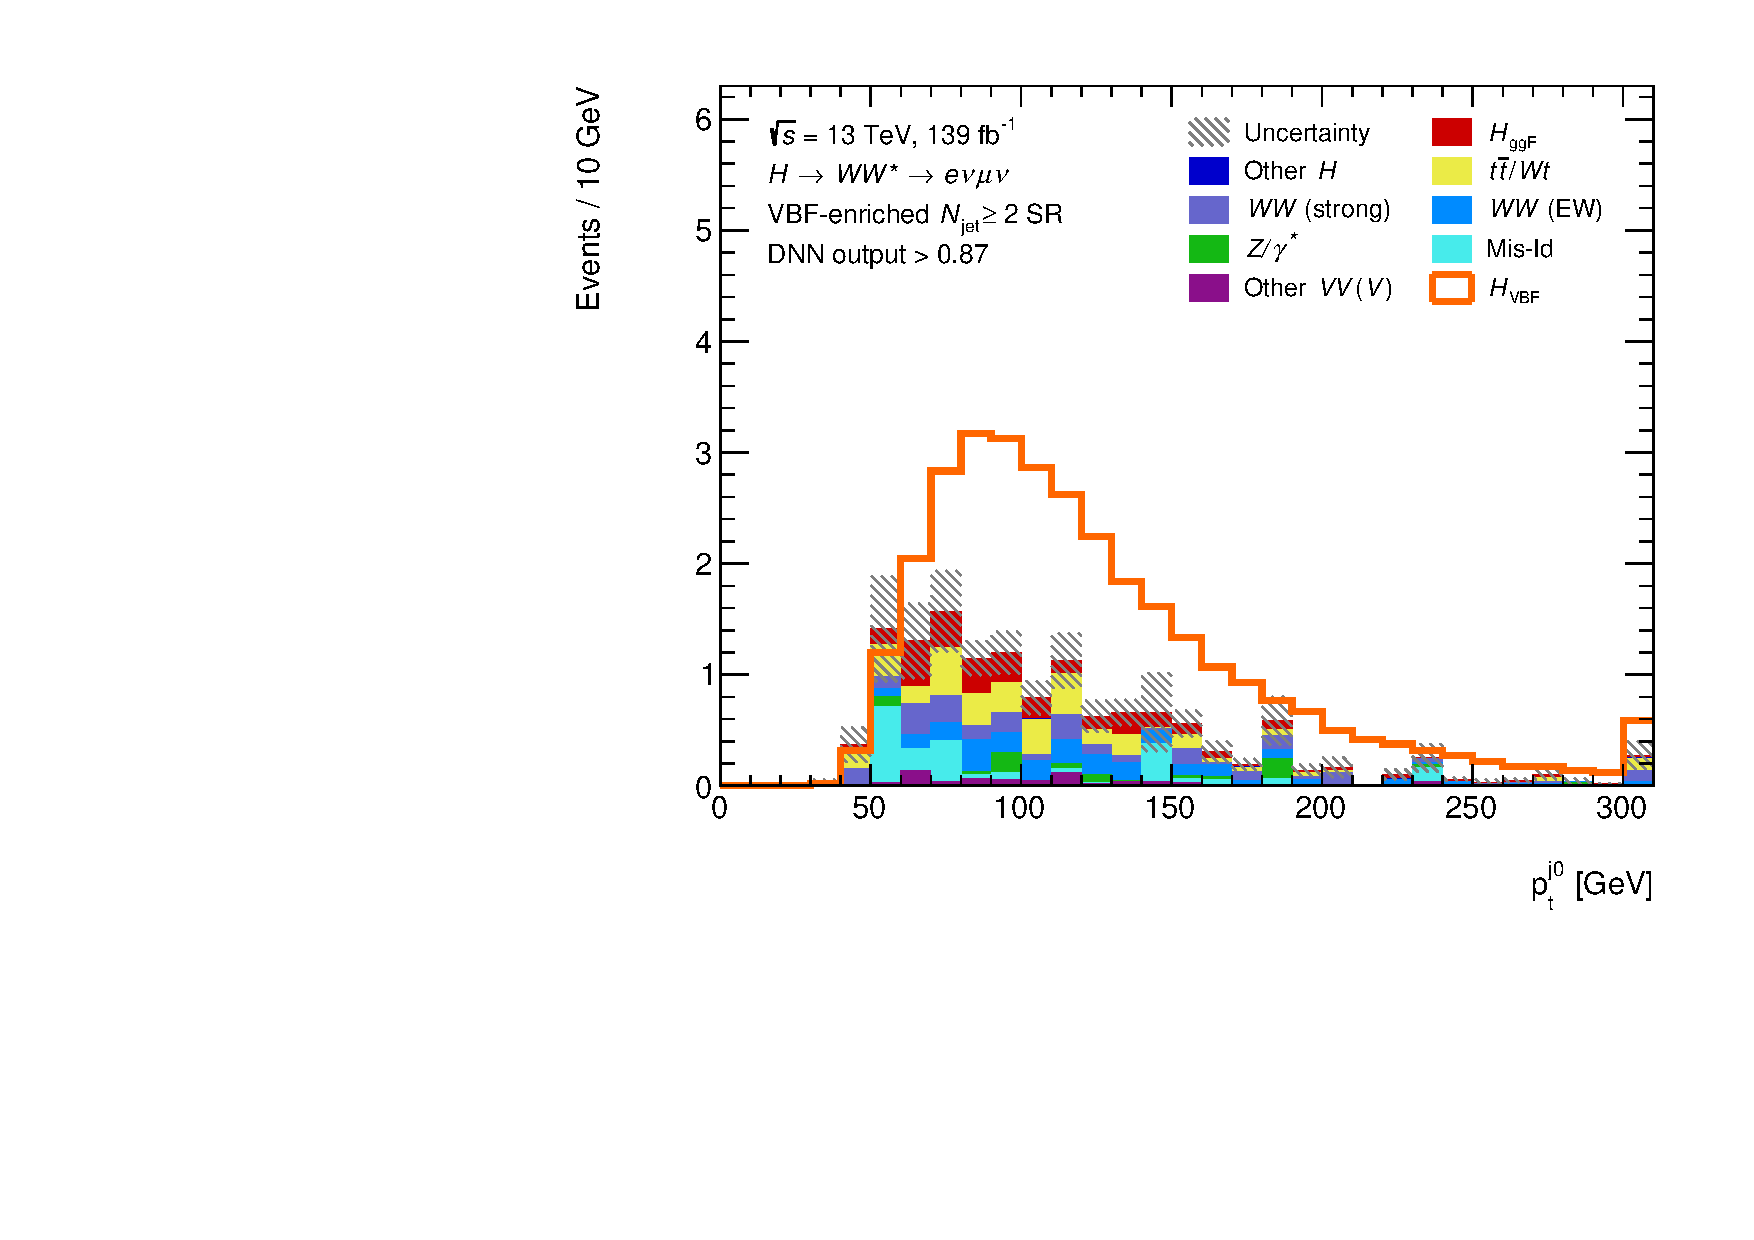
\includegraphics[width=0.32\textwidth]{figures/hww/dnn/blinded/run2-emme-CutVBFSR_DNN87-leadJetPt-lin.pdf}
    } \\
    \subfloat[$\pTjtwo$]{
        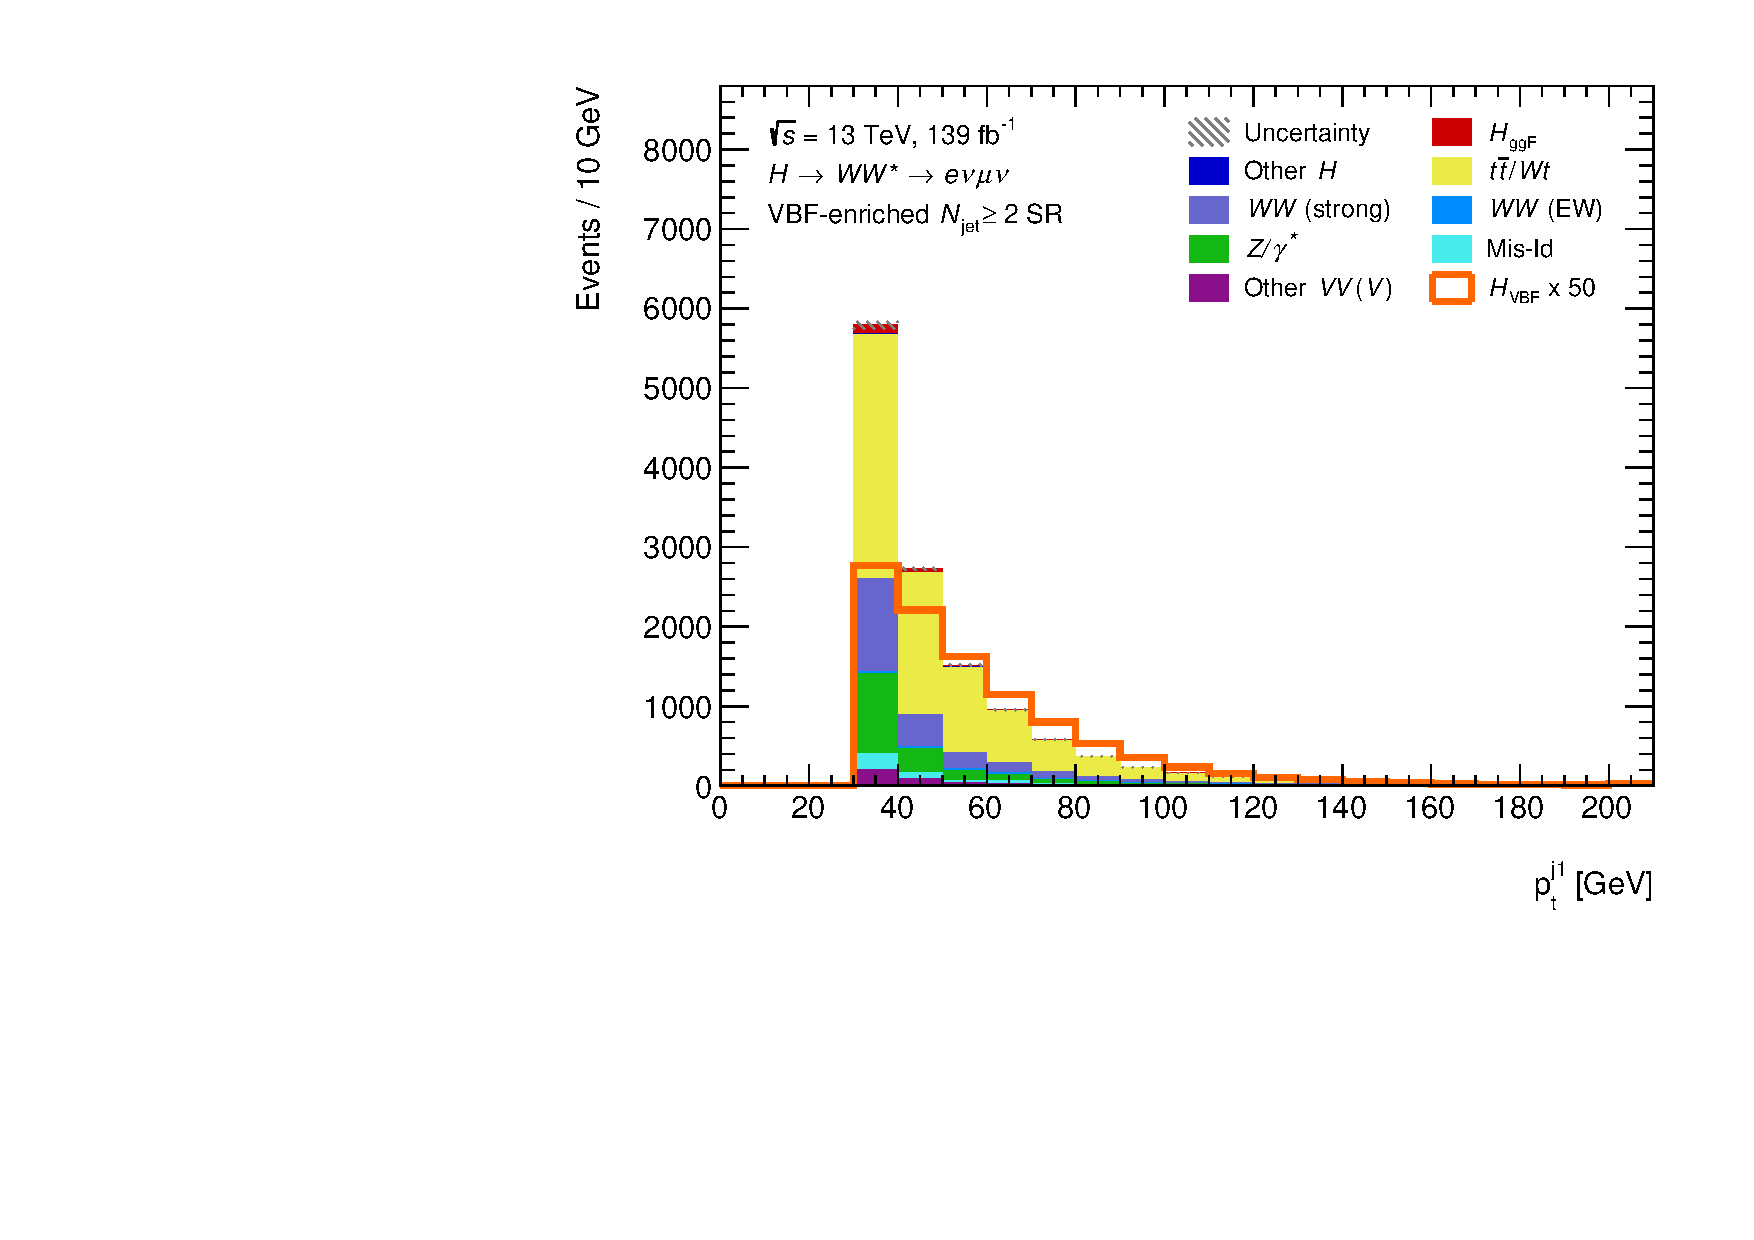
\includegraphics[width=0.32\textwidth]{figures/hww/dnn/blinded/run2-emme-CutVBF_SR-subleadJetPt-lin.pdf} \hfill
        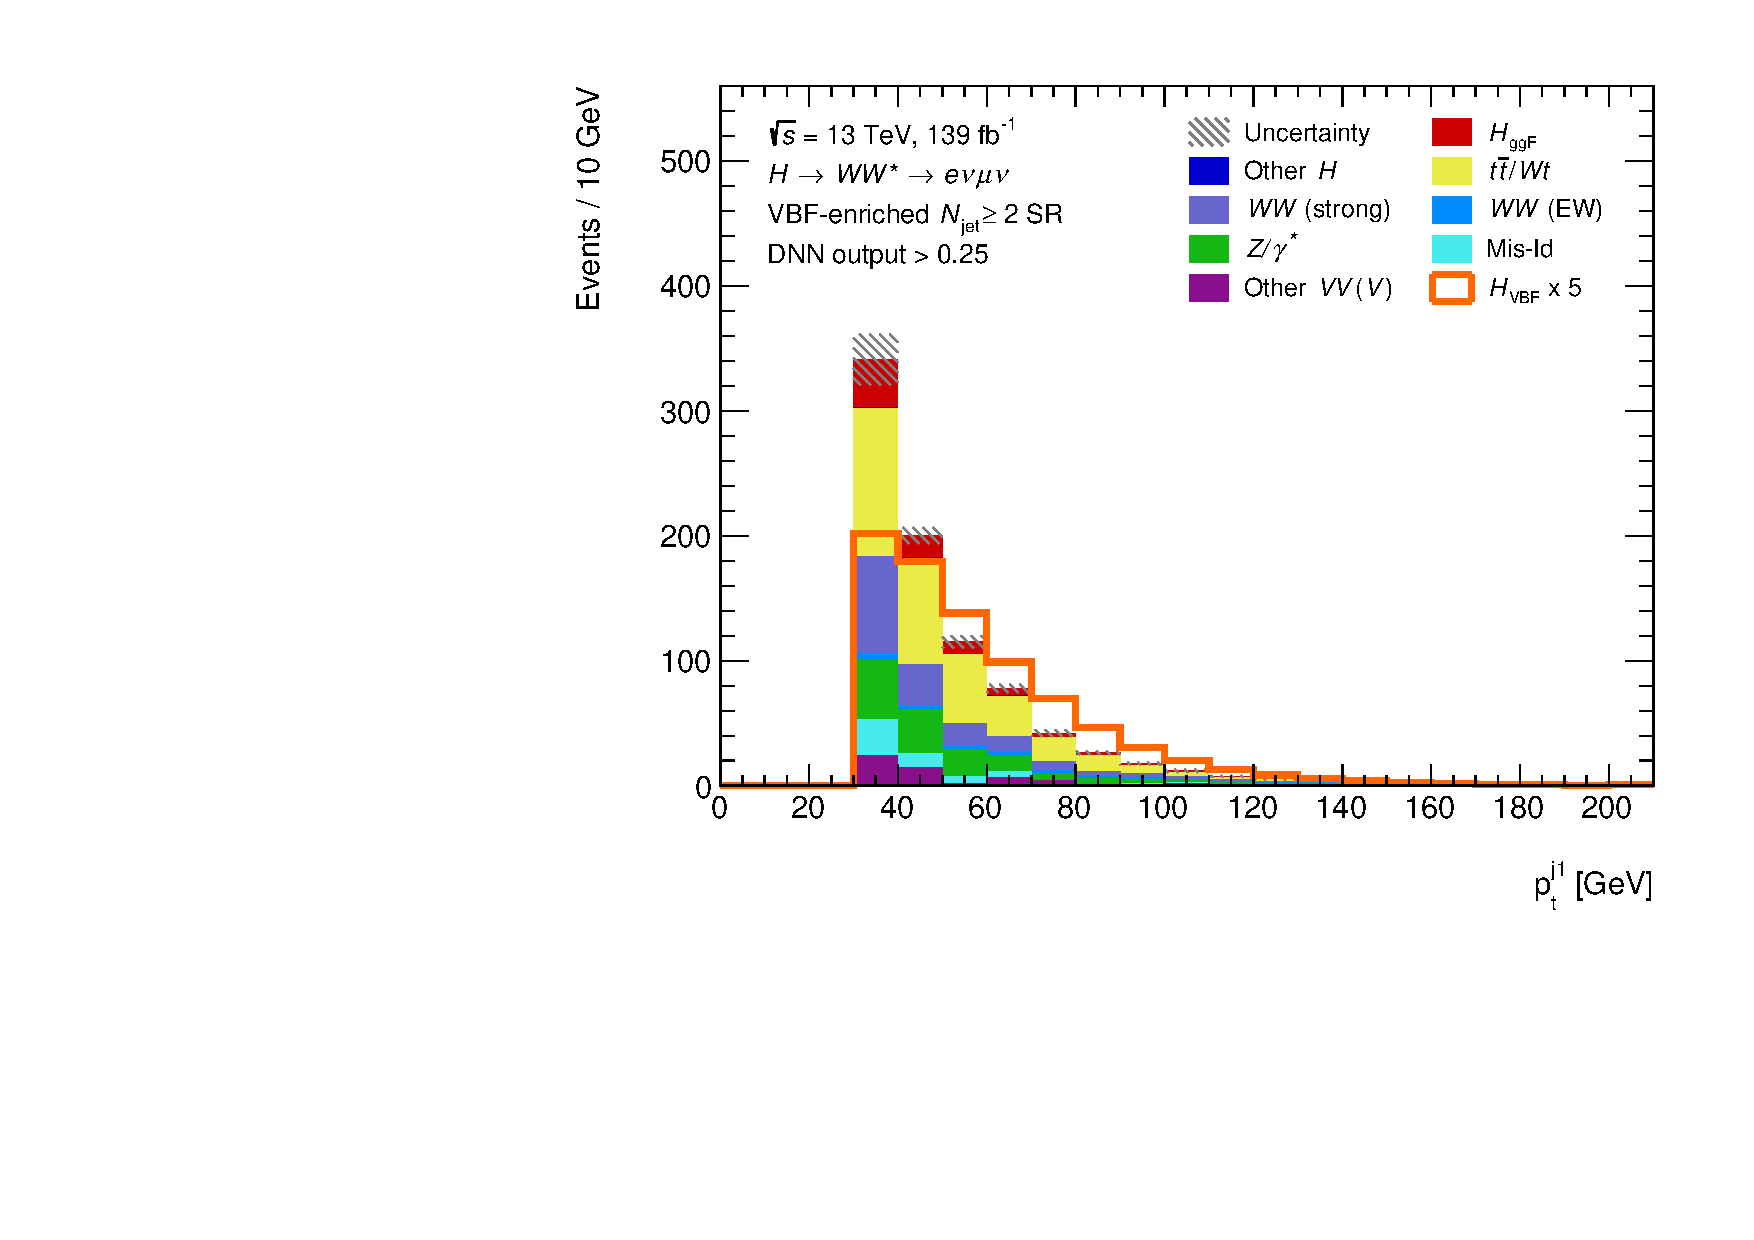
\includegraphics[width=0.32\textwidth]{figures/hww/dnn/blinded/run2-emme-CutVBFSR_DNN25-subleadJetPt-lin.pdf} \hfill
        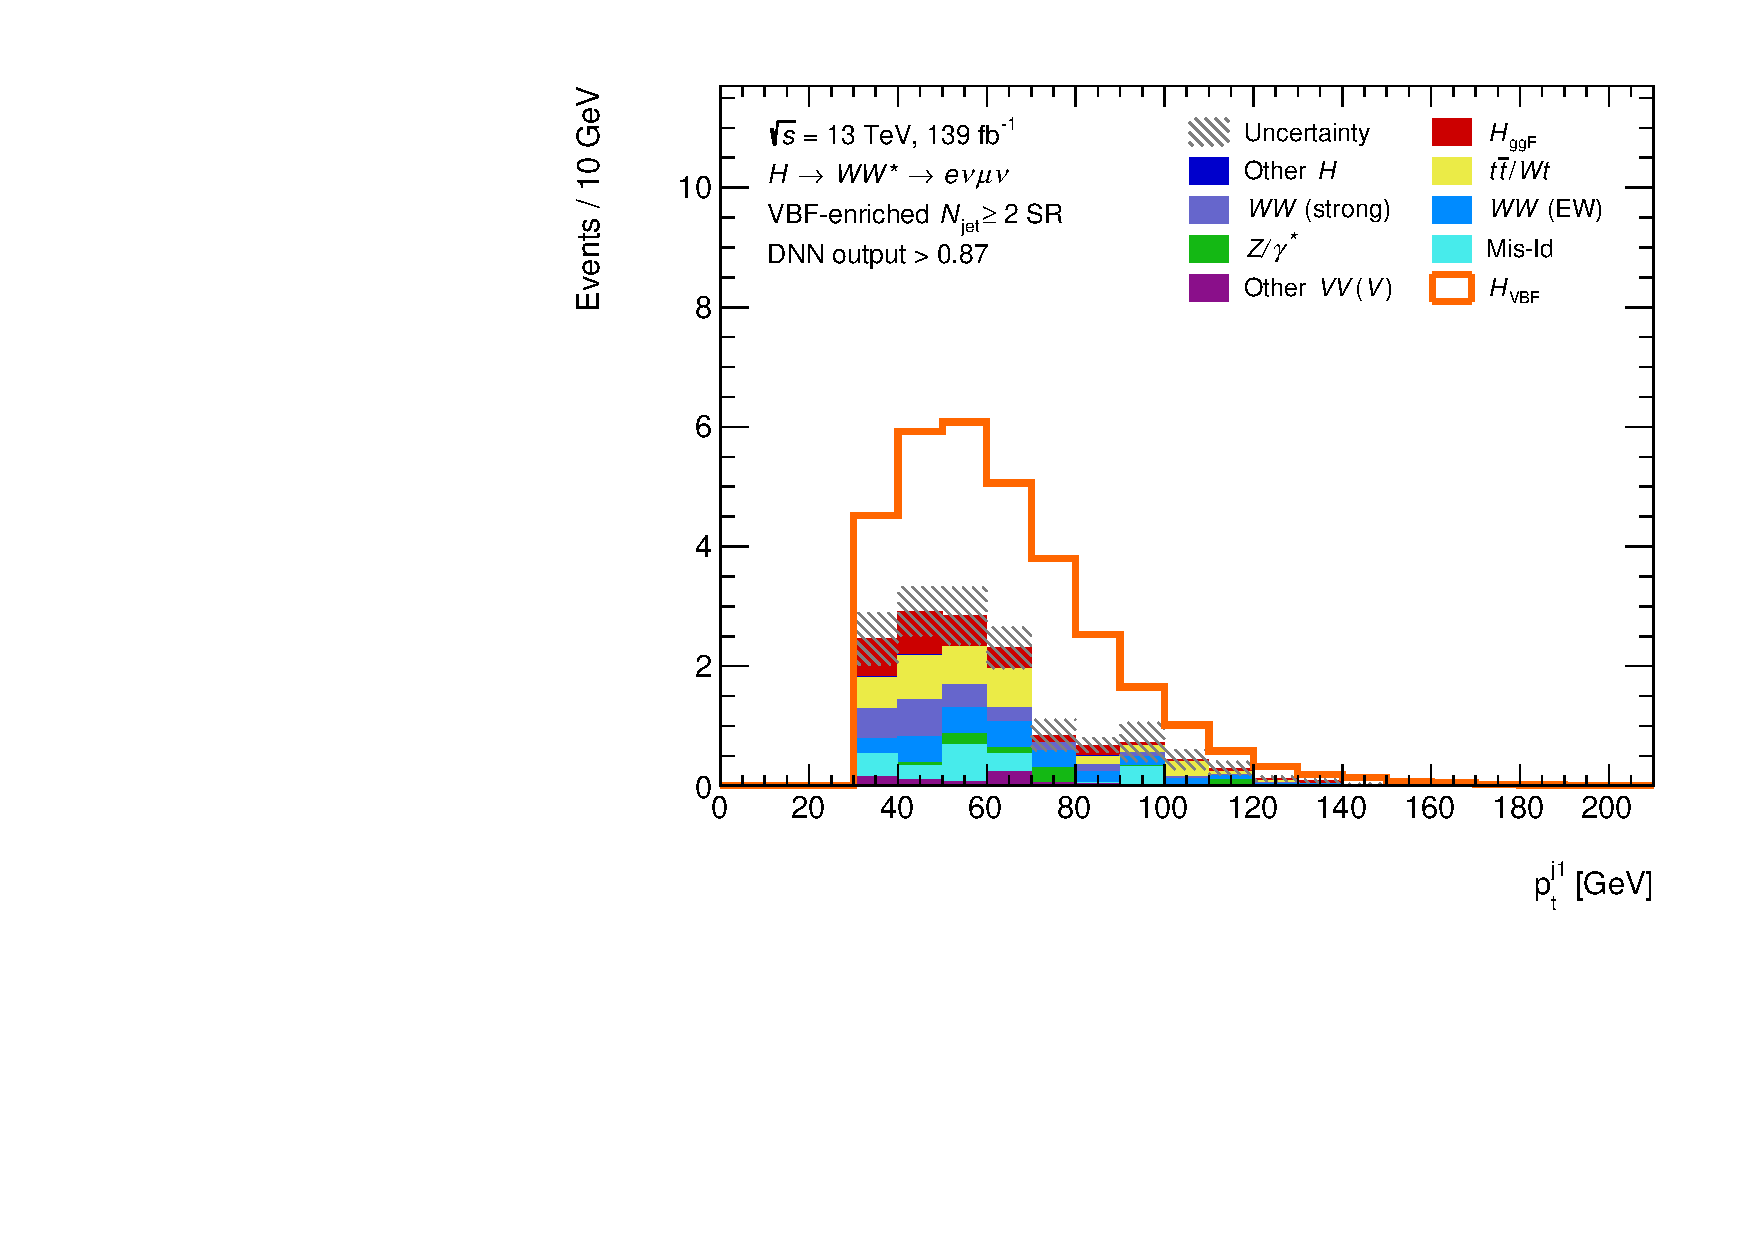
\includegraphics[width=0.32\textwidth]{figures/hww/dnn/blinded/run2-emme-CutVBFSR_DNN87-subleadJetPt-lin.pdf}
    } \\
    \subfloat[$\pTjthree$]{
        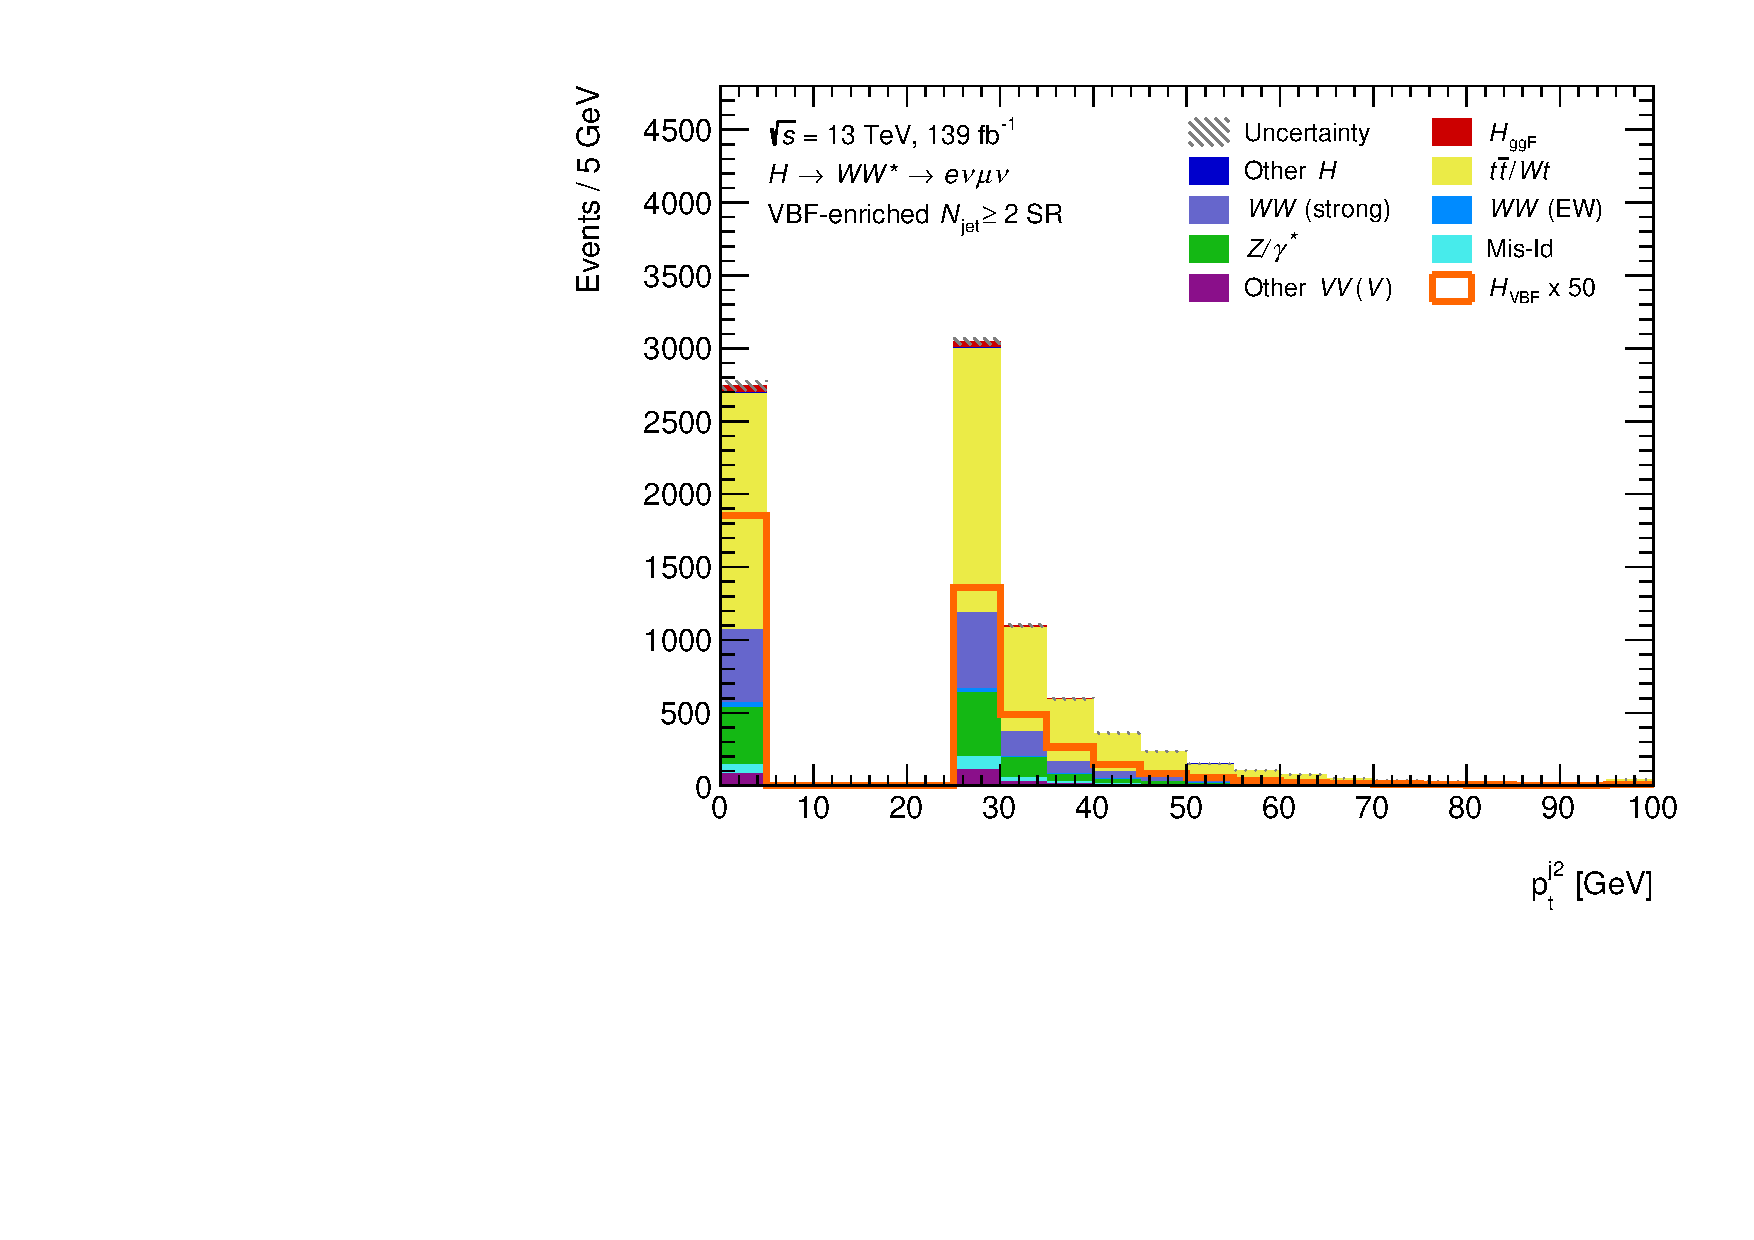
\includegraphics[width=0.32\textwidth]{figures/hww/dnn/blinded/run2-emme-CutVBF_SR-thirdJetPt-lin.pdf} \hfill
        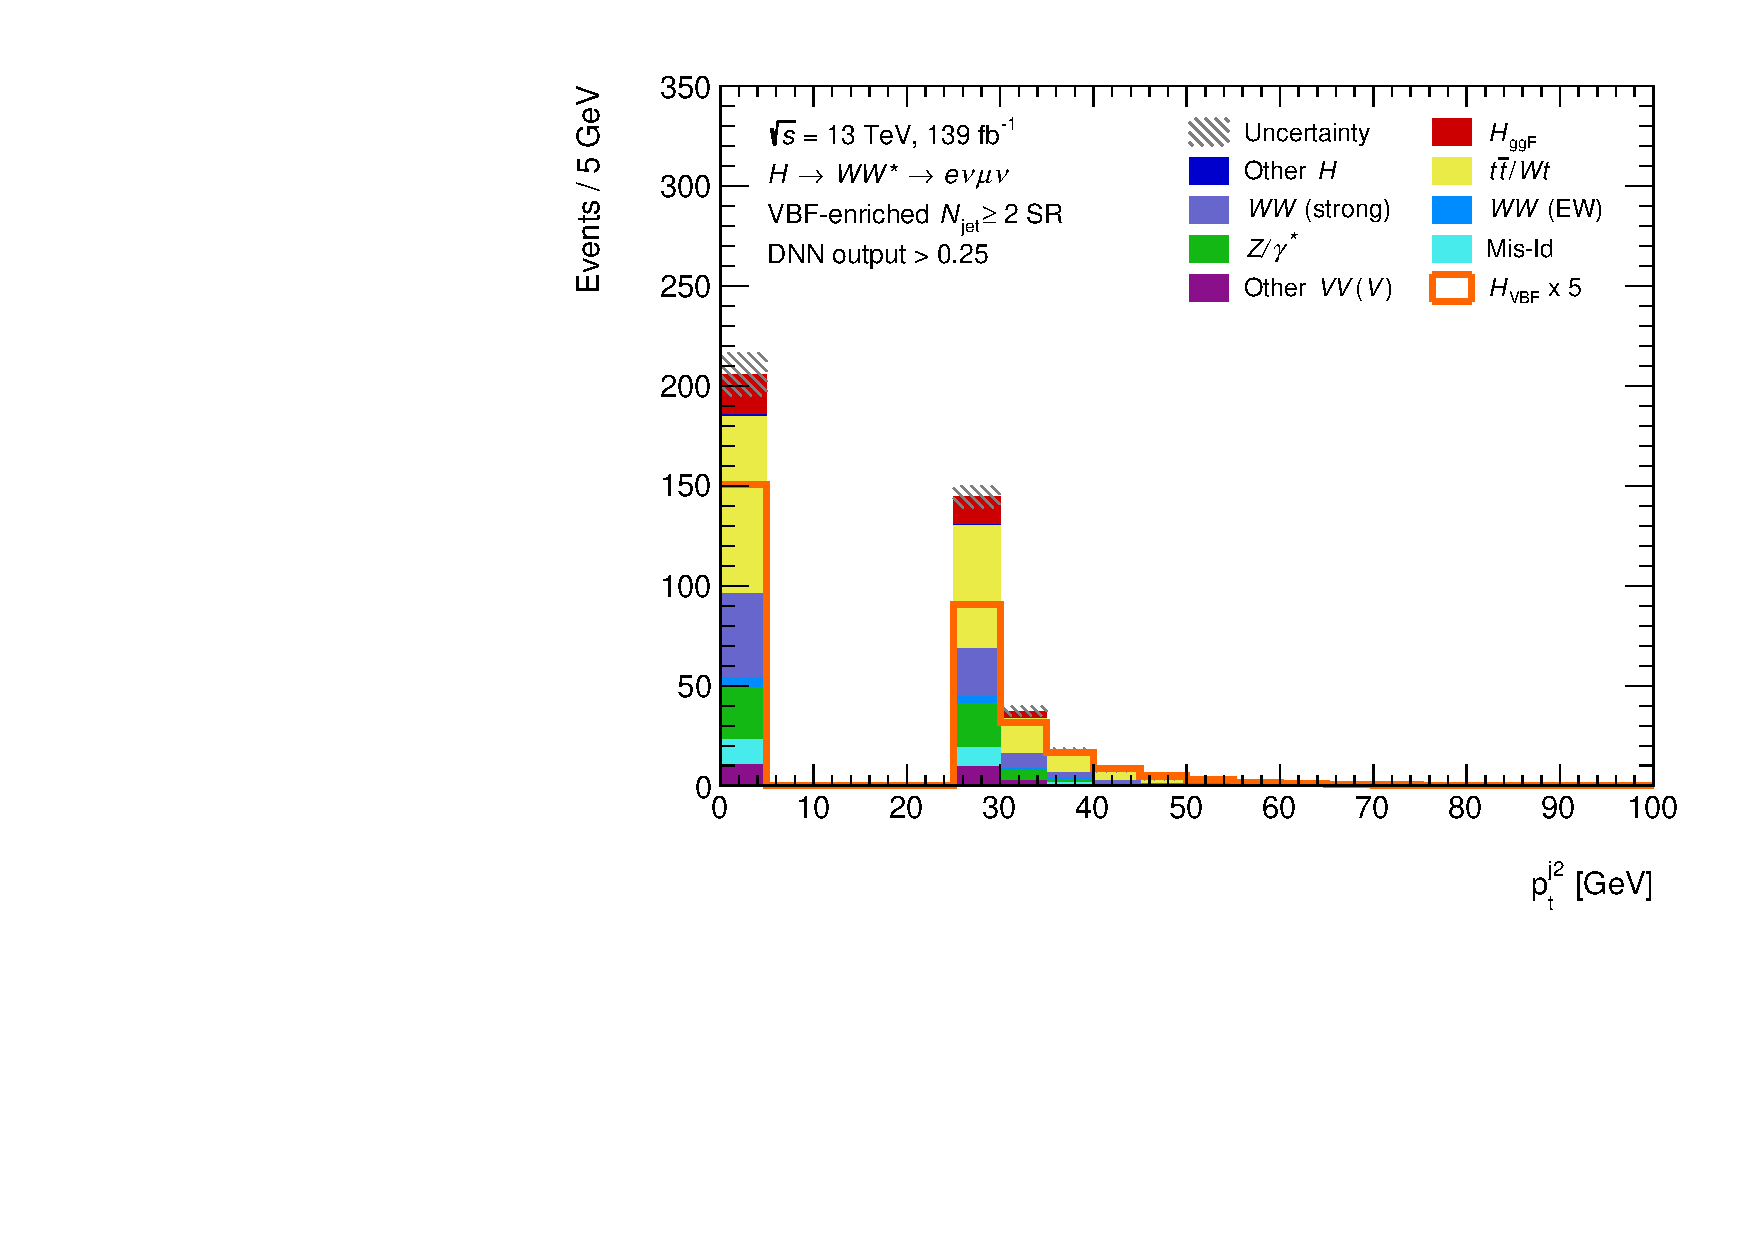
\includegraphics[width=0.32\textwidth]{figures/hww/dnn/blinded/run2-emme-CutVBFSR_DNN25-thirdJetPt-lin.pdf} \hfill
        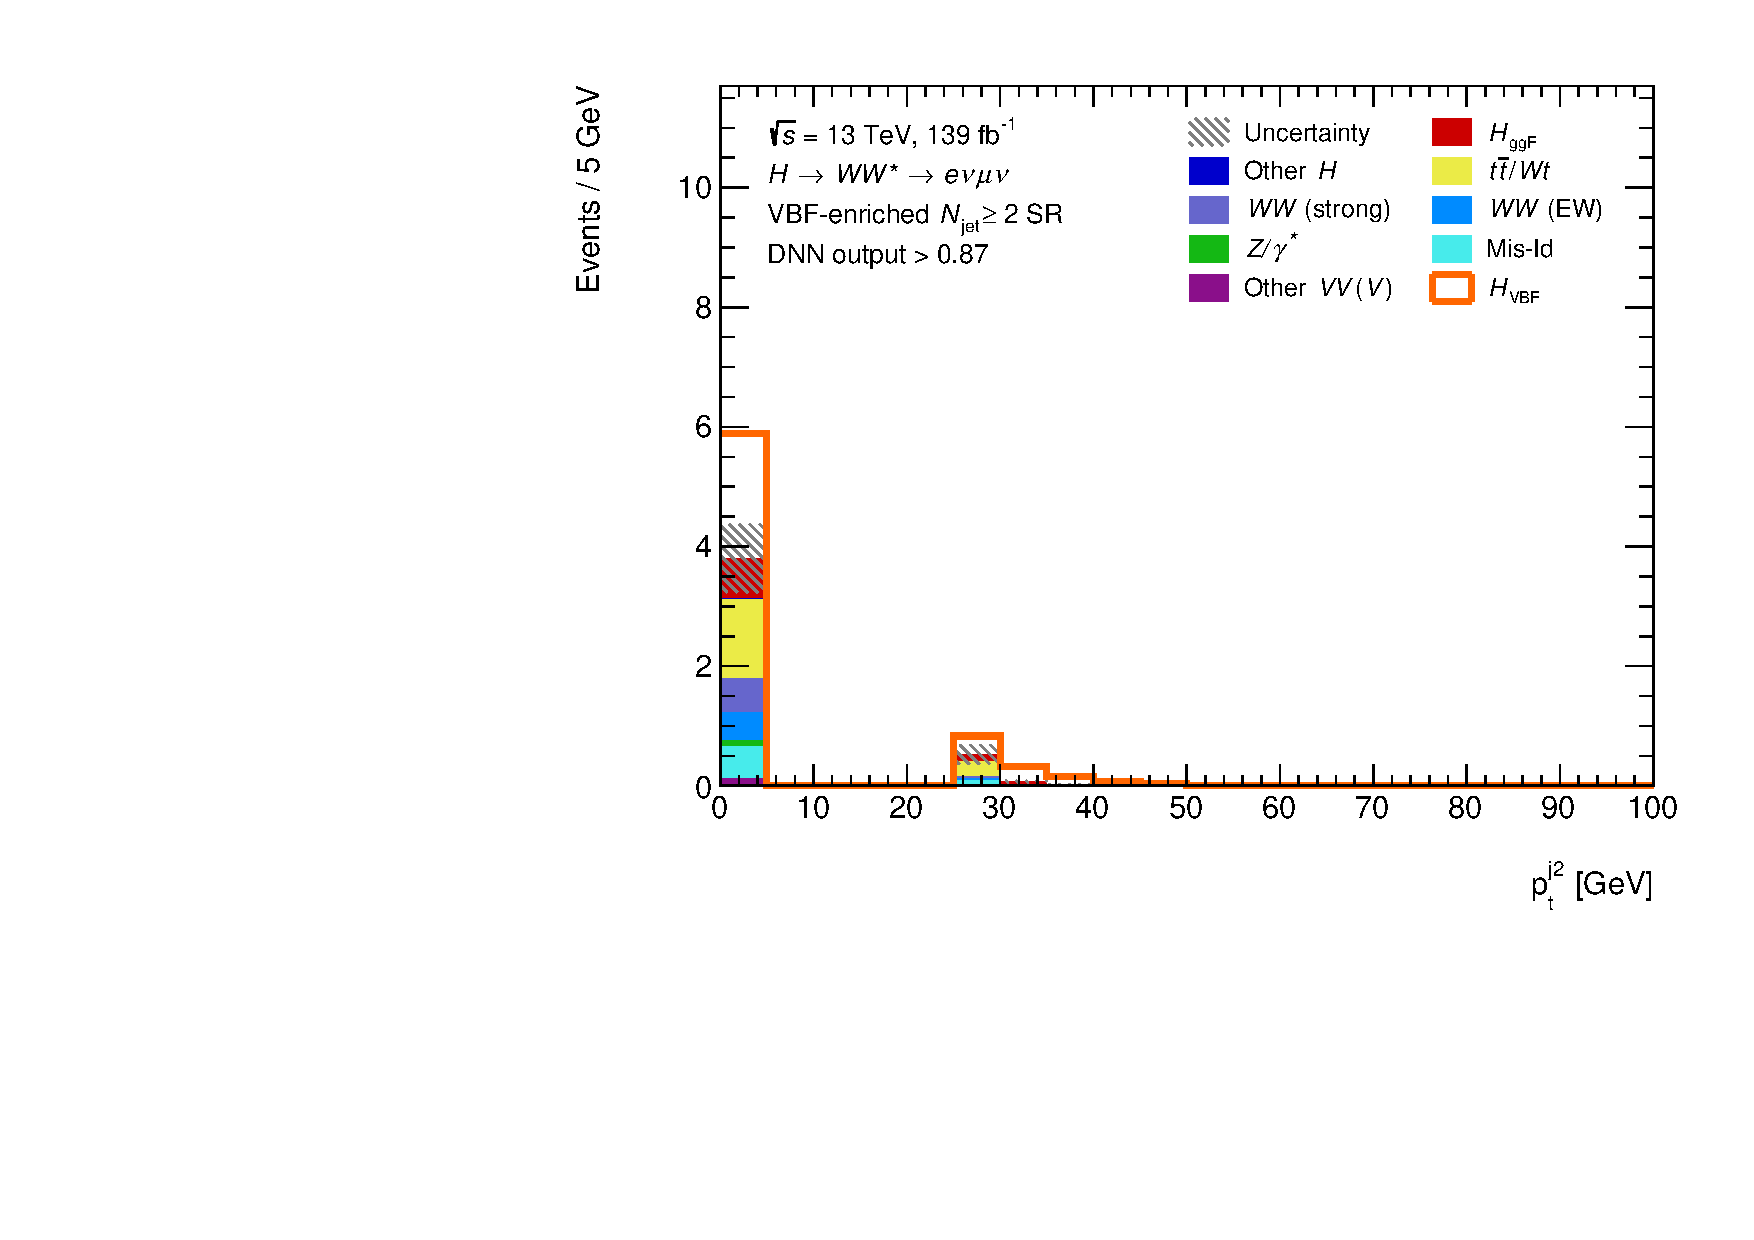
\includegraphics[width=0.32\textwidth]{figures/hww/dnn/blinded/run2-emme-CutVBFSR_DNN87-thirdJetPt-lin.pdf}
    } 
    {\caption{Distributions of $\pTjone$, $\pTjtwo$, and $\pTjthree$ in the VBF signal region.
            Each row shows one variable with different cuts on the DNN output distribution being applied in different columns.
            \label{app:fig:dnn-inputs-vbf-top2} }}
\end{figure}


\begin{figure}[h]
    \centering
    \subfloat[$\dphill$]{
        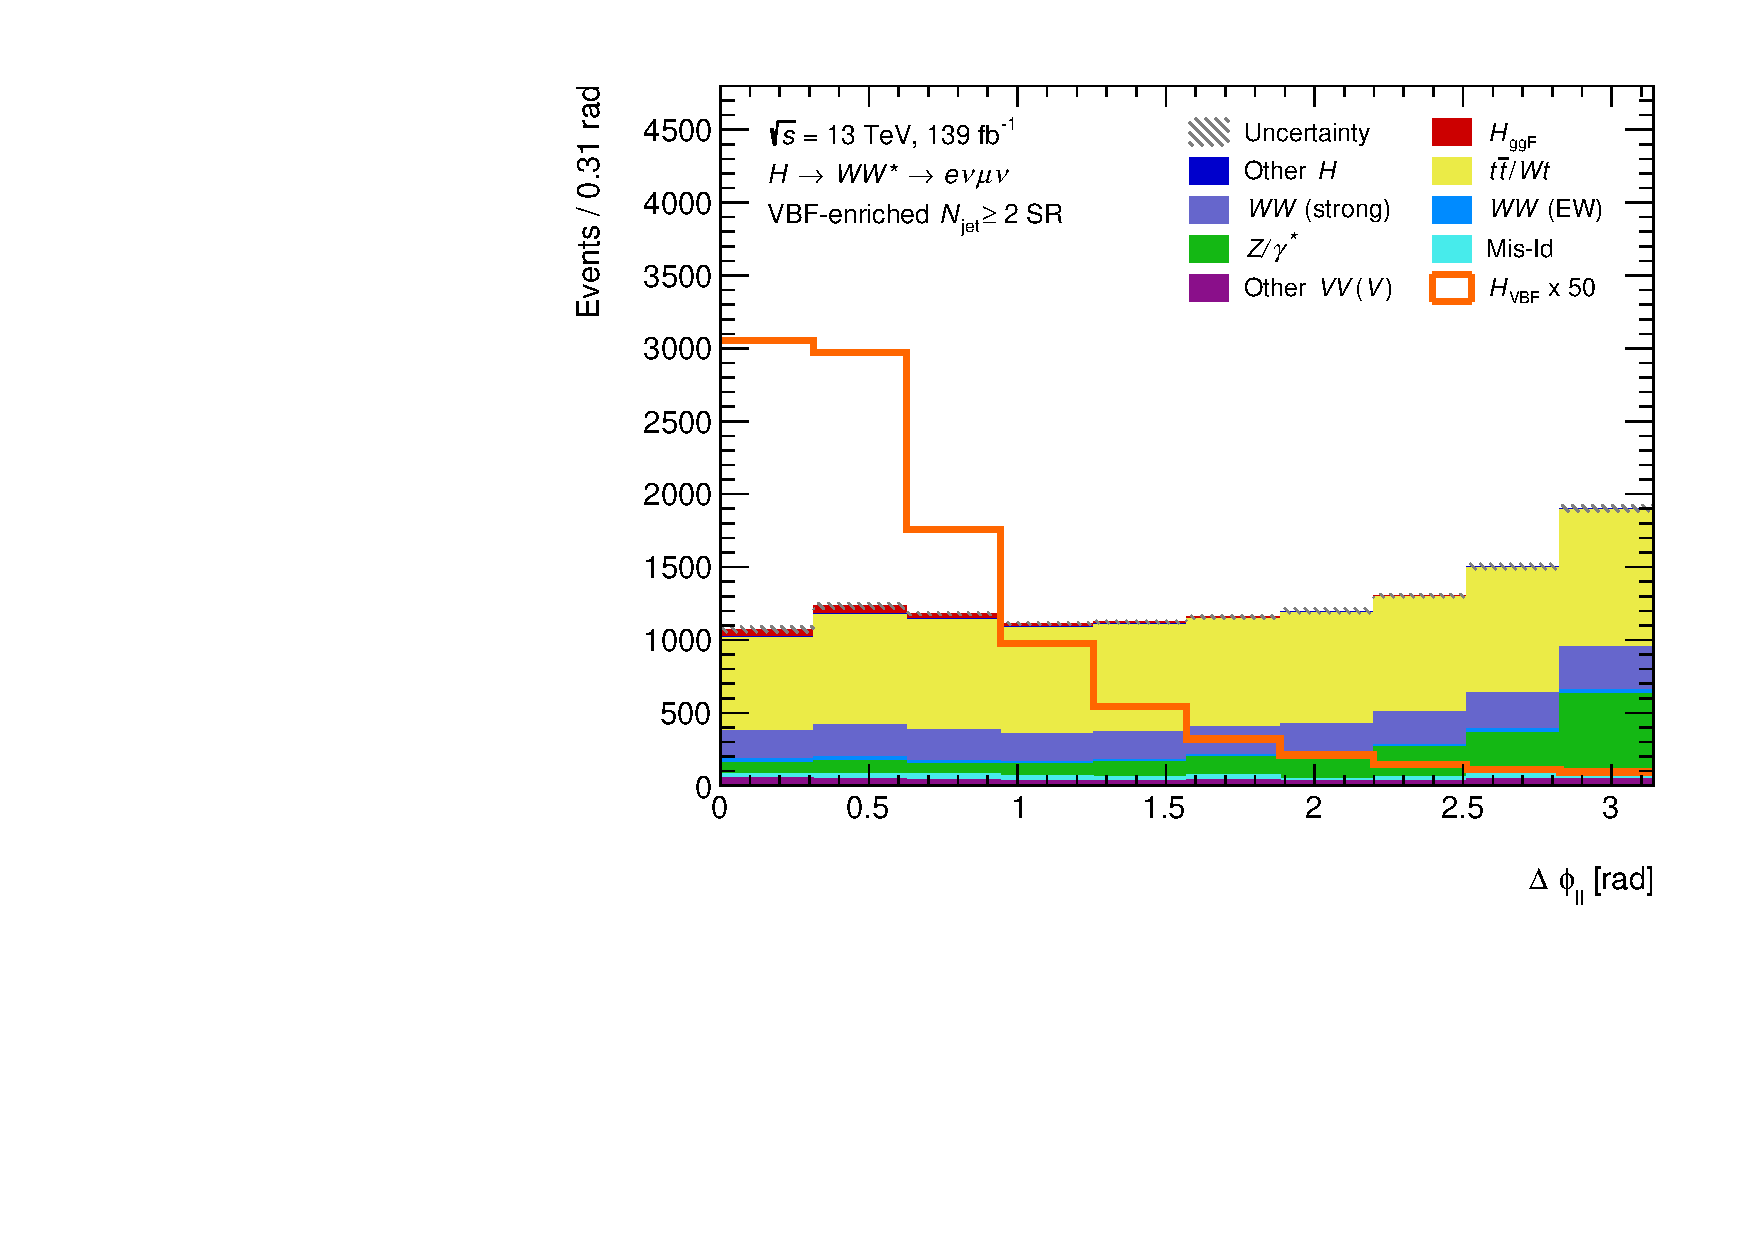
\includegraphics[width=0.32\textwidth]{figures/hww/dnn/blinded/run2-emme-CutVBF_SR-DPhill-lin.pdf} \hfill
        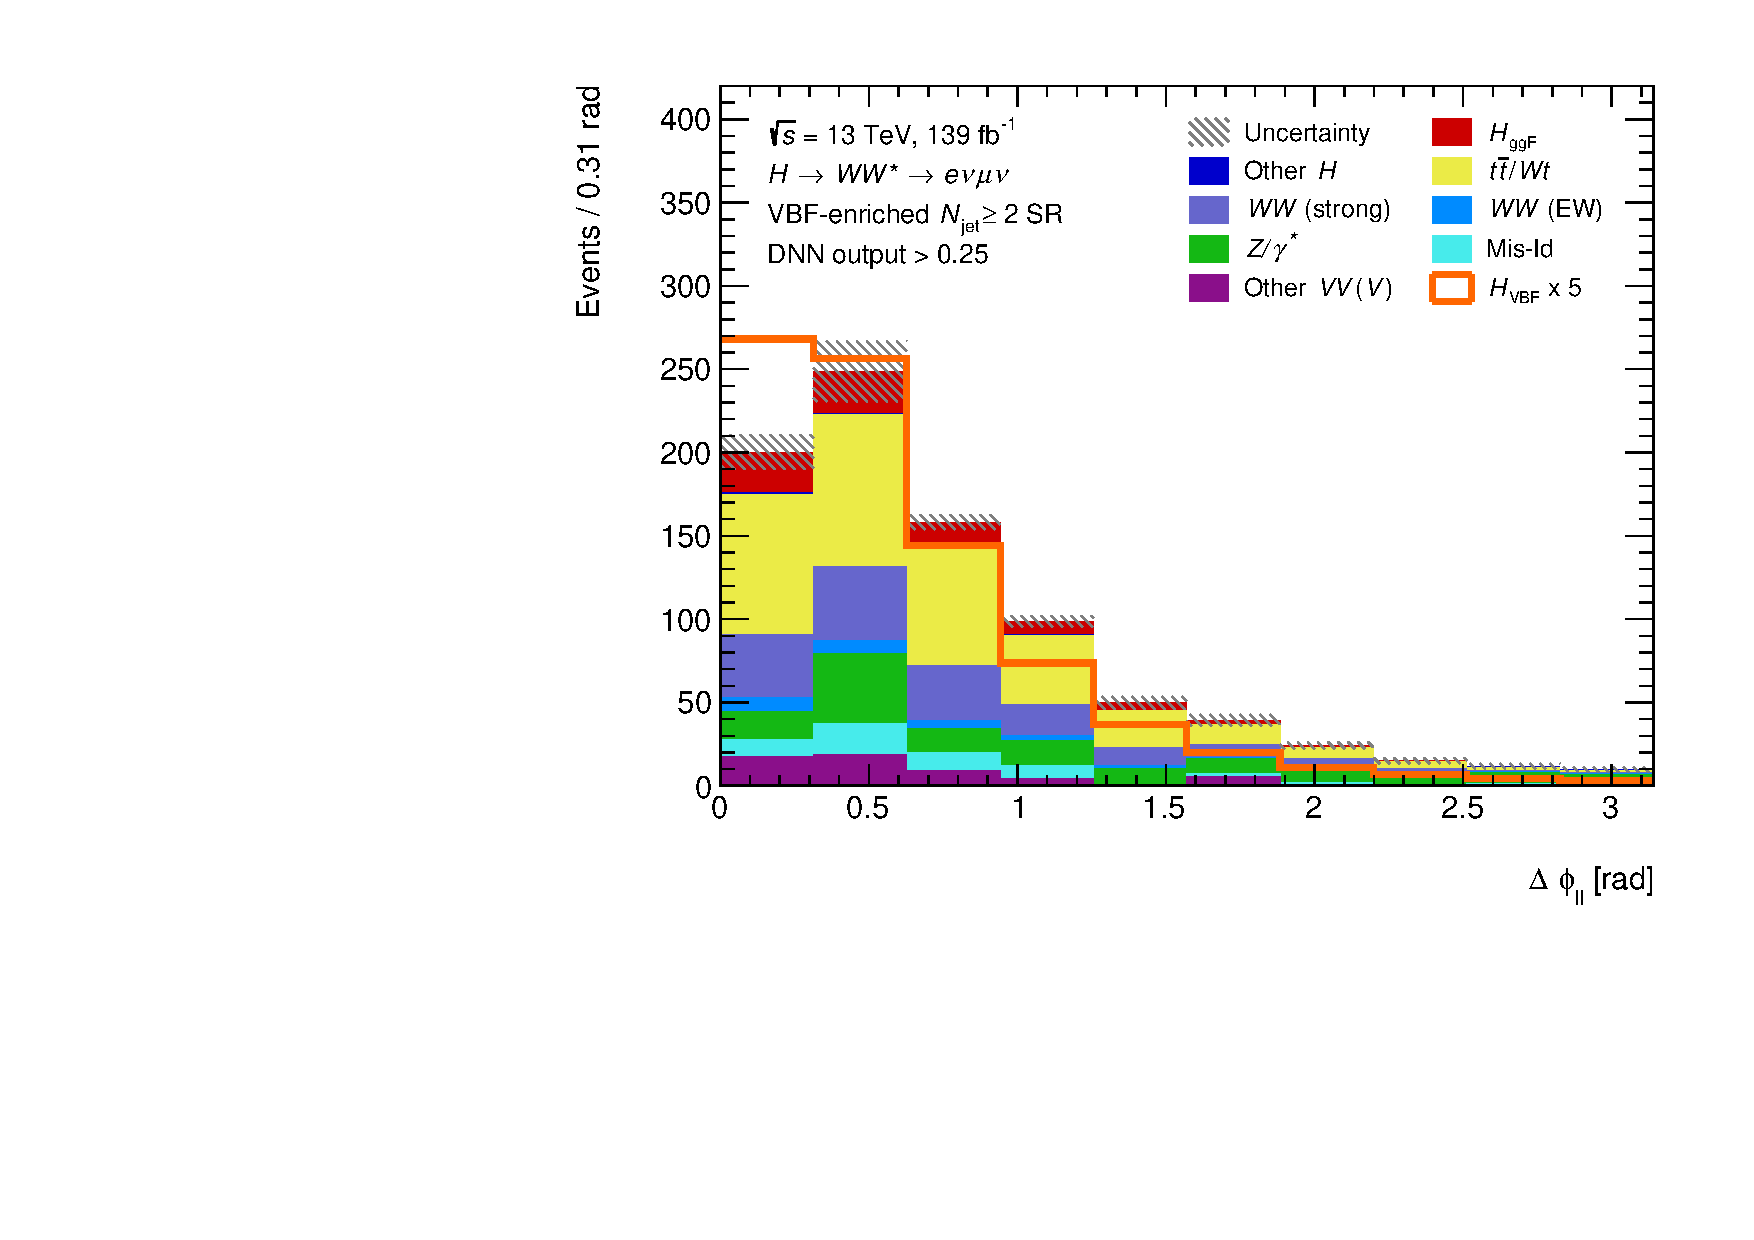
\includegraphics[width=0.32\textwidth]{figures/hww/dnn/blinded/run2-emme-CutVBFSR_DNN25-DPhill-lin.pdf} \hfill
        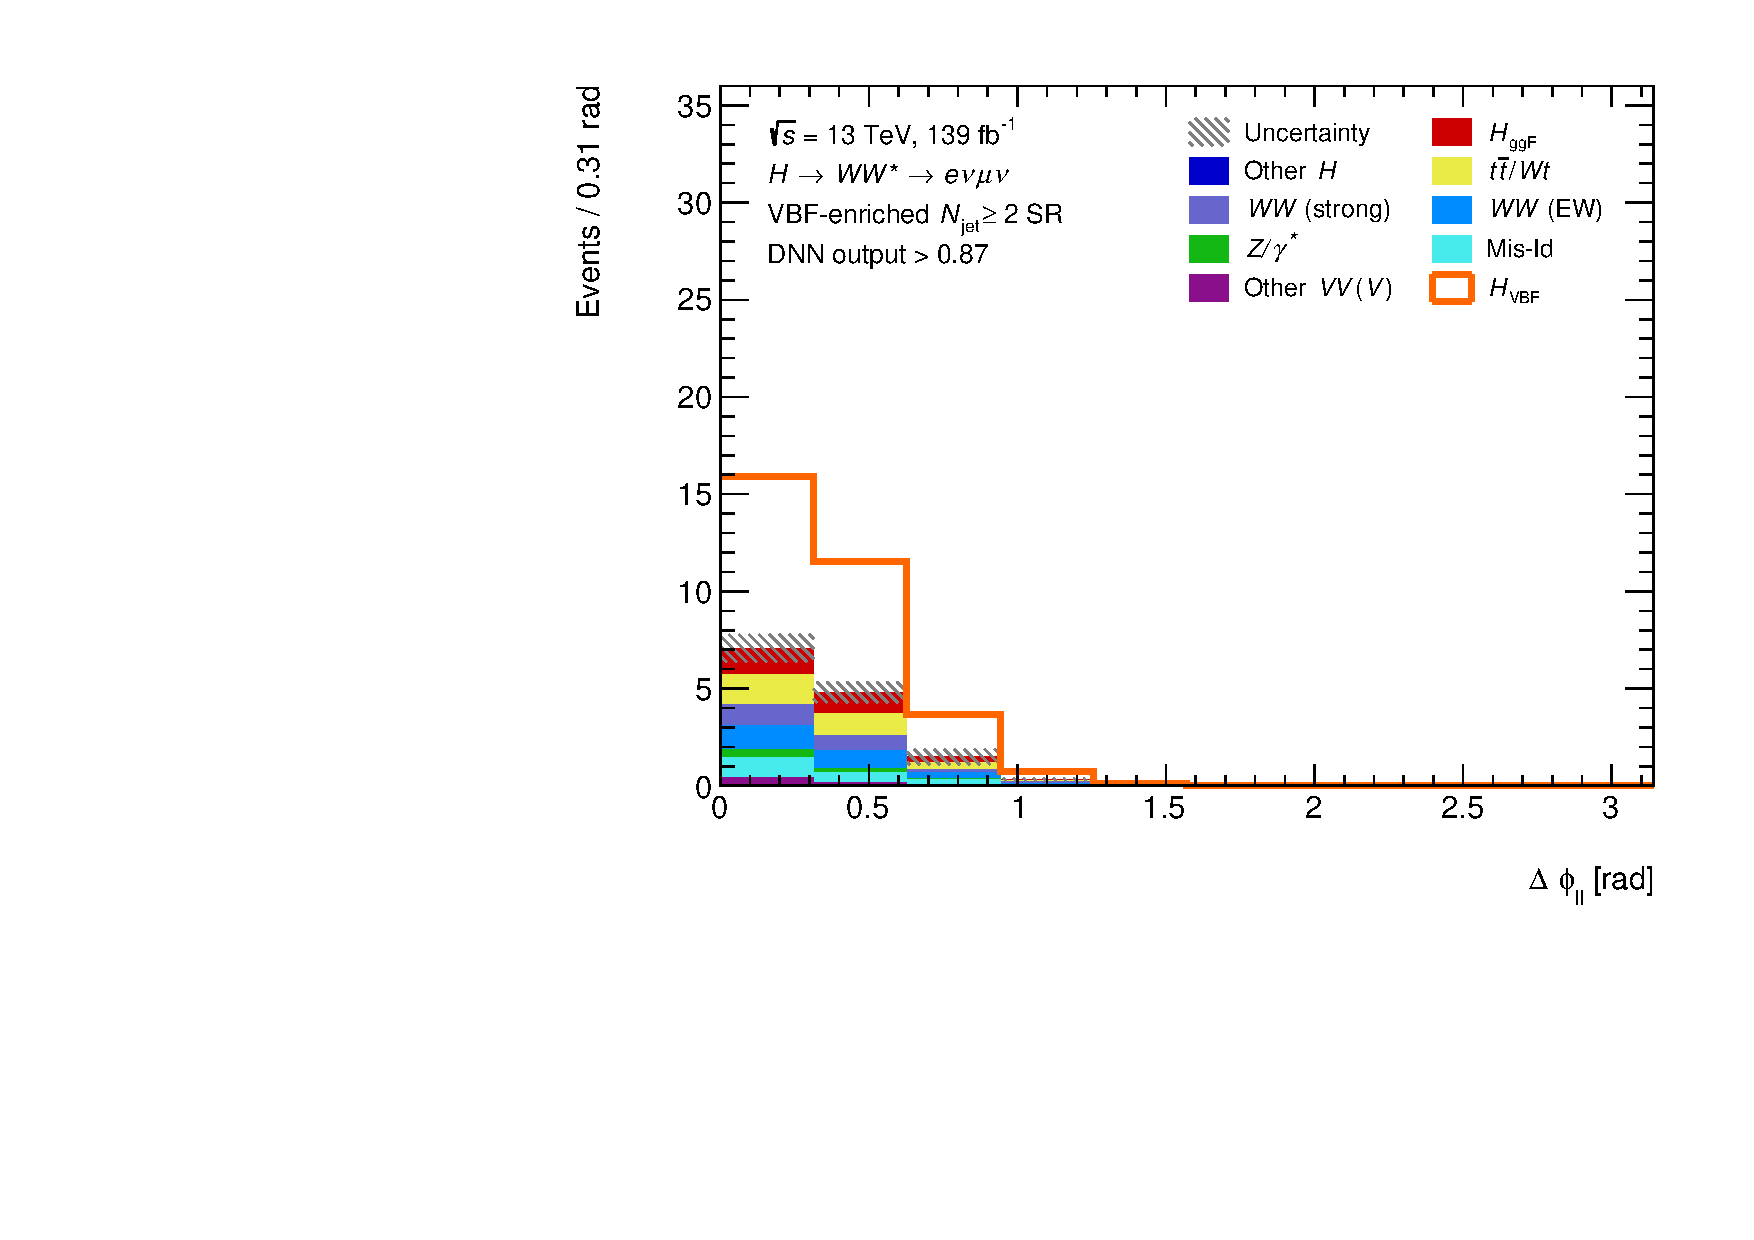
\includegraphics[width=0.32\textwidth]{figures/hww/dnn/blinded/run2-emme-CutVBFSR_DNN87-DPhill-lin.pdf}
    } \\
    \subfloat[$\mll$]{
        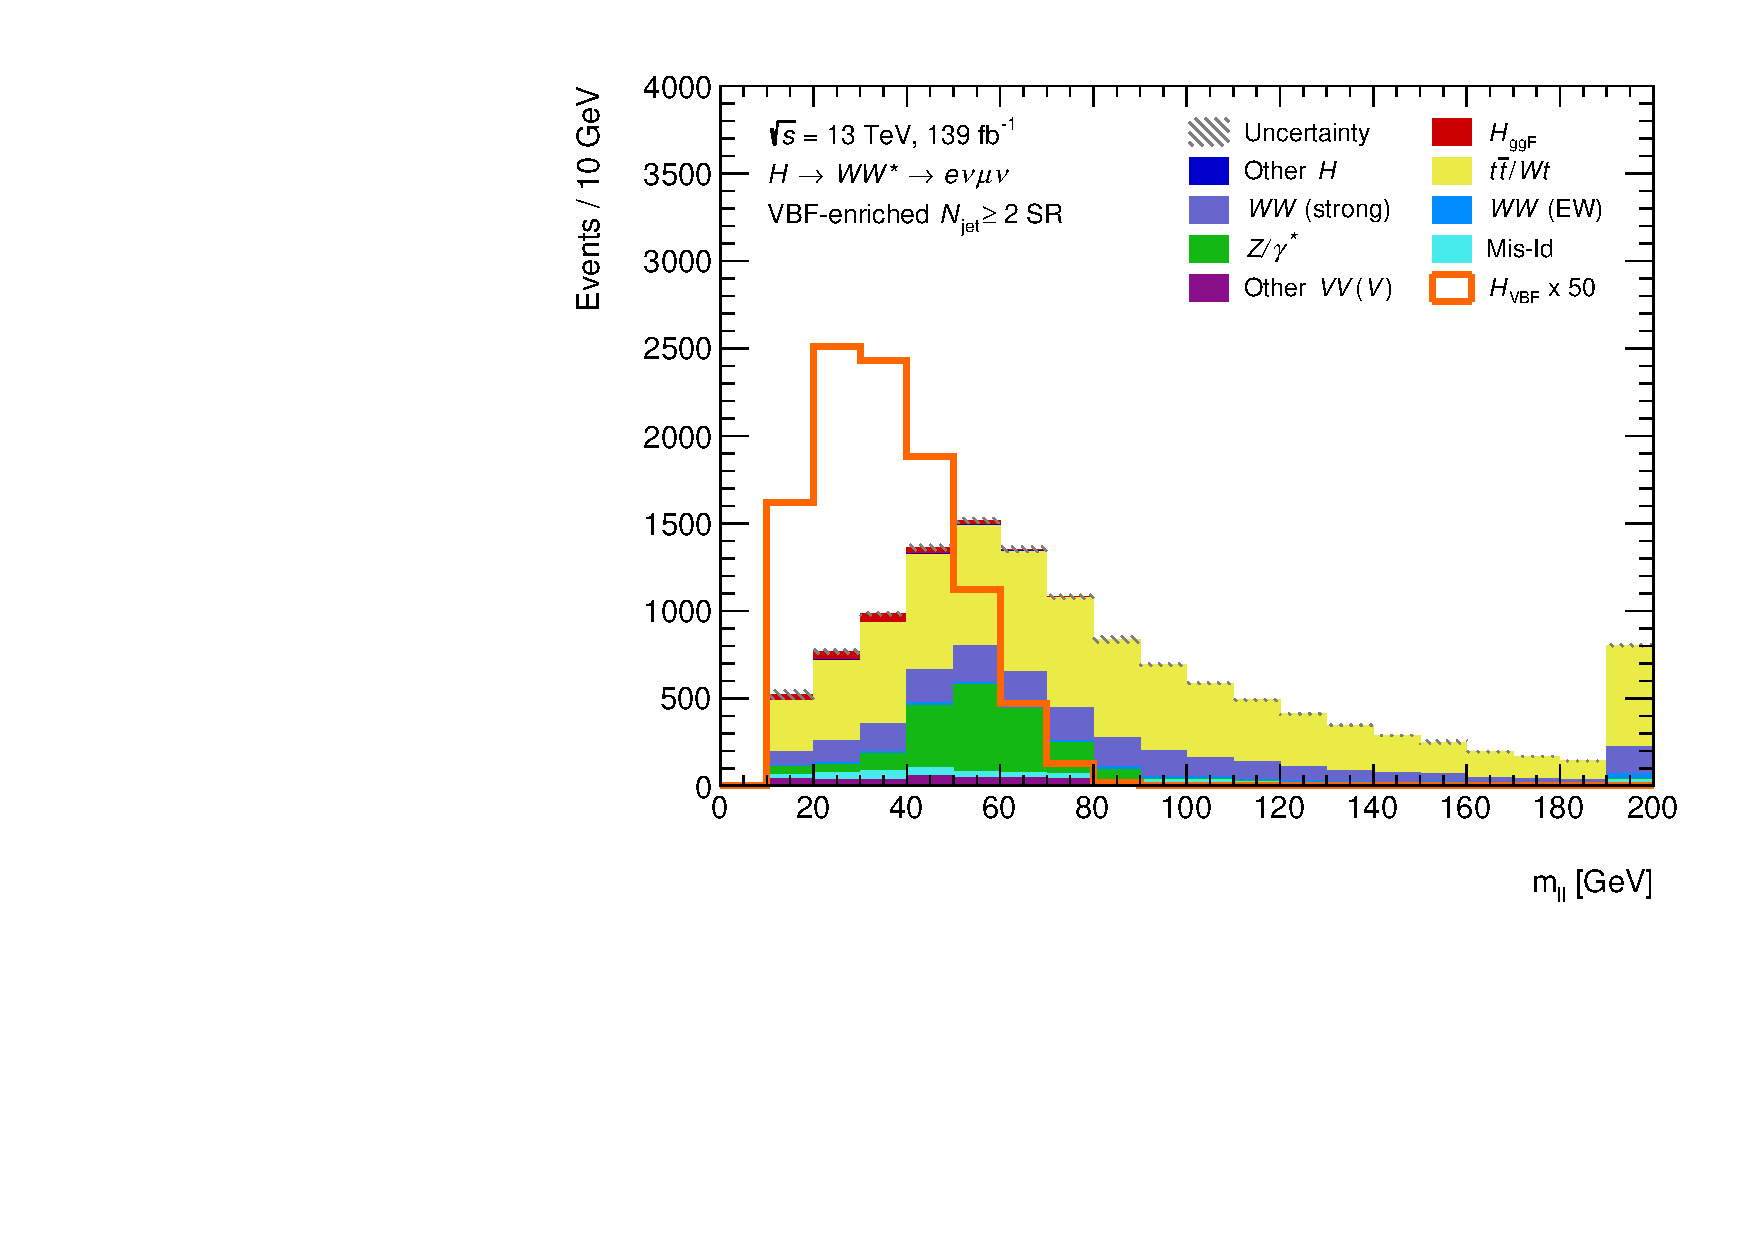
\includegraphics[width=0.32\textwidth]{figures/hww/dnn/blinded/run2-emme-CutVBF_SR-Mll-lin.pdf}
        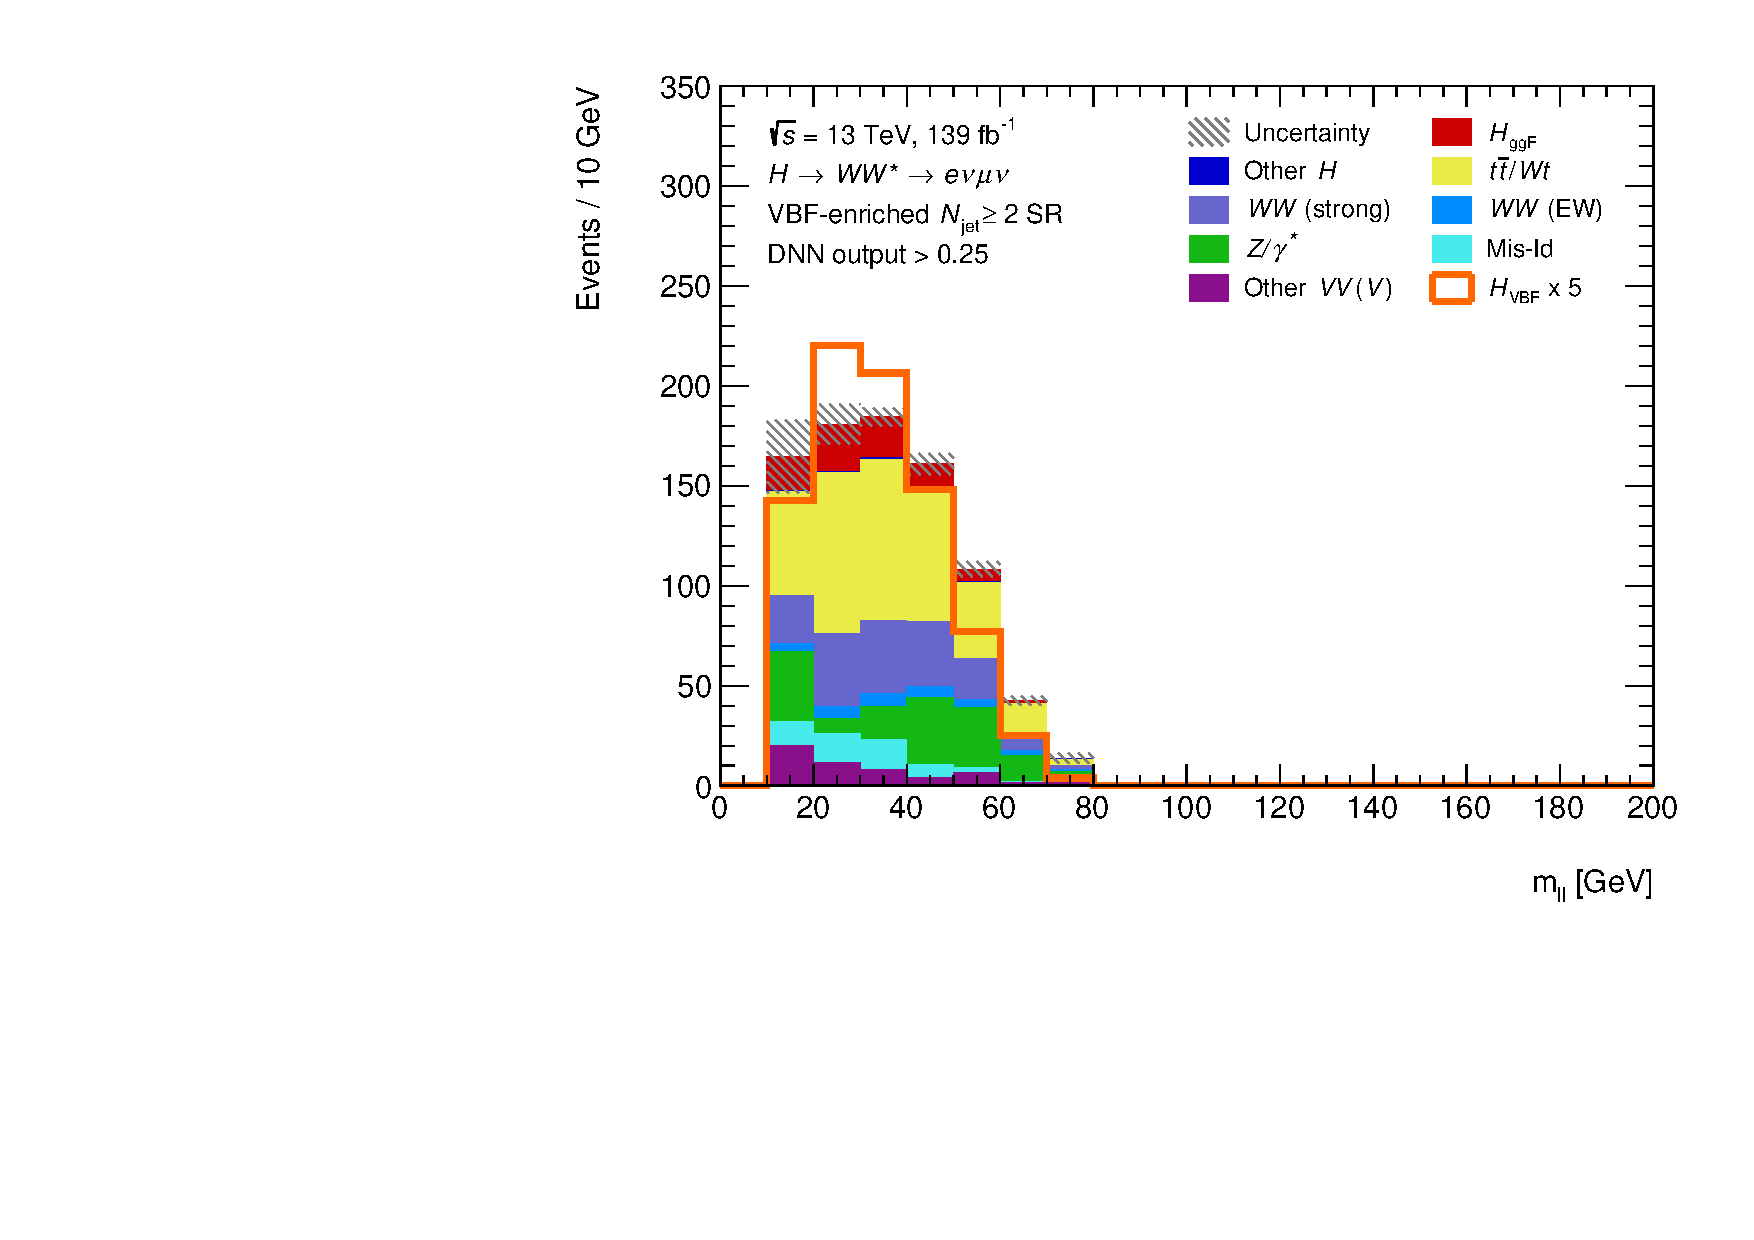
\includegraphics[width=0.32\textwidth]{figures/hww/dnn/blinded/run2-emme-CutVBFSR_DNN25-Mll-lin.pdf}
        \includegraphics[width=0.32\textwidth]{figures/hww/dnn/blinded/run2-emme-CutVBFSR_DNN87-Mll-lin.pdf}
    } \\
    \subfloat[$\mT$]{
        \includegraphics[width=0.32\textwidth]{figures/hww/dnn/blinded/run2-emme-CutVBF_SR-MT-lin.pdf} \hfill
        \includegraphics[width=0.32\textwidth]{figures/hww/dnn/blinded/run2-emme-CutVBFSR_DNN25-MT-lin.pdf} \hfill
        \includegraphics[width=0.32\textwidth]{figures/hww/dnn/blinded/run2-emme-CutVBFSR_DNN87-MT-lin.pdf}
    } 
    {\caption{Distributions of $\dphill$, $\mll$, $\mT$ in the VBF signal region.
        Each row corresponds to one variable with different selections made on the DNN output.
        \label{app:fig:dnn-inputs-hwwdecay} }}
\end{figure}



\begin{figure}[h]
    \centering
    \subfloat[$\pttot$]{
        \includegraphics[width=0.32\textwidth]{figures/hww/dnn/blinded/run2-emme-CutVBF_SR-PtTot-lin.pdf} \hfill
        \includegraphics[width=0.32\textwidth]{figures/hww/dnn/blinded/run2-emme-CutVBFSR_DNN25-PtTot-lin.pdf} \hfill
        \includegraphics[width=0.32\textwidth]{figures/hww/dnn/blinded/run2-emme-CutVBFSR_DNN87-PtTot-lin.pdf}
    } \\
    \subfloat[$\METSig$]{
        \includegraphics[width=0.32\textwidth]{figures/hww/dnn/blinded/run2-emme-CutVBF_SR-METSig_broad-lin.pdf} \hfill
        \includegraphics[width=0.32\textwidth]{figures/hww/dnn/blinded/run2-emme-CutVBFSR_DNN25-METSig_broad-lin.pdf} \hfill
        \includegraphics[width=0.32\textwidth]{figures/hww/dnn/blinded/run2-emme-CutVBFSR_DNN87-METSig_broad-lin.pdf}
    } \\
    {\caption{Distributions of $\pttot$ and $\METSig$ in the VBF signal region.
            Each row shows one variable with different cuts on the DNN output distribution being applied in different columns.
            \label{app:fig:dnn-inputs-top-sup} }}
\end{figure}
}


\subsection{Validation of input features}

\Cref{fig:dnn-features-correlations} shows the correlations between the variables.
\Cref{fig:dnn-features-profiles} shows the profiles of the variables comparing data with the expectation from simulated samples.
\todo{Input Variables Plots}

\begin{figure}[t]
    \subfloat[] {
        \newImageResizeCustom{0.47}{figures/hww/dnn/correlation-matrix-sig.pdf}
    }
    \subfloat[] {
        \newImageResizeCustom{0.47}{figures/hww/dnn/correlation-matrix-bkg.pdf}
    }
    \caption{Correlation matrix of the input features used in the VBF DNN for (a) the VBF signal and (b) the non-VBF-signal processes.}
    \label{fig:dnn-features-correlations}
\end{figure}


\begin{figure}[t]
    \includegraphics[width=\textwidth,trim=45 0 45 0]{figures/hww/dnn/correlations_PROF_SR.pdf}
    \caption{Profiles of all combinations of DNN input features.}
    \label{fig:dnn-features-profiles}
\end{figure}

\subsection{Re-training the DNN and optimizing sample fraction}
\label{subsec:sample-fraction-optimization}
This is case in the VBF analysis, where systematic uncertainties of particular processes dominate the measurement uncertainties, and thus finding ways to train the DNN with putting more emphasis on the suppression of the processes with large uncertainties. 

Final optimization:
-  BKG weights (EWWW scan)!
-  Significances W/ and W/O syst uncertainties, W/ rebinning! (final optimization)

% Significance Z0:
% hww_syst_unc = {"Vgamma": 1, "otherVV":0.12, "Zjets": 0.25, "WW":0.3, "EWWW": 0.5, "singletop":0.5, "ttbar":0.3, "ggF":0.5, "VBF":0.3}


% Plots made with SFUsMLKit on cedar with:
% ./plot.py -c configs/HWW/winningSubmission.cfg --trainingFolderName dropout-02-5-fold-aggressive-lr-schedule-2-fine-scan-ewww-scan-etafix/210805_9_0.12_8226149877761426764
\begin{figure}[t]
    \subfloat[] {
        \newImageResizeCustom{0.47}{figures/plots/sample-fractions/sig_vs_lrate.pdf}
    }
    \subfloat[] {
        \newImageResizeCustom{0.47}{figures/plots/sample-fractions/sig_vs_ew_fraction_lr9.pdf}
    }
    \caption{}
    \label{fig:ew-fraction-scan}
\end{figure}

\subsection{Final model validation}

The distributions in \cref{fig:dnn-train-vs-test} show that the model generalizes very well.

- Plots with data (also LINEAR ONE! that was not approved by ATLAS? is that allowed?!)
\todo{Add plots of variables in different DNN bins!}


\begin{figure}[t]
    \subfloat[] {
        \newImageResizeCustom{0.49}{figures/hww/dnn/train_vs_test_dnn_score_normalized_log.pdf}
    }
    \subfloat[] {
        \newImageResizeCustom{0.49}{figures/hww/dnn/train_vs_test_dnn_score_zoom_non-normalized_non-log.pdf}
    }
    \caption{Comparison of the DNN output distributions of the training set and test set corresponding to the training data for (a) the full range of DNN output values and (b) the region with high VBF signal purity.}
    \label{fig:dnn-train-vs-test}
\end{figure}
